\documentclass{wustlthesis}
\setmainfont{Times New Roman}               % Use Times New Roman


% Re-calculate the lengths of a text line using the current font
\setlxvchars[\normalfont\normalsize]
\setxlvchars[\normalfont\normalsize]
\checkandfixthelayout[classic]

% Enable refinements of typographics
\usepackage[
    activate=true,
    disable=false,  % enable microtype even in the draft mode
    babel=true,     % enable language-specific kerning.
]{microtype}
\DeclareMicrotypeAlias{Times New Roman}{ptm}

% Hyperlinks
\usepackage{hyperref}
\hypersetup{%
    colorlinks=true,
    linkcolor=black,
    urlcolor=blue,
    citecolor=black,
}
% default URL style
\urlstyle{same}

% Tables (optional packages)
\usepackage{threeparttable}
\usepackage{makecell}  % allow multiple lines in a table cell
\usepackage{multirow}   % allow multiple lines in a table cell

% Graphics
\usepackage{graphicx}

% Subcaptions
% The caption format is "Figure 1. Some caption. (A) subcaption. (B) subcaption".
% And the label reference format is "Figure 1A".
\usepackage{subcaption}
\renewcommand\thesubfigure{\Alph{subfigure}}
\renewcommand\thesubtable{\Alph{subtable}}
\captionsetup{subrefformat=parens}
% Enable subcaption for supplemental figures/tables.
% The caption format is "Supplemental Figure S1. Some caption. (A) …. (B) …."
% and the label reference format is "Figure S1A".
\DeclareCaptionSubType{suppfigure}
\DeclareCaptionSubType{supptable}
\renewcommand\thesubsuppfigure{\Alph{subsuppfigure}}
\renewcommand\thesubsupptable{\Alph{subsupptable}}

% Allowing subcaptions when all figure panels are combined
% into one source image. Based on https://tex.stackexchange.com/a/255790
\newcommand{\phantomlabel}[1]{%
    \parbox{0pt}{\phantomsubcaption\label{#1}}%
}

% Add a note for figure caption spanning multiple pages
\newcommand{\legendcontdnote}{%
    \sourceatright[2em]{%
        \footnotesize\itshape(legend continued on next page)%
}}
\newcommand{\legendcontdref}[1]{%
    \emph{(\fref{#1} continued)}%
}



% Bibliography
% use BibLaTeX + Biber and Nature citation style.
% some extra configurations:
%   - Hide ISBN and URL
%   - Display DOI
%   - Show up to 9 authors
%   - Enable back references
\usepackage[backend=bibtex,authordate, giveninits=false,
uniquename=mininit, natbib]{biblatex-chicago}
\def\citeapos#1{\citeauthor{#1}'s (\citeyear{#1})}



% Change colors of urls
\usepackage{xcolor}
\definecolor{navy}{HTML}{2F729C}
\definecolor{darkred}{rgb}{0.55, 0.0, 0.0}
\usepackage{hyperref}
\hypersetup{colorlinks, citecolor=navy, linkcolor=black, urlcolor=navy}

\usepackage{float}
\usepackage{caption}

\renewcommand{\bibname}{Reference}
\usepackage{setspace}
\usepackage{multicol}
\usepackage{tikz}
\usetikzlibrary{shapes,arrows,positioning,matrix}
\tikzstyle{arrow} = [thick,->,>=stealth]
\usepackage{pifont}
\usepackage{listings}
\lstset{
  basicstyle=\ttfamily\small,
  backgroundcolor=\color{white},
  frame=single,
  breaklines=true,
  captionpos=b,
  numbers=left,
  numberstyle=\tiny\color{white},
  xleftmargin=0pt,
  xrightmargin=0pt,
  keywordstyle=\color{black},
  stringstyle=\color{purple},
  commentstyle=\color{green},
  showstringspaces=false,
  tabsize=4
}


% define the bibliography path
\addbibresource{MyLibrary}



% Configure title page
\settitle{A Big Voice in a Small Democracy: Three Papers on American Local Politics}
\setauthor{Lucas Boschelli}
\setthesistype{Dissertation}
\setthesisdegree{Doctor of Philosophy}
\setthesisdegreeabbrv{Ph.D.}
% Degree officially earn date must be in December, May, or August
\setdegreedatemy{May}{2024}
\setthesiscommittee{%
    Betsy Sinclair, Chair\\
    Dino Christenson \\
    Andrew Reeves\\
    Christopher Lucas\\
    Janet Box-Steffensmeier}
\setthesisschool{School of Arts \& Sciences}
\setthesisdepartment{Department of Political Science}
\setthesispresentee{Washington University in St.\@ Louis}
\setthesisabstractfulldegree{%
    \thesisdegree\ in Political Science\\
    \thesisdepartment}
\setthesisadvisorwithtitle{%
    Professor Betsy Sinclair, Chair\\}


% Configure PDF metadata
\hypersetup{
    pdftitle={%
    A Big Voice in a Small Democracy: Three Papers on American Local Politics
    },
    pdfauthor={\thesisauthor},
}


% Optional packages that are not required in the real thesis
\usepackage[shortlabels]{enumitem}   % Custom list structures (lettered list)
\setlist{noitemsep}
\usepackage{layout}     % Show page layout
\usepackage{pifont}     % Extra symbols (optional if the main font has the symbols)
\usepackage{emoji}      % Emojis

% Optional styling that is not required in the real thesis
\newcommand*{\file}[1]{\texttt{#1}}


\begin{document}

\thetitlepage                       % Title page
\frontmatter
\thesiscopyright{%                  % Thesis copyright page
    \textcopyright~\degreeearnyear, Lucas Boschelli}

\SingleSpacing*
\setSingleSpace{1.15}
\tableofcontents*                   % Table of contents (ToC)
\listoffigures                      % List of figures (LoF)
\listoftables                       % List of tables (LoT)

\DoubleSpacing
\setPagenoteSpacing{1}  % single spacing for footnotes
\thesisacknowledgments

An acknowledgments page must be included in your final dissertation or thesis.  If you wish to
include a special dedication you can either use it to close the acknowledgments page or place it on
the page that immediately follows.  The acknowledgments page should be listed in the table of
contents.  Place it after the final list used in the document, and before any dedication, abstract,
or epigraph that is included.

It is appropriate to acknowledge sources of academic and financial support; some fellowships and
grants require acknowledgment.

We offer special thanks to the Washington University School of Engineering for allowing us to use
their dissertation and thesis template as a starting point for the development of this document.

\null\hfill \thesisauthor

\noindent
\textit{Washington University in St.\@ Louis}\\
\textit{May 2017}
    % Acknowledgements
\thesisdedication{%                 % Dedication page
    Dedicated to everyone who helped me thrive.}

\begin{abstract}
An individual's greatest political voice is often within America's smallest democracies. Through three papers, this dissertation explores three key dimensions of political participation within America's local governments: representation, evaluation, and coverage. The first paper explores the question of whether a more accessible local government is a more representative one. By leveraging the switch to online meetings induced by the COVID-19 pandemic, I analyze whether the shift to more accessible meetings promotes healthy democratic participation or amplifies pre-existing inequities in local political participation. To accomplish this, I first construct a novel dataset of public meeting minutes from 2018 until 2022 for county, municipal, and school board governments within the St. Louis region. I then combine public participation data from these minutes with existing political and demographic datasets. Through a time-series cross-sectional analysis, I find that virtual meetings significantly increased participation in some local contexts but did not affect or decreased participation in others. Importantly, I find evidence that while virtual meetings experience similar inequalities in who participates as in offline meetings, they garner greater participation from women in county and school board governments.\\ 

Before individuals decide whether to voice their concerns to a local government, they must, in some way, evaluate its performance. In the second paper, I examine how individuals form these evaluations and whether and how an individual's partisan identity may shape their evaluations. I argue that for some services, for which parties hold ideologically distanced and distinctly homogeneous opinions, evaluations of local services will be biased toward their party's average position regardless of a service's actual performance. To test this theory, I examine individual's evaluations of their local schools and police. Through a cross-sectional analysis of national survey respondents matched to measures of their local conditions, I find that for polarized services such as policing, individuals have a systematic bias in favor of their party's position regardless of the service's objective performance. Additionally, this bias exists irrespective of the partisan control of state and local governments.\\

Finally, in the third paper, I introduce a promising framework to address a problem often hindering our coverage of local political data: the transformation of text-based sources. Political and legal texts include many meaningful data we need as researchers to quantify; however, these texts are often too complex to transform automatically and require slow and costly hand coding to do so correctly. I propose a novel approach: a human-in-the-loop pipeline that leverages Large Language Models (LLMs) to crowdsource and transform text-based sources into quantifiable datasets. Through case studies in local and judicial politics, I demonstrate that LLMs are a cost-effective alternative, producing results comparable to professional coders while significantly reducing transformation time. By easing the costs to process text-based sources, this framework promises to improve the accessibility of research and the coverage of important political outcomes.\\

Overall, this dissertation makes significant contributions to understanding political participation in America's local governments by examining representation, evaluation, and coverage. It not only sheds light on the complexities and inequities of local democratic participation within an increasingly nationalized context but also introduces innovative methods to expand our understanding of local political dynamics.
\end{abstract}

\mainmatter
\pagestyle{main}
\chapter{Is a More Accessible Local Government a More Representative One? The Effects of Online Public Meetings}
\label{chap:dissertation-parts}
    
    
    In response to the growing COVID-19 pandemic, the Denver City Council began hosting their general public meetings online, allowing citizens to attend and participate in discussions virtually. This switch was largely positive for the council, seemingly increasing attendance and active engagement with its meetings. In light of these benefits, and at the request of the public, the council decided to maintain online access to their meetings even after switching back to in-person meetings. Denver was not alone in this continuation of pandemic-era online meetings. Numerous other local governments across the country, citing improved access, still allow citizens to participate or at least watch public meetings virtually.\footnote{Some notable examples include municipal and county governments in Chicago, IL, St. Louis, MO, and Austin, TX} Despite this evidence of success, there has been relatively little work examining the empirical effects these online meetings have on political participation within local governments.

    Public meetings, in particular, are a critical component of American local democracy. They allow citizens to participate directly in the policy-making process \citep{adamsPublicMeetingsDemocratic2004} and act as a conduit through which local officials can learn constituent preferences \citep{einsteinMayorsPartisanshipRedistribution2018,choExperimentingPublicEngagement2021,fungVarietiesParticipationComplex2006}. However, participation in these meetings is rare, and those who attend tend to be socially or economically advantaged compared to their surrounding communities \citep{einsteinWhoParticipatesLocal2019,yoderDoesPropertyOwnership2020}. Scholars and policy advocates have theorized that by reducing participatory costs, online meetings could address these inequities and increase the number and diversity of meeting participants \citep{icmaReflectingVirtualPublic2020}. Yet, in one of the few studies of online meetings \citet{einsteinStillMutedLimited2022} finds that, in the case of planning and zoning meetings, online access fails to engage under-represented groups, and participants are similarly misrepresentative of their surrounding communities. In light of this work, however, we still know relatively little regarding the long-term impacts online meetings had on American local democracy, especially outside the context of the pandemic. Moreover, it remains to be seen how such structural changes to local meetings may have impacted other forms of local governments, such as county councils or school boards.

    Through this article, I examine online meetings' long-term effect on political participation within local public meetings. By leveraging the staggard switch toward and away from online meetings in the years after the pandemic, I estimate the impact online meetings had on the amount and diversity of meeting participants within county, city, and school board governments. Overall, I find that online meetings had mixed effects on local democracy. They increased the average number of public commenters in the aggregate but did not do so universally across types of local government. Some local governments experienced drastic increases in participation following their switch to online meetings, while others experienced no change. While commenters vary significantly between forms of local governments, online commenters were equally misrepresentative of their surrounding community as their offline counterparts. In the rare instance when online meetings alleviated disparities in who participates, other dimensions of inequities, such as race, were exacerbated. Overall, my results suggest that online meetings are potentially an effective tool to expand access to local governments, but in isolation, they are insufficient to address pre-existing inequities in who participates within local democracy.

    \section{Accessibility and Political Participation}
    Attending a local political meeting is a potentially burdensome form of political participation for many individuals. Meetings are often held late into the evening on weekdays in schools or government centers. Individuals likely have to arrange for things such as transportation or childcare to attend. By allowing individuals to participate virtually, online meetings alleviate many of these associated costs, as individuals can watch and participate from anywhere with internet access. Improving political participation by minimizing its social, monetary, or time-related costs is far from a new concept in the study of political science. A broad literature exists documenting the benefits of improved accessibility on political behavior and representation. In the context of elections, vote-by-mail and same-day registration, initiatives can increase turnout, especially among low-propensity voters \citep{barberParticipatoryPartisanImpacts2020,bonicaAllmailVotingColorado2021}. Online access, in particular, can substantially lower the costs of participation as individuals do not have to be physically present to participate. In some instances, digital participation can increase the turnout of traditionally underrepresented groups and attract groups previously disengaged in politics \citep{kruegerAssessingPotentialInternet2002,daltonParticipationGapSocial2017}. Thus, it is reasonable to expect online meetings to have similar long-term effects as they minimize many of the costs associated with commenting at local public meetings. However, evidence exists that increased accessibility does not necessarily translate into positive political outcomes.

    While improvements in political accessibility may make participating easier, they may not foster diverse participation. Without efforts to mobilize under-represented groups in particular, disparities in participation may be reinforced or amplified \citep{verbaVoiceEqualityCivic1995}. Notable examples of this occurring are early voting reforms \citep{burdenElectionLawsMobilization2014}, online political activism \citep{chanPoliticalInequalityDigital2021}, and 311 services \citep{wichowskyCallResponseNeighborhood2022}. In each instance, the reforms designed to make participation more accessible largely reinforced pre-existing socioeconomic divides. Notably, \citet{einsteinStillMutedLimited2022} conclude in their analysis of the early implementation of online meetings that this lack of engagement was one of the critical reasons online meetings failed to diversify public meetings. Thus, online meetings —even in the long term—may be inadequate to improve the diversity of commenters within local meetings unless accompanied by sufficient mobilization and outreach efforts.

    \section{Meeting Participation Across Local Contexts:}

    As required under most state laws, local governments hold meetings open to the public, and most offer an opportunity for citizens to participate directly in the policy-making process. Despite this, previous studies of participation in public meetings have primarily focused on the context of city governments \citep[e.g.,][]{einsteinWhoParticipatesLocal2019}. And they have done this for a good reason. Cities play a prominent role in individuals' lives and are the local government they are most likely to interact with directly. They also tend to offer a plethora of opportunities for input in local policy-making processes \citep{nabatchiDirectPublicEngagement2014a,pinBridgingGapElectoral2022,choExperimentingPublicEngagement2021,wichowskyCallResponseNeighborhood2022} and often rely on these public meetings to gauge public opinion and learn of issues for their constituents \citep{einsteinMayorsPartisanshipRedistribution2018}. In terms of records, cities are also likely to keep high-quality meeting minutes transcripts, which are vital to constructing public meeting participation datasets. However, cities are just some of the local governments to hold public meetings to learn their citizens' preferences and concerns. Both school boards and county governments offer similar opportunities.

    School boards often use public meetings as a vehicle to guide school closures and curriculum changes. Much akin to municipal governments, school boards host various public meetings and forums to inform constituents of upcoming changes or gather community feedback. These meetings and the community connection they provide can be vital for the success of school boards \citep{morelHowCommunityEngagement2021,stoneCivicCapacityUrban2001,tracySpeakingOutPublic2007}, and public policy scholars have paid increased attention to the impact these meetings have both on policy outcomes \citep{morelTakeoverRaceEducation2018,hartneyPoliticsMarketsPandemics2022} and the individuals who participate within them \citep{nuamahCostParticipatingPoor2021,collinsDoesMeetingStyle2021,nuamahCloseHomePlaceBased2021}. While invaluable to our understanding of direct democracy and public education, most studies only examine individual case studies commonly surrounding school closures and rarely examine how the structure/accessibility of the meetings may influence participation \citep[although see][]{collinsDoesMeetingStyle2021}. Understanding whether school boards exhibit the same levels of inequality well-documented at the municipal level is vital, especially as critical issues surrounding race, gender, and public health are increasingly decided at the school board level.\footnote{As an example, see \citet{hartneyPoliticsMarketsPandemics2022}}

    Despite counties' vital role within the American government, they have primarily remained the ``forgotten government" of local politics. We know little about how public participation and opinion shape county-level politics \citep{bentonAssessmentResearchAmerican2005a}. Previous work surrounding counties has primarily examined how the composition and characteristics of public officials have shaped county outcomes \citep[e.g.,][]{mohrStrategicSpendingDoes2019}. Crucially despite the fact that counties are often constrained by both state and municipal governments \citep{petersonCityLimits1981}, they are responsive to constituent preferences and susceptible to traditional political influences \citep{debenedictis-kessnerPoliticsForgottenGovernments2020}. Thus public meeting participation may, as it does at other levels of local government \citep{einsteinWhoParticipatesLocal2019}, play an influential role in county politics. Counties, much like other local governments, hold regular meetings open to the public. Many of these meetings allow the public to comment directly on agenda item issues or other concerns. County governments often use these meetings to gauge the public's support for new budgets, large infrastructure projects, or electoral changes. During the COVID-19 pandemic, these meetings became a vital source of information and expression for citizens surrounded by ever-changing health guidelines and restrictions \citep{lynchPandemicPolitics2022}. We know very little regarding who attends these meetings, the issues they bring up, or the impact of their participation. Do counties experience similar levels of participation found in other local governments, or are they also forgotten in the eyes of their constituents?

    Whether participation in public meetings—or the impacts of improved accessibility—should differ across these local government levels is unclear. In their book examining elections and democracy within local politics, \citet{oliverLocalElectionsPolitics2012} suggest that political participation fundamentally changes as local governments increase in size, scope, and bias.\footnote{As defined by the authors, bias refers to a government's ability to distribute resources among its constituents.} As local governments grow, individuals tend to engage with politics less as their connection to political issues and political efficacy decrease \citep{oliverDemocracySuburbia2001,schlozmanUnheavenlyChorusUnequal2012}. Thus, in the context of public meetings, we should expect differences in participation between school boards, cities, and counties simply due to their differences across these dimensions. In theory, individuals should participate the most in school board meetings, as their ability to enact direct policy change is the greatest and their ties to school board issues the most tangible. Likewise, participation within county governments should be the least due to the wider variety of issues and constituent preferences they must address.

    However, these early conclusions contrast the historically low participation levels across all levels of local government \citep{hopkinsIncreasinglyUnitedStates2018}. Local political issues are often parochial and temporal \citep{oliverLocalElectionsPolitics2012}. The habitual nature and value of repeat participation in national-level politics may not exist in local politics \citep{aldrichTurnoutHabit2011}. While events such as school closings, zoning decisions, or election administration are significant political events for these governments, they likely do not affect individuals on a consistent enough basis to warrant intense engagement \citep[see][]{nuamahCloseHomePlaceBased2021}. Moreover, work such as \citet{hopkinsIncreasinglyUnitedStates2018} or \citet{hershPoliticsPowerHow2020} suggest that individuals care more about national issues and are often disengaged from local political happenings. Therefore, it may not matter how these local governments differ because the American public is equally unengaged across all levels, and participation is dominated by a subset of advantaged individuals \citep[e.g.,][]{einsteinWhoParticipatesLocal2019,yoderDoesPropertyOwnership2020}. Understanding how participation differs between local governments is a critical but unaddressed question in political science. A question this paper hopes to address.

    \section{Public Meeting Data:}
    In order to examine the effects of online meetings and expand coverage beyond previous local boundaries, I construct a novel dataset of public meeting participation from the school board, city, and county governments within St. Louis County, Missouri. I chose St. Louis because of the quality of public records, partly due to Missouri's detailed sunshine law, and the county's many overlapping local governments. By focusing on close or overlapping local governments, I can examine the differential effects online meetings may have while controlling for similar regional, state, or federal factors. All of these are especially important given the surrounding context of the COVID-19 pandemic, which elicited a cooperative response from almost all levels of the American government. In total, I collect records of public participation from 22 school boards, 15 municipal governments, and the county itself. These local governments cover a broad spectrum of sizes, with the largest government being St. Louis County (1,001,982) and the smallest being Brentwood City (8,198). Notably, my sample's city and school board governments are relatively diverse and vary in terms of racial makeup, median income, and home ownership. I provide a more detailed breakdown of my sample's demographics and the selection method used to construct the sample within the Appendix. While far from exhaustive, the novel dataset covers 22\% of the county's municipal populations, 52\% of its school board populations, and the entirety of the county.

    

    For each of these governments, I download and digitize their general meeting minutes from 2018 until late 2022. These are the routine public meetings held by each government. By law, these meetings are open to the public, provide opportunities for public comments, follow a set schedule, and maintain detailed minutes of all topics discussed. Given their routine nature and general purpose, these meetings provide a roughly equivalent comparison point between the three levels of local government within my sample.\footnote{Local governments hold other meetings addressing specific policy issues, such as zoning or industrial development. These meetings are also often open to the public and have been the focus of previous studies of public meeting participation \citep[see][]{einsteinWhoParticipatesLocal2019}.} While each government's meeting minutes vary in terms of how detailed they are, most record the names, addresses, and comments of all individuals who participate in the meeting.\footnote{This includes individuals who submit their comments digitally.} In a few rare instances, local governments only record the total number of commenters present. For these cases, I treat each commenter as a unique individual. I present the detailed breakdown of my final dataset within \autoref{tab:commentSummary}. Overall, my dataset includes over 10,000 unique comments submitted by over 8,000 individuals across approximately 2,213 local political meetings.

    \begin{table}[H] 
        \centering 
        \caption{Summary of Comments Database} 
        \label{tab:commentSummary} 
       \scalebox{1}{
            \begin{tabular}{llcc}
            \\[-1.8ex]\hline 
              \hline \\[-1.8ex] 
            \multicolumn{1}{l}{} & \multicolumn{3}{c}{Level of Government}                              \\ 
            \hline \\[-1.8ex] 
                           & County & City   & School Board     \\
            \hline \\[-1.8ex] 
            Years: & 2018-2022 & 2018-2021 & 2018-2022 \\
            Number of Governments: & 1 & 15 & 22  \\
            Number of Meetings: & $218$ & $1029$ & $966$ \\
            Population Coverage: & $100\%$ & $22\%$ & $52\%$  \\
            First Name: & \ding{51}& \ding{51}& \ding{51}\\
            Last Name:  & \ding{51}& \ding{51}& \ding{51}\\
            Address:  & \ding{51}& \ding{51}& \ding{51}\\
            Number of Comments: & 7069 & 1206 & 1892  \\
            Number of Individuals: & 5621 & 926 & 1555  \\
            Commenting Rate: & 0.56\% & 0.20\% & 0.19\% \\
            \hline\\
            \\[-1.8ex]\hline 
              \hline \\[-1.8ex] 
          \end{tabular}}
          \begin{tablenotes}
              \item {\footnotesize Note:  The table above provides the summary of the universe of comments within the data set. Population coverage refers to the estimated proportion of the population of St. Louis County covered by the sample.}
          \end{tablenotes}
      \end{table}

     
    From this initial dataset, we can gleam some insight into public participation across these levels of government. Participation within these meetings is rare across all three forms of local government.  Only 0.56\% of residents comment at county level meetings over my sample’s four years of coverage, with municipal (0.20\%) and school board (0.19\%) governments experiencing slightly lower rates of participation. Individuals also appear to only comment once within meetings and then disappear from the dataset. In fact across all three levels of local government only 15\% of individuals ever submit more than one comment.\footnote{These low levels of repeat participation are not unique to my dataset. Other datasets of meeting participation such as that from \citet{yoderDoesPropertyOwnership2020} have similarly low levels and cover a far more extensive 10 year timeframe.} On average individuals appear to comment regarding a specific issue and then stop actively participating within local meetings. This pattern falls in line with previous conceptions of local democracy and suggests that participation within this realm is deliberate and motivated \citep{oliverLocalElectionsPolitics2012,nuamahCloseHomePlaceBased2021}. Individuals reach out to their local governments when faced with a pertinent issue and then resume their lives once it has been addressed. In the broader context of this paper, meeting accessibility may be more about encouraging new groups to participate rather than fostering repeat participation. Given the unique overlapping nature of my dataset, I can also examine participation across levels of government.\footnote{To match individuals across levels of local government I fuzzy string match on commenters first and last name. My estimates of cross-level commenting are likely larger than the true rates for my sample.} Are individuals active at one level of local government also active in others? The short answer appears to be no. Cross-level commenting appears exceptionally rare with a little over 1\% of commenters ever commenting at more than one level of local government. While this finding may be a product of the relative short time frame covered by the data, it may provide further evidence of deliberate and conscious participation within local democracy.  Individuals appear to only engage the local government pertaining to their specific issue.\footnote{With in the Appendix I provide further evidence of this through text-analysis. Individuals appear to approach local governments with specific and often jurisdictionally relevant issues.}

    \subsection{Coding Meeting Accessibility:}
    Access to local public meetings took many different forms and styles following the pandemic. Each allowed members of the public to watch and participate to varying degrees in these meetings. I classify each meeting in my sample into three broad categories based on the relative level of accessibility they provide to the general public. First, \emph{Offline} meetings are those with traditional access. Individuals must physically attend these meetings to watch and participate. In most cases, local governments will make audio or video recordings available a few days after the meeting, but individuals must be present to participate. Second, \emph{Livestreamed} meetings are those in which local governments stream the meeting to some internet source, and individuals can watch meetings in real-time. For some governments, individuals can submit comments before the meeting and then watch them be addressed live. Finally, \emph{Virtual} meetings are those in which individuals can attend and participate entirely virtually. These were commonly conducted over videoconferencing software, but some local governments allowed the public to call into the meeting and comment. These categories are agnostic to how local governments conduct their meetings (i.e., whether they use videoconferencing software, email, phone calls, etc.) and focus instead on what they allow citizens to do without being physically present.

    Notably, there are apparent similarities between livestreamed and virtual format meetings. Both improve access to public meetings and allow individuals to attend meetings without being physically present. Individuals do not have to travel to government centers and can theoretically attend from anywhere. Given this similarity, I drop this distinction in some future analyses and codify these meetings as simply \emph{Online}. One critical difference between the two, however, is that virtual meetings offer the chance for deliberation between commenters and local public officials. Active deliberation within public meetings can deepen democratic ties \citep{bryanRealDemocracyNew2010,gastilCivicAwakeningJury2002,fishkinWhenPeopleSpeak2009}, produce more responsive policies \citep{robertsPublicDeliberationAlternative1997,fungVarietiesParticipationComplex2006}, and increase trust in local institutions \citep{carpiniPUBLICDELIBERATIONDISCURSIVE2004}. In fact, experimental evidence finds that simply watching public meetings containing deliberation between officials and the public can increase both individuals' trust in public officials and willingness to attend future meetings \citep{collinsDoesMeetingStyle2021}. An effect that may only increase for individuals who actually participate \citep{gastilCivicAwakeningJury2002,minozziTestingBenefitsPublic2023}. Thus if accessibility matters for public participation in local public meetings, we should see the largest changes in virtual meetings, given their additional capacity for deliberation.

    \begin{figure}[H]
        \centering
         \text{Meeting Accessibility Overtime}\par\medskip
        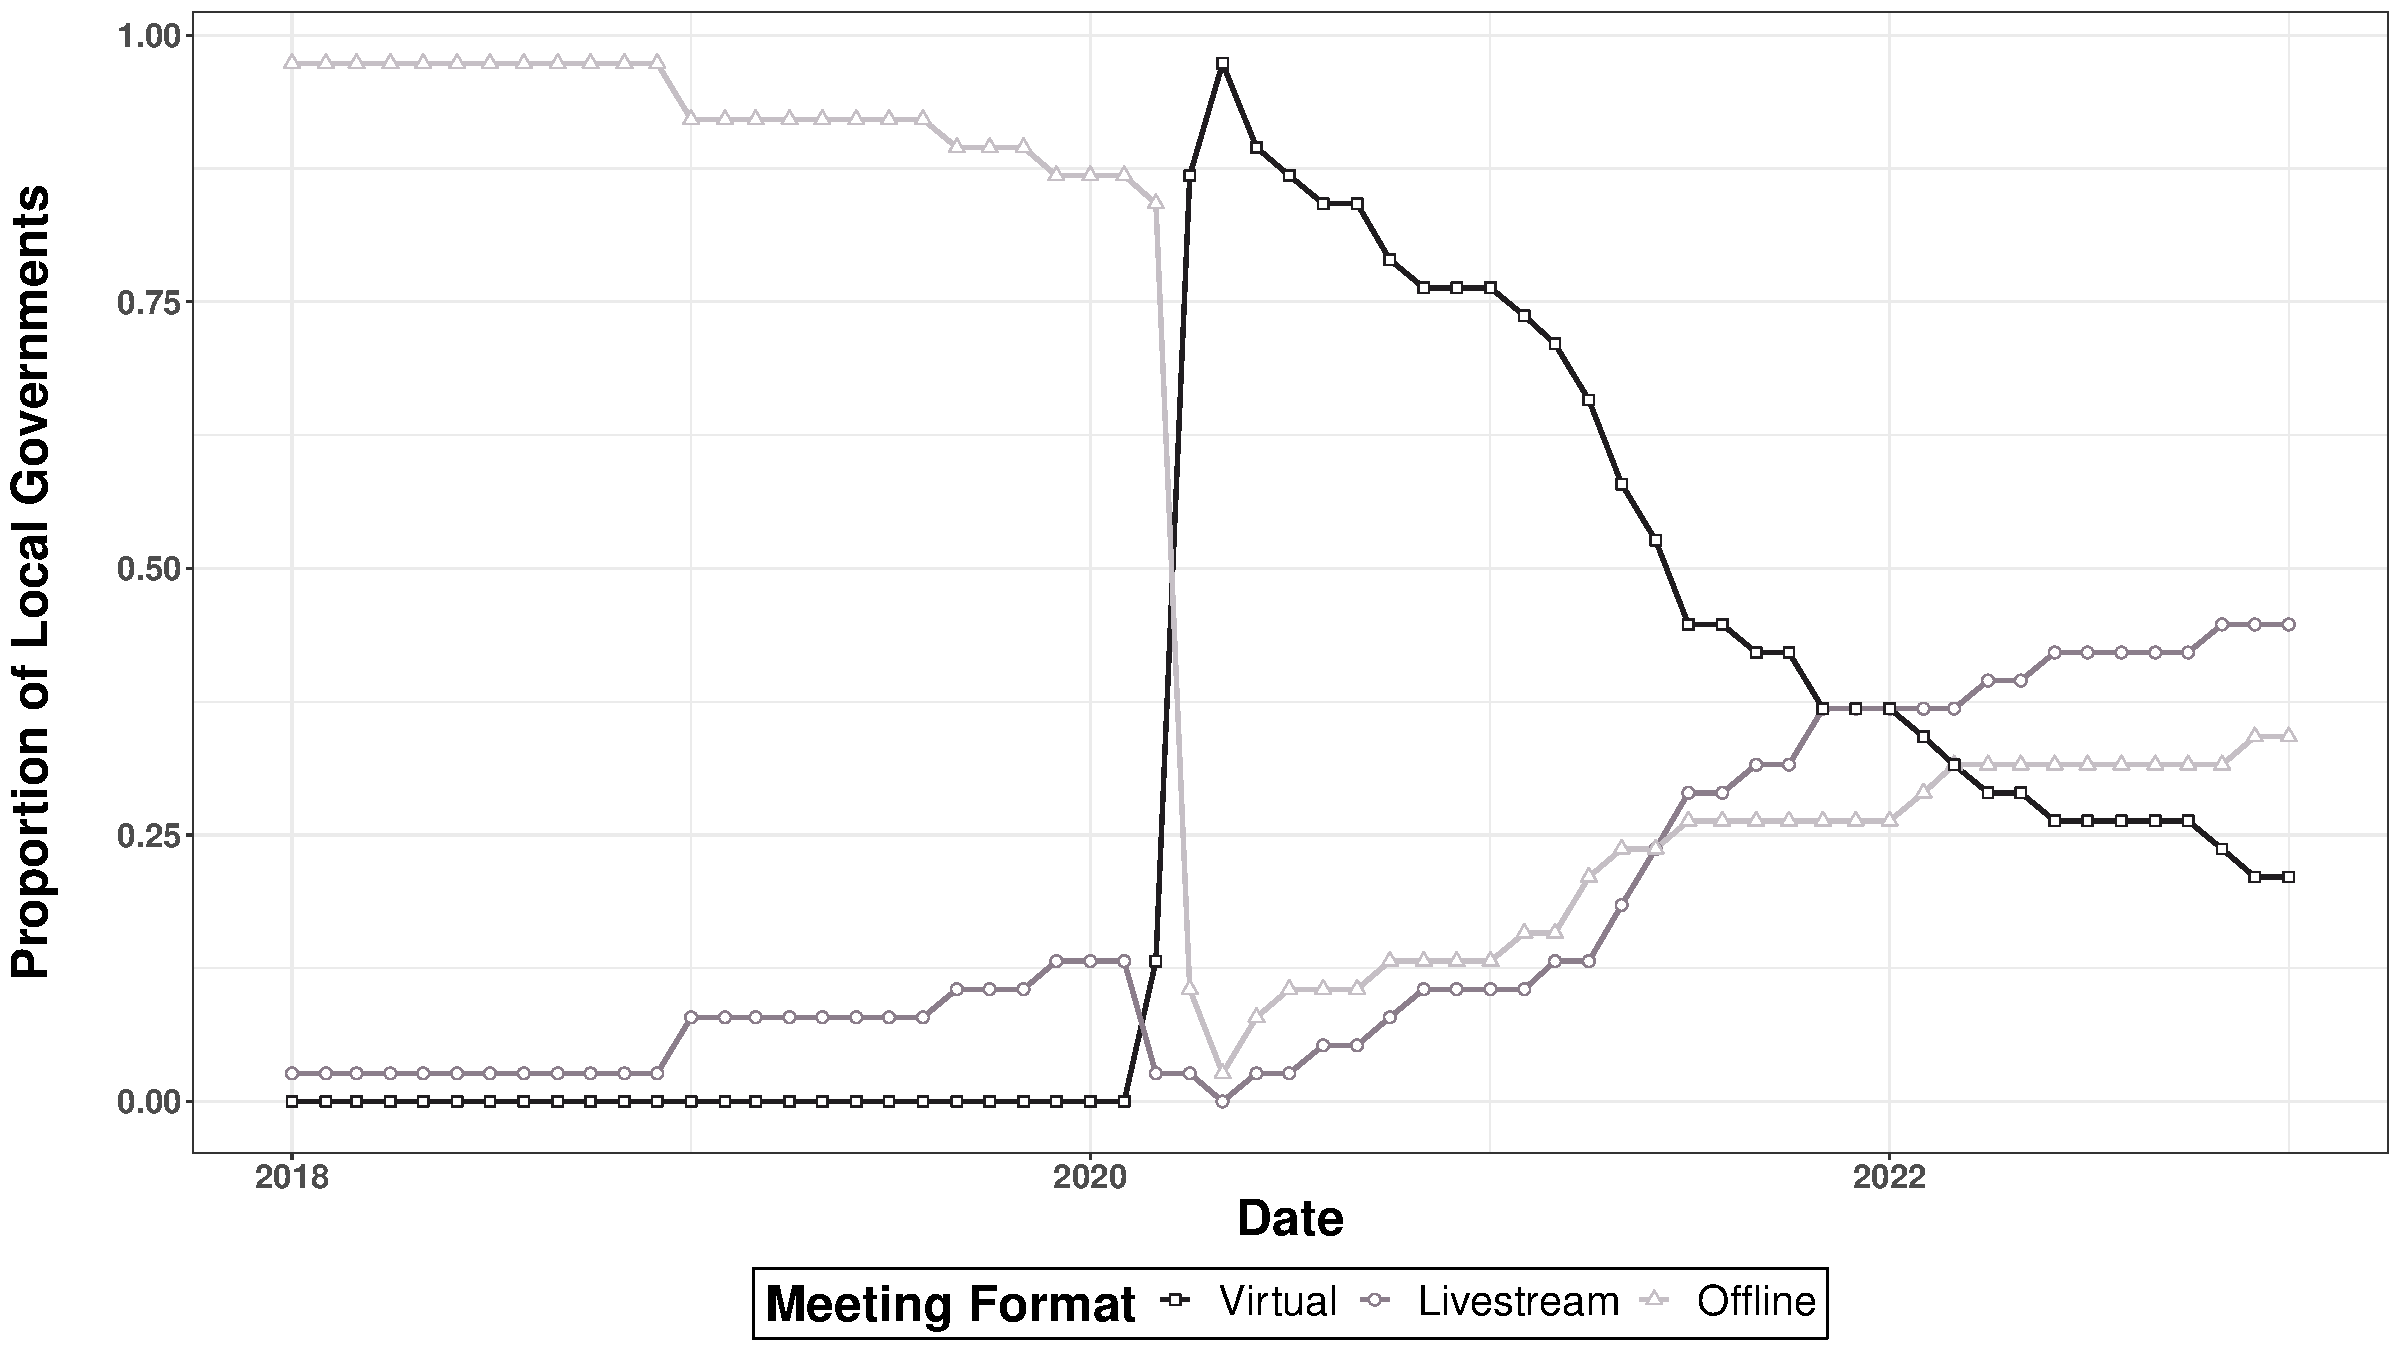
\includegraphics[scale=0.41]{Figures/OverallAccess.pdf}
        \caption[Public Meeting Formats Overtime]{The figure presents the format of local political meetings by month from January 2018 until May 2022.}
        \label{fig:OverallAccess}
    \end{figure}

    For each meeting within my dataset, I classify them into one of the three categories outlined above. As local governments conduct meetings on different schedules and cadences, I aggregate participation and access at the monthly level. I code accessibility based on whether most meetings during a given month belong to one of the three categories. \autoref{fig:OverallAccess} displays access to the local government’s meetings from 2018 until late 2022. I provide similar figures for each level of government within the Appendix. While most governments within my sample held offline meetings before the pandemic, a few cities (18\%) and school boards (6\%) experimented with holding livestreamed meetings beforehand. No governments in my sample held virtual meetings before the pandemic. Following the pandemic, however, every local government appeared to switch to some form of online meeting format. Governments then varied in terms of whether and when they switched away from online meetings, with many choosing to continue hosting online meetings in the years following the pandemic. Interestingly, livestreamed meetings became the modal meeting format for most governments, with offline meetings being the second most common. These trends, however, varied by level of government, with most cities eventually switching back to offline style meetings and both school board and county governments tending to livestreamed meetings. Virtual meetings, while the least common across all three levels of government, were still implemented by a few school board and municipal governments by the end of my sample coverage. In the following section of this paper, I leverage this staggard adoption to (and away from) online meetings to analyze whether the additional accessibility they provide translates to increased and more diverse participation.

    \section{Do Online Meetings Encourage Greater Participation?}
    \subsection{Measuring Effects on Meeting Participation:}

    In response to the developing COVID-19 pandemic, all governments within the state of Missouri were required to hold some form of online meeting from April 2020 until May 2020.\footnote{The exact order was referred to as the ```Stay Home Missouri" Order.} Following the month-long period, local governments could decide whether to switch back to offline meetings or continue hosting their meeting online. This initial shock for local governments provides near perfect opportunity to measure the impact of online meetings on public participation as I can: (1) estimate \emph{within} government effects by comparing governments before and after their switch to online and (2) estimate \emph{between} government effects by comparing governments as they adopt differing meeting formats following the pandemic. The critical question is whether the increased accessibility afforded by online meetings increased rates of public commenting. These meetings should lower the individual costs of participation and hopefully engage additional citizens. To test this initial analysis, I employ the following two-way fixed effects (TWFE) design:

    \begin{equation}\label{mod1}
        Y_{it}=\beta_0+\beta_1D_{it}+\gamma_{i}+\alpha_t+\epsilon_{it}
    \end{equation}

    \noindent where $Y_{it}$ is the total number of participants and $D_{it}$ is an indicator of whether government $i$ held primarily livestreamed, virtual, or online meetings during month $t$. The two-way government ($\gamma_i$) and month ($\alpha_t$) fixed effects to control for the time-invariant characteristics within local governments as well as monthly shocks, which may influence the number of participants at local meetings. Finally, given that I focus on the number of participants within local meetings, I model the above equation using a negative binomial regression.

    To examine whether the effects of online meetings are consistent across levels of local government, I estimate both a pooled and government-level model for each local government in my sample. I utilize the same model definition for both school board and city governments but subset the data to each respective type of government. For inference at the county level, however, my sample only includes a single county government. This fact makes it difficult to employ any form of difference-in-difference design. In order to maintain comparability and interpretability between models, I opt to employ the following simplified model:

    \begin{equation}\label{mod2}
        Y_{t}=\beta_{0}+\beta_1D_{t}+\delta_{t}+\epsilon_{t}
    \end{equation}

    \noindent where I forgo the government and month-fixed effects and substitute $\delta_t$ to capture year-based fixed effects. While this model loses the casual leverage provided by the TWFE modeling approach, it should still provide observational evidence as to whether accessibility matters for county meetings.

    \begin{figure}[H]
        \centering
         \text{The Effect of Meeting Format on Public Meeting Participation}\par\medskip
        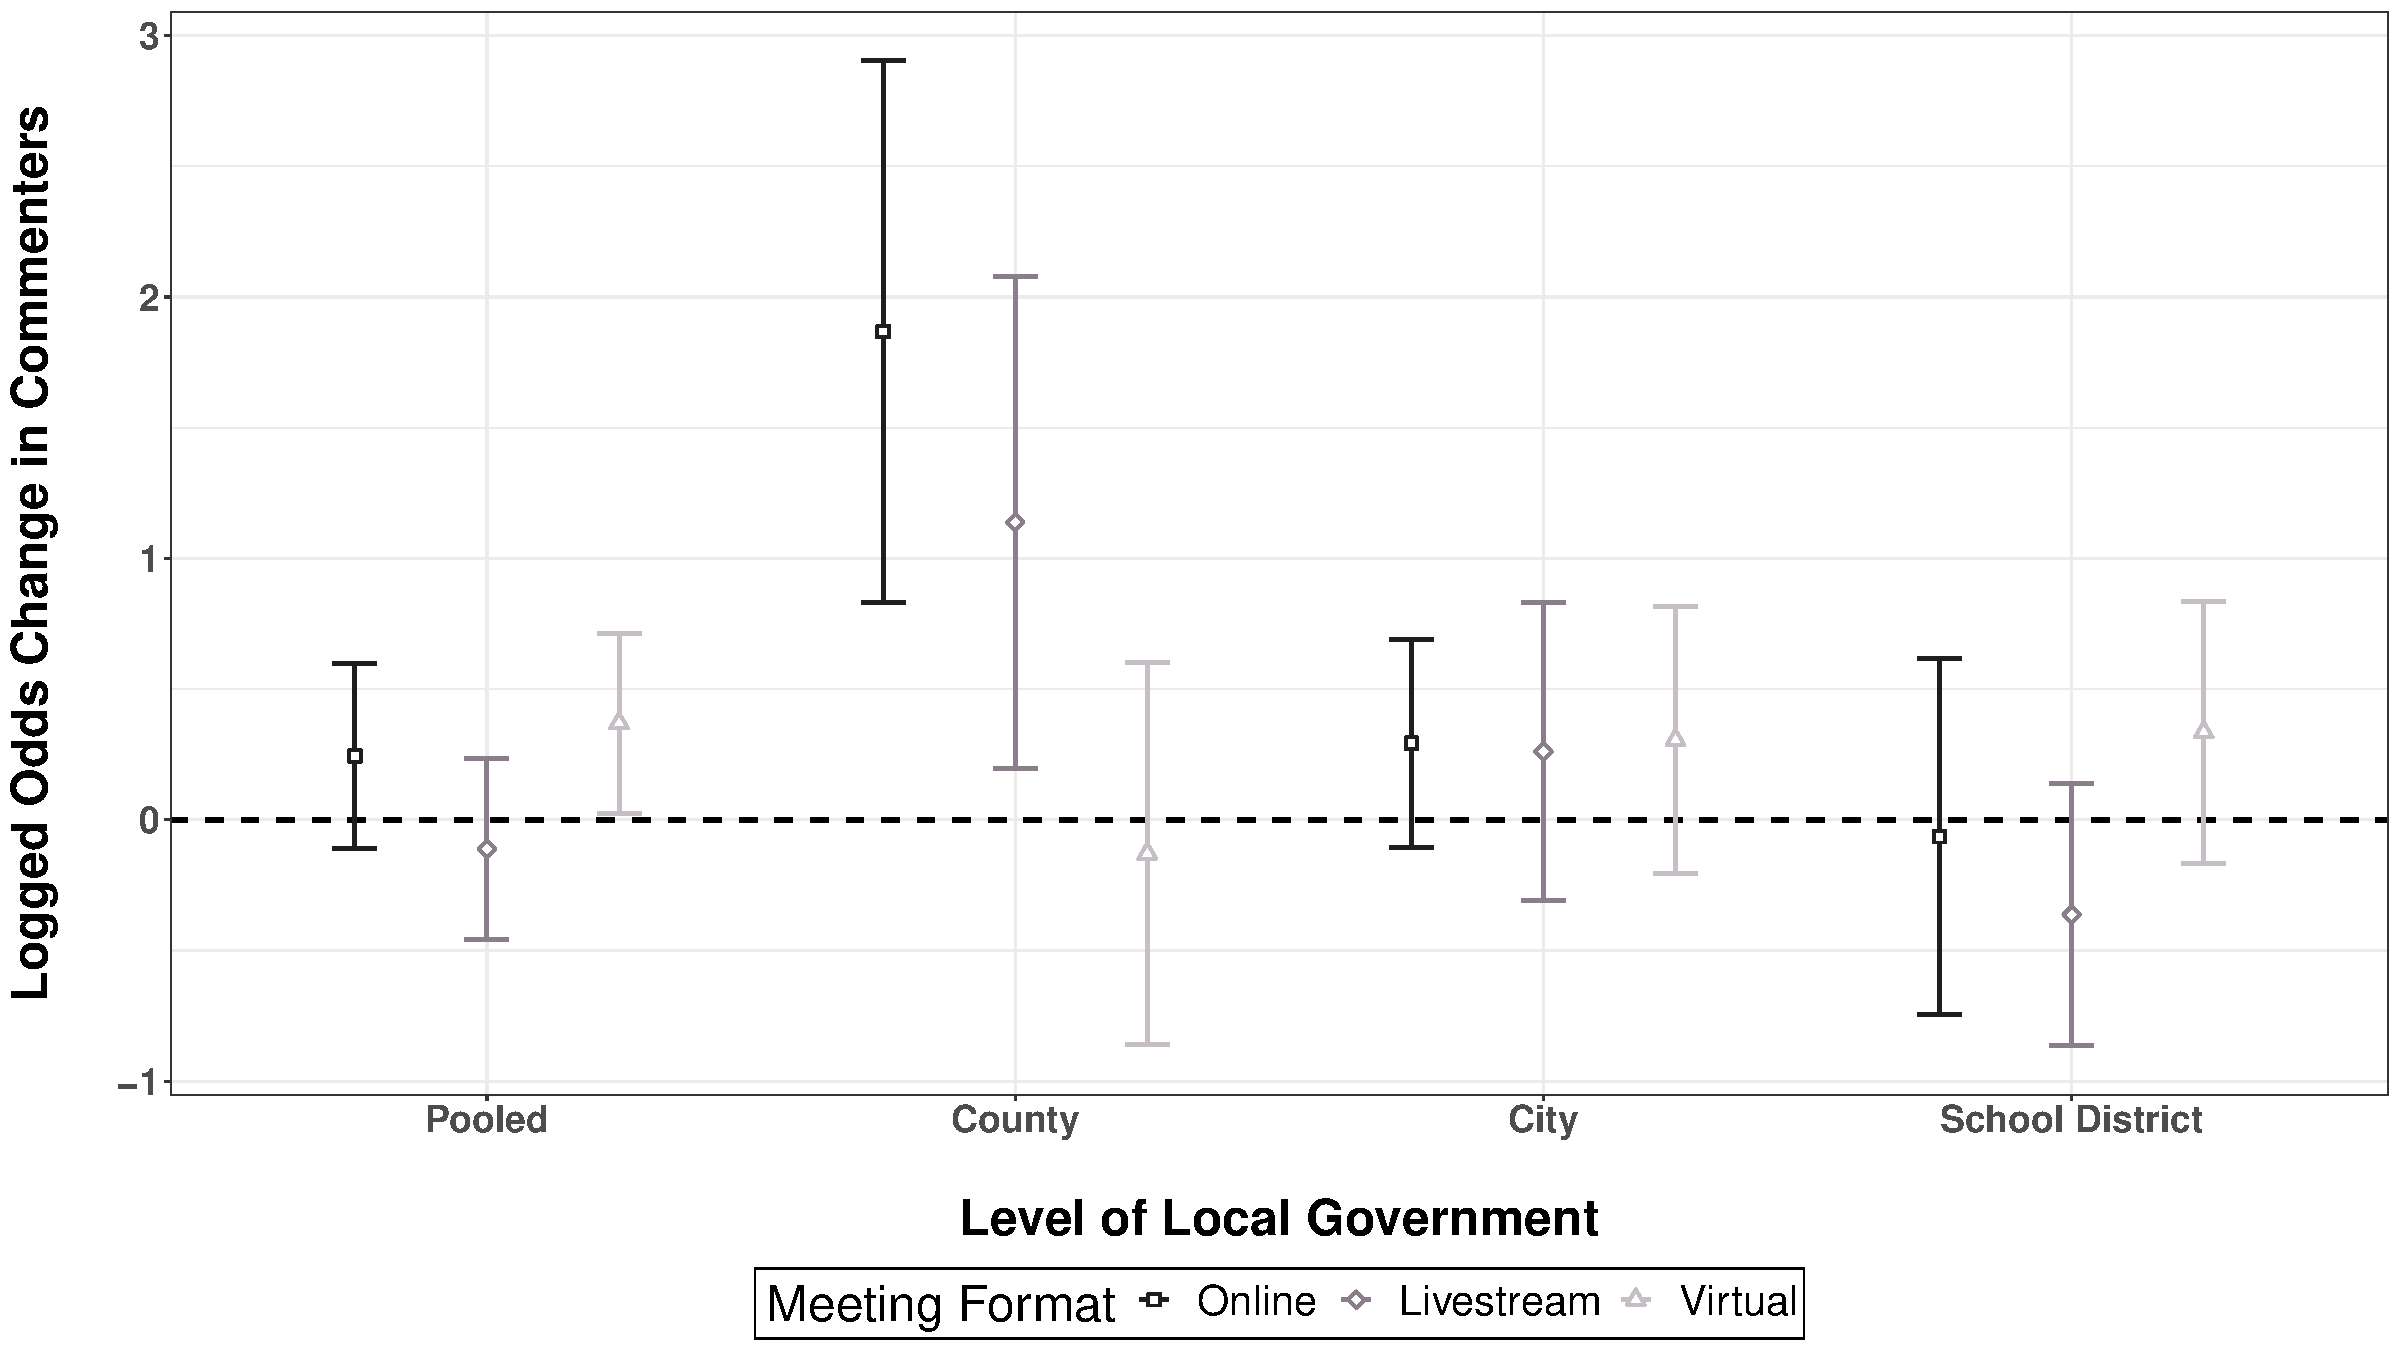
\includegraphics[scale=0.41]{Figures/MainDID.pdf}
        \caption[Effect of Meeting Format on Public Meeting Participation]{\footnotesize{Full regression results are available within the Appendix}}
        \label{fig:MainDID}
    \end{figure}

    \autoref{fig:MainDID} presents the estimated coefficients of virtual, livestreamed, and online meeting formats from my pooled and government-level models. For the pooled model, only the virtual meeting coefficient appears positive and statistically significant, with a value of 0.368. This estimate translates to a sizeable 45\% increase in the average monthly commenters or roughly 2-3 additional commenters per month.\footnote{These effects appear robust to alternative modeling strategies such as lagged dependent variable regression and the inclusion of government-level fixed effects. However, the effects lose significance but maintain direction when using more robust estimation strategies such as \citet{imaiUseTwoWayFixed2021}'s weighted linear fixed effects model.} While seemingly minor, these additional commenters could have a significant impact given the smaller scale and the increased individual political efficacy of local democracy \citep{oliverLocalElectionsPolitics2012}. Virtual meetings appear unique in their effect on meeting participation. Both online and livestreamed meetings appear not to significantly affect meeting participation. Intuitively this makes sense as virtual meetings allow individuals to participate without having to submit their comments ahead of time or physically attend. This added flexibility likely overcomes the traditional costs of meeting participation. Additionally, virtual meetings' capacity for deliberation may make participation more appealing and foster increased commenting \citep{collinsDoesMeetingStyle2021}. Interestingly, the coefficient surrounding livestreamed meetings is negative, albeit not significant. This potentially negative result could be due to livestreamed meetings' potential as a substitution rather than a promotion of meeting participation. Individuals can theoretically watch local discussions without having to participate themselves and voice their concerns only if they are not appropriately addressed within the meeting. Pooled together I find evidence that virtual meetings, in particular, fostered additional participation within local meetings, but the effect of these meetings may change between levels of local government as they vary in size and scope. 

    For the county model, livestreamed and online meetings appear to significantly increase meeting participation with coefficients of 1.139 and 1.868, respectively. Virtual meetings alone did not significantly affect meeting participation for the county. These abnormally large and significant coefficients translate to increases in meeting participants of 212\% for livestreamed meetings and 547\% for online meetings in general. Counties are geographically larger and serve more expansive constituencies; thus, they may benefit most from the added accessibility of online meetings.  Whether meeting accessibility is the sole cause of these large effects, however, is unlikely. Given the county model’s reduced form, within year time-varying confounders—namely the spread of the COVID-19 virus and discussions of racial inequities in policing—likely inflate the estimates. Examining the contents of the meeting minutes confirms this suspicion. Both meetings in which the county experienced the greatest number of participants involved discussions on reopening schools during the pandemic and the continuation of the county’s mask mandate. These meetings alone drew over 2,500 comments from citizens, far above the average 49 the county tended to receive before then. The simple fact that so many citizens \emph{could} participate may be evidence enough that accessibility matters for participation in county meetings, even if their exact causal impact is beyond the design of my simplified model.

    Turning to the city and school board models, the effects of online meetings become muddled. Online meetings of either kind do not significantly influence participation. The effect of virtual meetings is in the same direction as both the pooled and county models, but the effects of livestreamed and overall online meetings point in opposite directions for each level of government. These null effects may suggest that for these smaller governments, accessibility may matter far less than other political factors. While online meetings may remove the burden of participating in meetings, individuals may not have a reason to attend these meetings or are not engaged in local events \citep{hopkinsIncreasinglyUnitedStates2018}. Given that I find significant effects at the aggregate level, data restrictions may also be to blame as my dataset does not include enough local governments to detect the potentially nuanced effects surrounding meeting accessibility. Another possibility for the difference in effects between local government levels is that online meetings impacted some local governments and not others.

    \subsection{Did Accessibility Have Differential Effects?}
    Could online meetings affect local governments differently depending on their individual characteristics? Government and community norms may shape engagement and moderate the effects of online meetings \citep[e.g.,][]{choExperimentingPublicEngagement2021,nuamahCloseHomePlaceBased2021}. Traditional TWFE models assume homogenous treatment effects and do not allow for group-level estimates of the average treatment effect (ATE). Instead, I turn to an alternative multi-period difference-in-difference model proposed by \citet{callawayDifferenceinDifferencesMultipleTime2021}. This alternative model provides two key benefits beyond the traditional TWFE design. First, it allows for heterogenous treatment effects between groups and can estimate a separate ATE for each government in my sample.\footnote{Small groups can cause estimation problems for this model, so I follow the authors' advice and average the ATE for each group across all time periods in which they are treated.} Thus, I can estimate the effects of online meetings based on when individual (or groups of) local government(s) switch away from online meetings. Second, the model allows for the staggered adoption of treatment and therefore avoids the potential inferential concerns which can occur when applying traditional TWFE models to multi-period difference-in-difference designs \citep{imaiUseTwoWayFixed2021,sunEstimatingDynamicTreatment2021}.

    Notably, the model does require that once a unit is treated, it remains treated for the remainder of the data. Thus, I alter my previous design and leverage that all local governments had to hold some form of online meeting following the Stay Home Missouri order. In doing so, I effectively flip my treatment indicator and examine the effect of switching \emph{away} from online meetings.\footnote{No government in my sample switched back to online meetings after switching away from them.} If online meetings \emph{increase} participation, then I should find \emph{negative} treatment effects as local governments effectively lose participation by switching back to offline meetings. To leverage all possible changes in meeting accessibility, I estimate the effect of entirely switching away from online meetings and the effects of switching away from only virtual meetings. Given my focus on heterogeneous effects within local government, I estimate separate models for city and school board governments. One last assumption of the model is that units do not anticipate treatment or at least have limited anticipation of it. Local governments could theoretically anticipate switching away from online meetings and notify their constituencies, thus influencing the total number of commenters. This anticipation would bias my results and cause the estimator to become inconsistent. However, I find no evidence of anticipation when examining various lags and leads of treatment or the inclusion of various anticipation terms.

    \begin{figure}[H]
        \centering
         \text{Effect of Switching Away From Accessible Meetings By School Board Groups}\par\medskip
        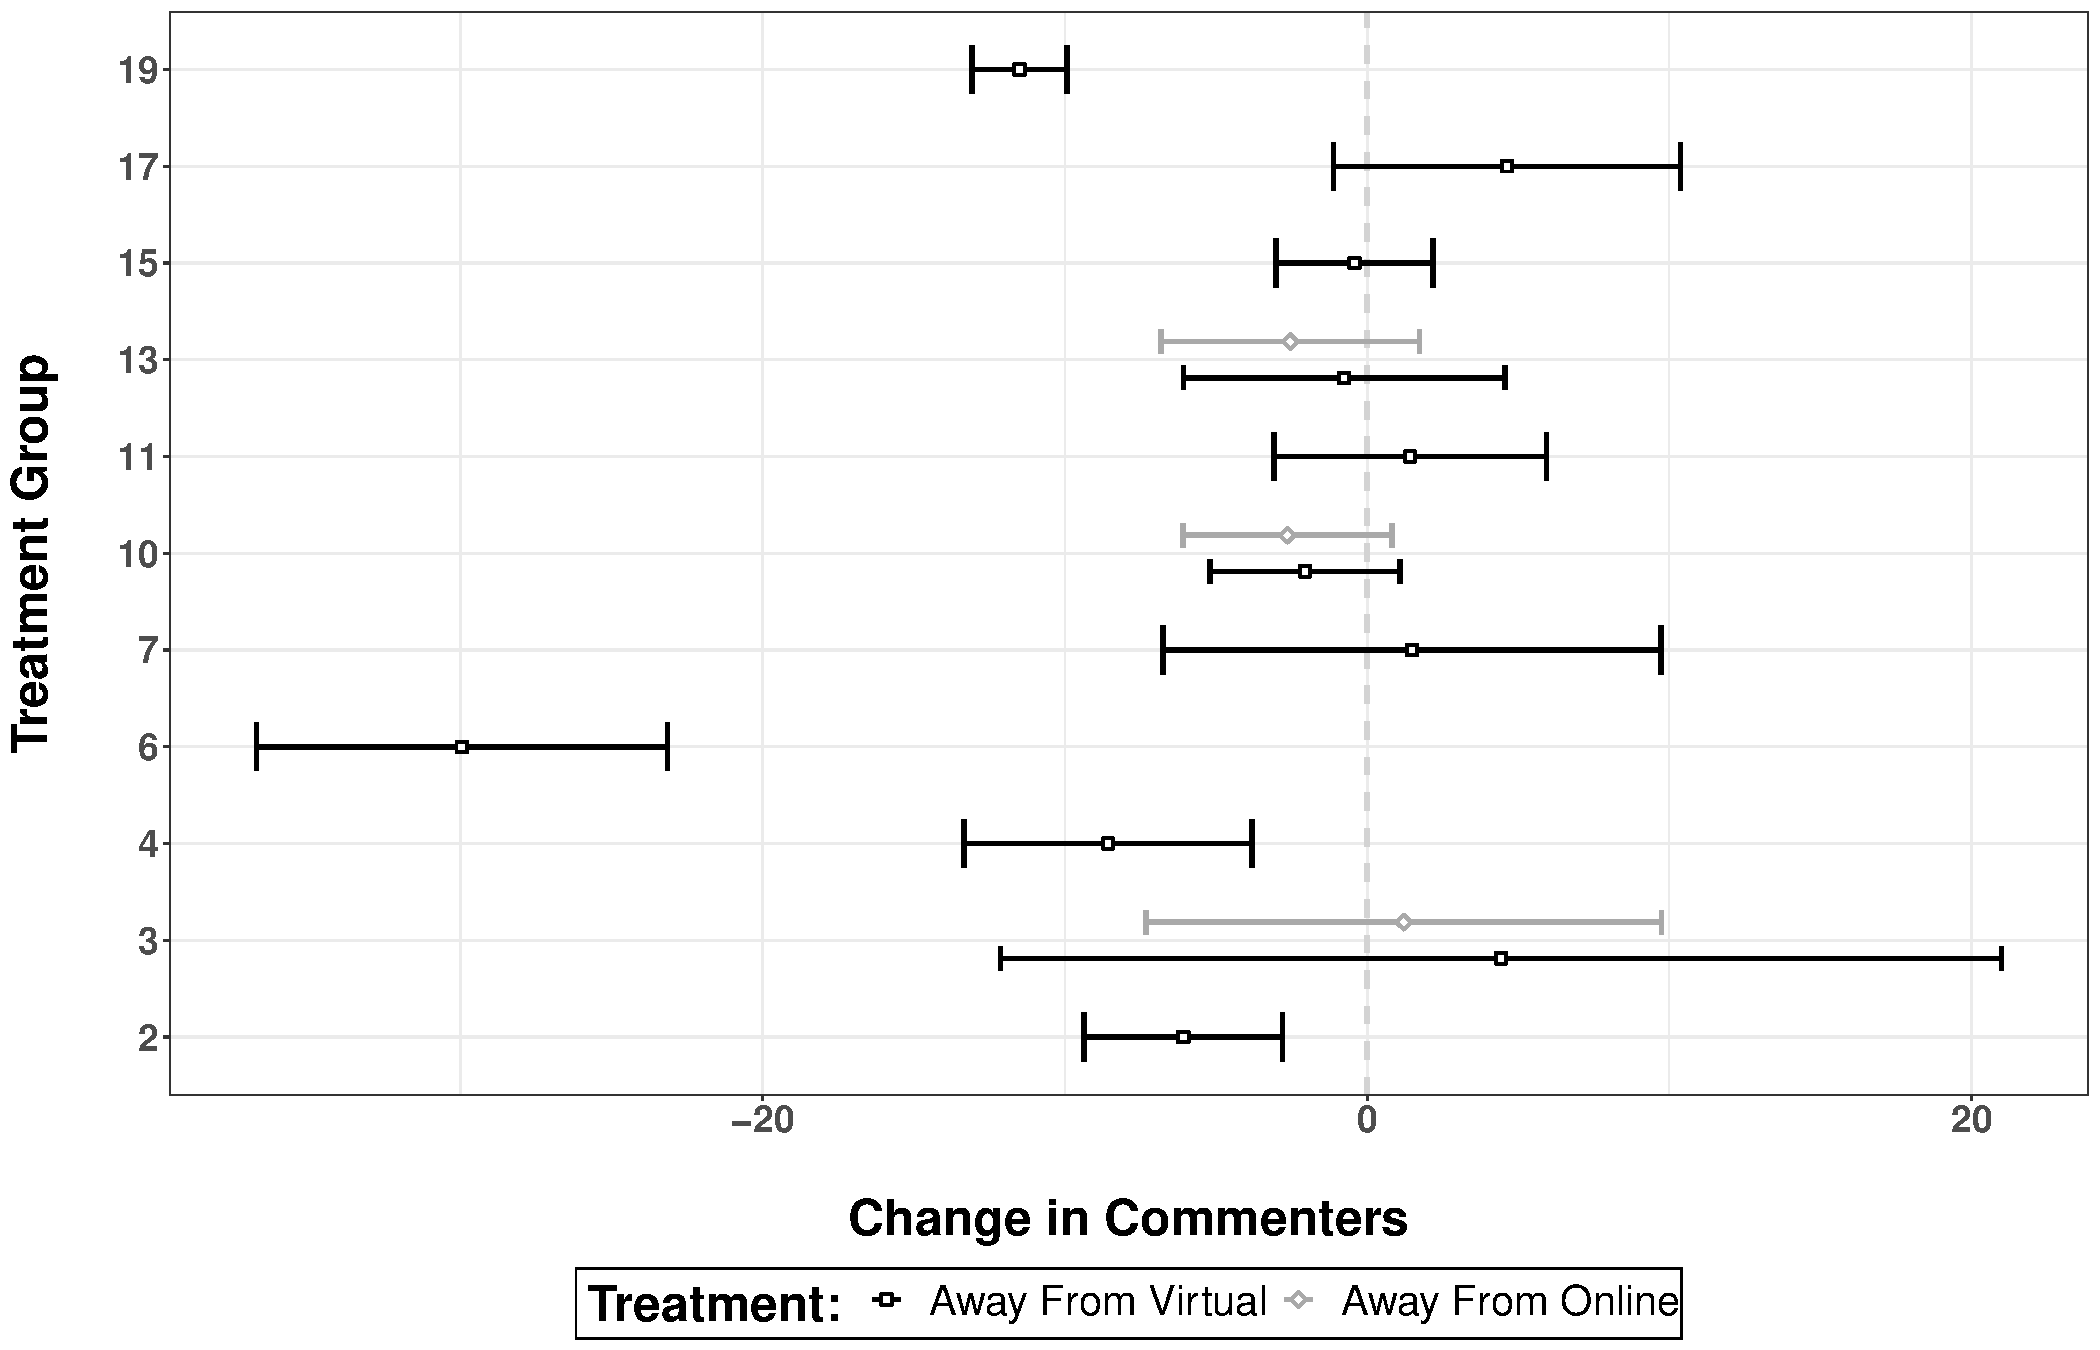
\includegraphics[scale=0.39]{Figures/SchoolMPDID.pdf}
        \caption[Effect of Switching Away From Accessible Meetings By School Board Groups]{\footnotesize{Effects are calculated using multi-period difference-in-difference design. X-axis indicates the ATE for a group averaged across all treated periods. Y-axis indicates the treatment group and the number of months passed before treatment. Standard errors are doubly robust and clustered at the group level.}}
        \label{fig:AwaySchool}
    \end{figure}

    \autoref{fig:AwaySchool} and \autoref{fig:AwayCity} present the differential effects of switching away from online meetings for cities and school boards within my sample. The y-axis indicates the treatment group and the number of months before it was treated. For example, group two in \autoref{fig:AwaySchool} switched away from virtual meetings two months after the Stay Home Missouri order started. Across both models, all but two groups consisted of a single government. The x-axis captures the group specific ATE in the change of monthly commenters. Immediately apparent, virtual meetings appeared to have differential effects within and between school boards and city governments. Most school boards saw no change in their number of monthly commenters. However, three experienced significant losses in meeting participation after switching away from virtual meetings, with one school board experiencing an estimated decline of 29 monthly commenters. The opposite appears true for cities. Most cities similarly experienced no change in their average monthly commenters; however, in the case of two cities, switching away from online meetings had a positive and significant effect on meeting participation. For these cities, switching away from online meetings increased their monthly commenters by roughly a single additional commenter.

    \begin{figure}[H]
        \centering
         \text{Effect of Switching Away From Accessible Meetings By City Groups}\par\medskip
        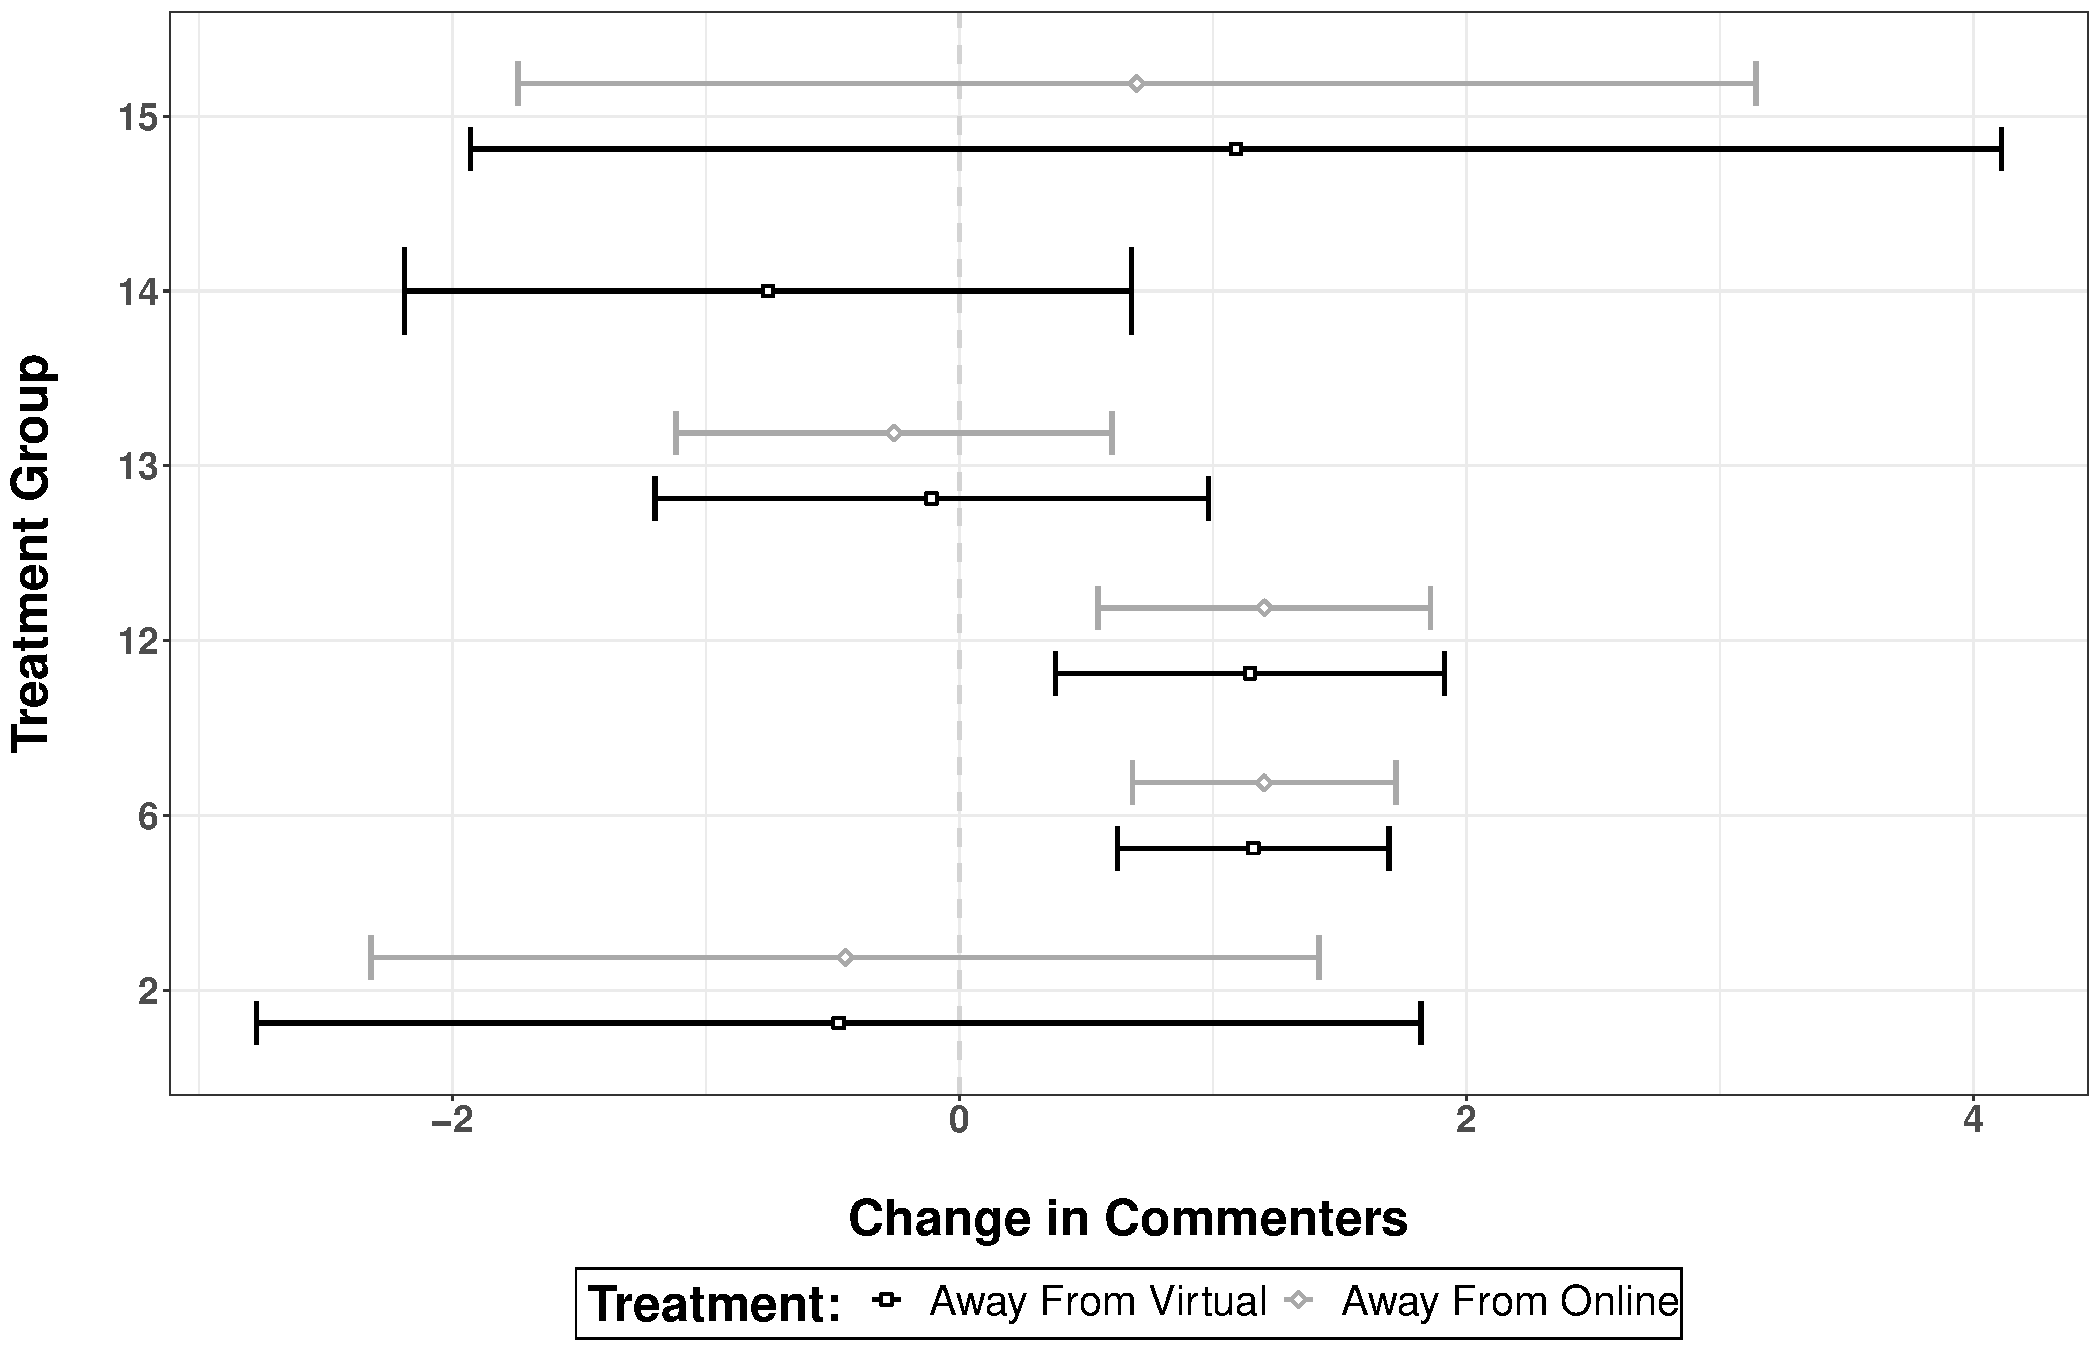
\includegraphics[scale=0.39]{Figures/CityMPDID.pdf}
        \caption[Effect of Switching Away From Accessible Meetings By City Groups]{\footnotesize{Effects are calculated using multi-period difference-in-difference design. X-axis indicates the ATE for a group averaged across all treated periods. Y-axis indicates the treatment group and the number of months passed before treatment. Standard errors are doubly robust and clustered at the group level.}}
        \label{fig:AwayCity}
    \end{figure}

    Beyond group-level estimates of the effect of online meetings, these models can also provide additional insight regarding the effect on cities and school boards as a whole. Following \citet{callawayDifferenceinDifferencesMultipleTime2021}, I average the group-level effects to obtain overall estimates of the ATE. Doing so provides a significant effect of -4.30 for school boards switching away from virtual meetings and a non-significant effect of -1.3 for switching away from online meetings altogether. For cities, both the effect of switching away from virtual meetings (0.324) and online meetings (0.32) appear positive but not significant. While the effect of virtual meetings contrasts those found within the school specific TWFE model, it is similar in size to the estimated effects found within the pooled model. 
    
    Since I group governments by treatment timing, I also can examine how said timing may influence the effects of online meetings. Theoretically, how quickly a government switches away from online meetings may moderate their experience as citizens and public officials have varying amounts of time to become familiar with the new meeting styles. In the case of both school boards and cities, I find some evidence that those governments who switch sooner experience more significant changes, but the effect appears to be inconsistent. Not accounting for those with null effects, school boards who switched away from virtual meetings 2-4 months after the Stay Home Missouri order experienced roughly the same participation loss as those who switched a year later. No apparent pattern exists for cities changing away from virtual or all online meetings. These findings suggest that the effects of online meetings are likely more centered on individual government characteristics rather than the timing of their choice to switch.

    Overall, this evidence, combined with that of my primary models, suggests that meeting accessibility positively affected participation within local democracy. However, this boost was inconsistent across and within levels of local government. Some governments experienced a drastic increase in participants, while others experienced no change or a slight decline. Given this potential for increased participation, it is essential to understand whether accessibility brings diverse voices or further instills pre-existing inequities in local participation.

\section{Do Online Meetings Lead to More Diverse Participants?}

\subsection{Obtaining Commenter Characteristics:}
In the previous section, I found that more accessible meetings can foster increased participation, albeit the effect varies across local contexts. Are these meetings bringing new voices to local meetings or instilling previous inequities in participation? To answer this question, I match each commenter in my dataset to a commercial voter file provided by L2. This file contains both previous records of political activity and demographic estimates for each individual. I utilize the \texttt{fastLink} package in R to probabilistically match commenters on first name, last name, and address \citep{enamoradoUsingProbabilisticModel2019}. While probabilistically matching commenters can lead to higher rates of false positive matchings in which I incorrectly match commenters to voters, it decreases rates of false negatives and increases my overall match rate. The process also allows me to include measures of matching uncertainty within my later analyses. Given the voter file holds more than 650,000 records for the St. Louis region alone, I block voters first on government boundaries and then on zip code.\footnote{When matching county commenters, I only block voters based on zip code} This process aims to narrow down the universe of possible matches and improve matching rates. I follow previous work matching commenters to administrative records and match commenters with a match threshold of 0.85 \citep{yoderDoesPropertyOwnership2020}. In other words, two records are considered a match if the posterior probability of said match is greater than 85\%. Before examining whether online meetings encouraged diverse meeting participation, my sample provides a novel opportunity to characterize commenters across local contexts.


\subsection{Characterizing Commenters Across Local Contexts}
\autoref{fig:CommentDemo} displays the difference in means between commenters and all voters living within the region. For this initial analysis, I pool commenters across all meeting formats. Regarding school boards and cities, I subset to only voters residing within the jurisdiction of my sample. To account for the uncertainty in my matching procedure, I down-weight each estimate by my match threshold (0.85) as prescribed by \citet{enamoradoUsingProbabilisticModel2019}. Previous studies of commenting within municipal politics find that individuals who comment are whiter, weather, older, and more likely to be homeowners than their immediate communities \citep{einsteinWhoParticipatesLocal2019,yoderDoesPropertyOwnership2020}. I find broadly consistent findings when examining cities in my sample. City commenters stand out as predominantly whiter and older, with a higher likelihood of being homeowners and actively participating in national and local elections. Interestingly, I do not find a significant overrepresentation of men as consistently documented in previous studies \citep[e.g,][]{einsteinStillMutedLimited2022}, albeit the coefficient is in the same direction.

\begin{figure}[H]
    \centering
     \text{Difference Between Voters and Commenters}\par\medskip
    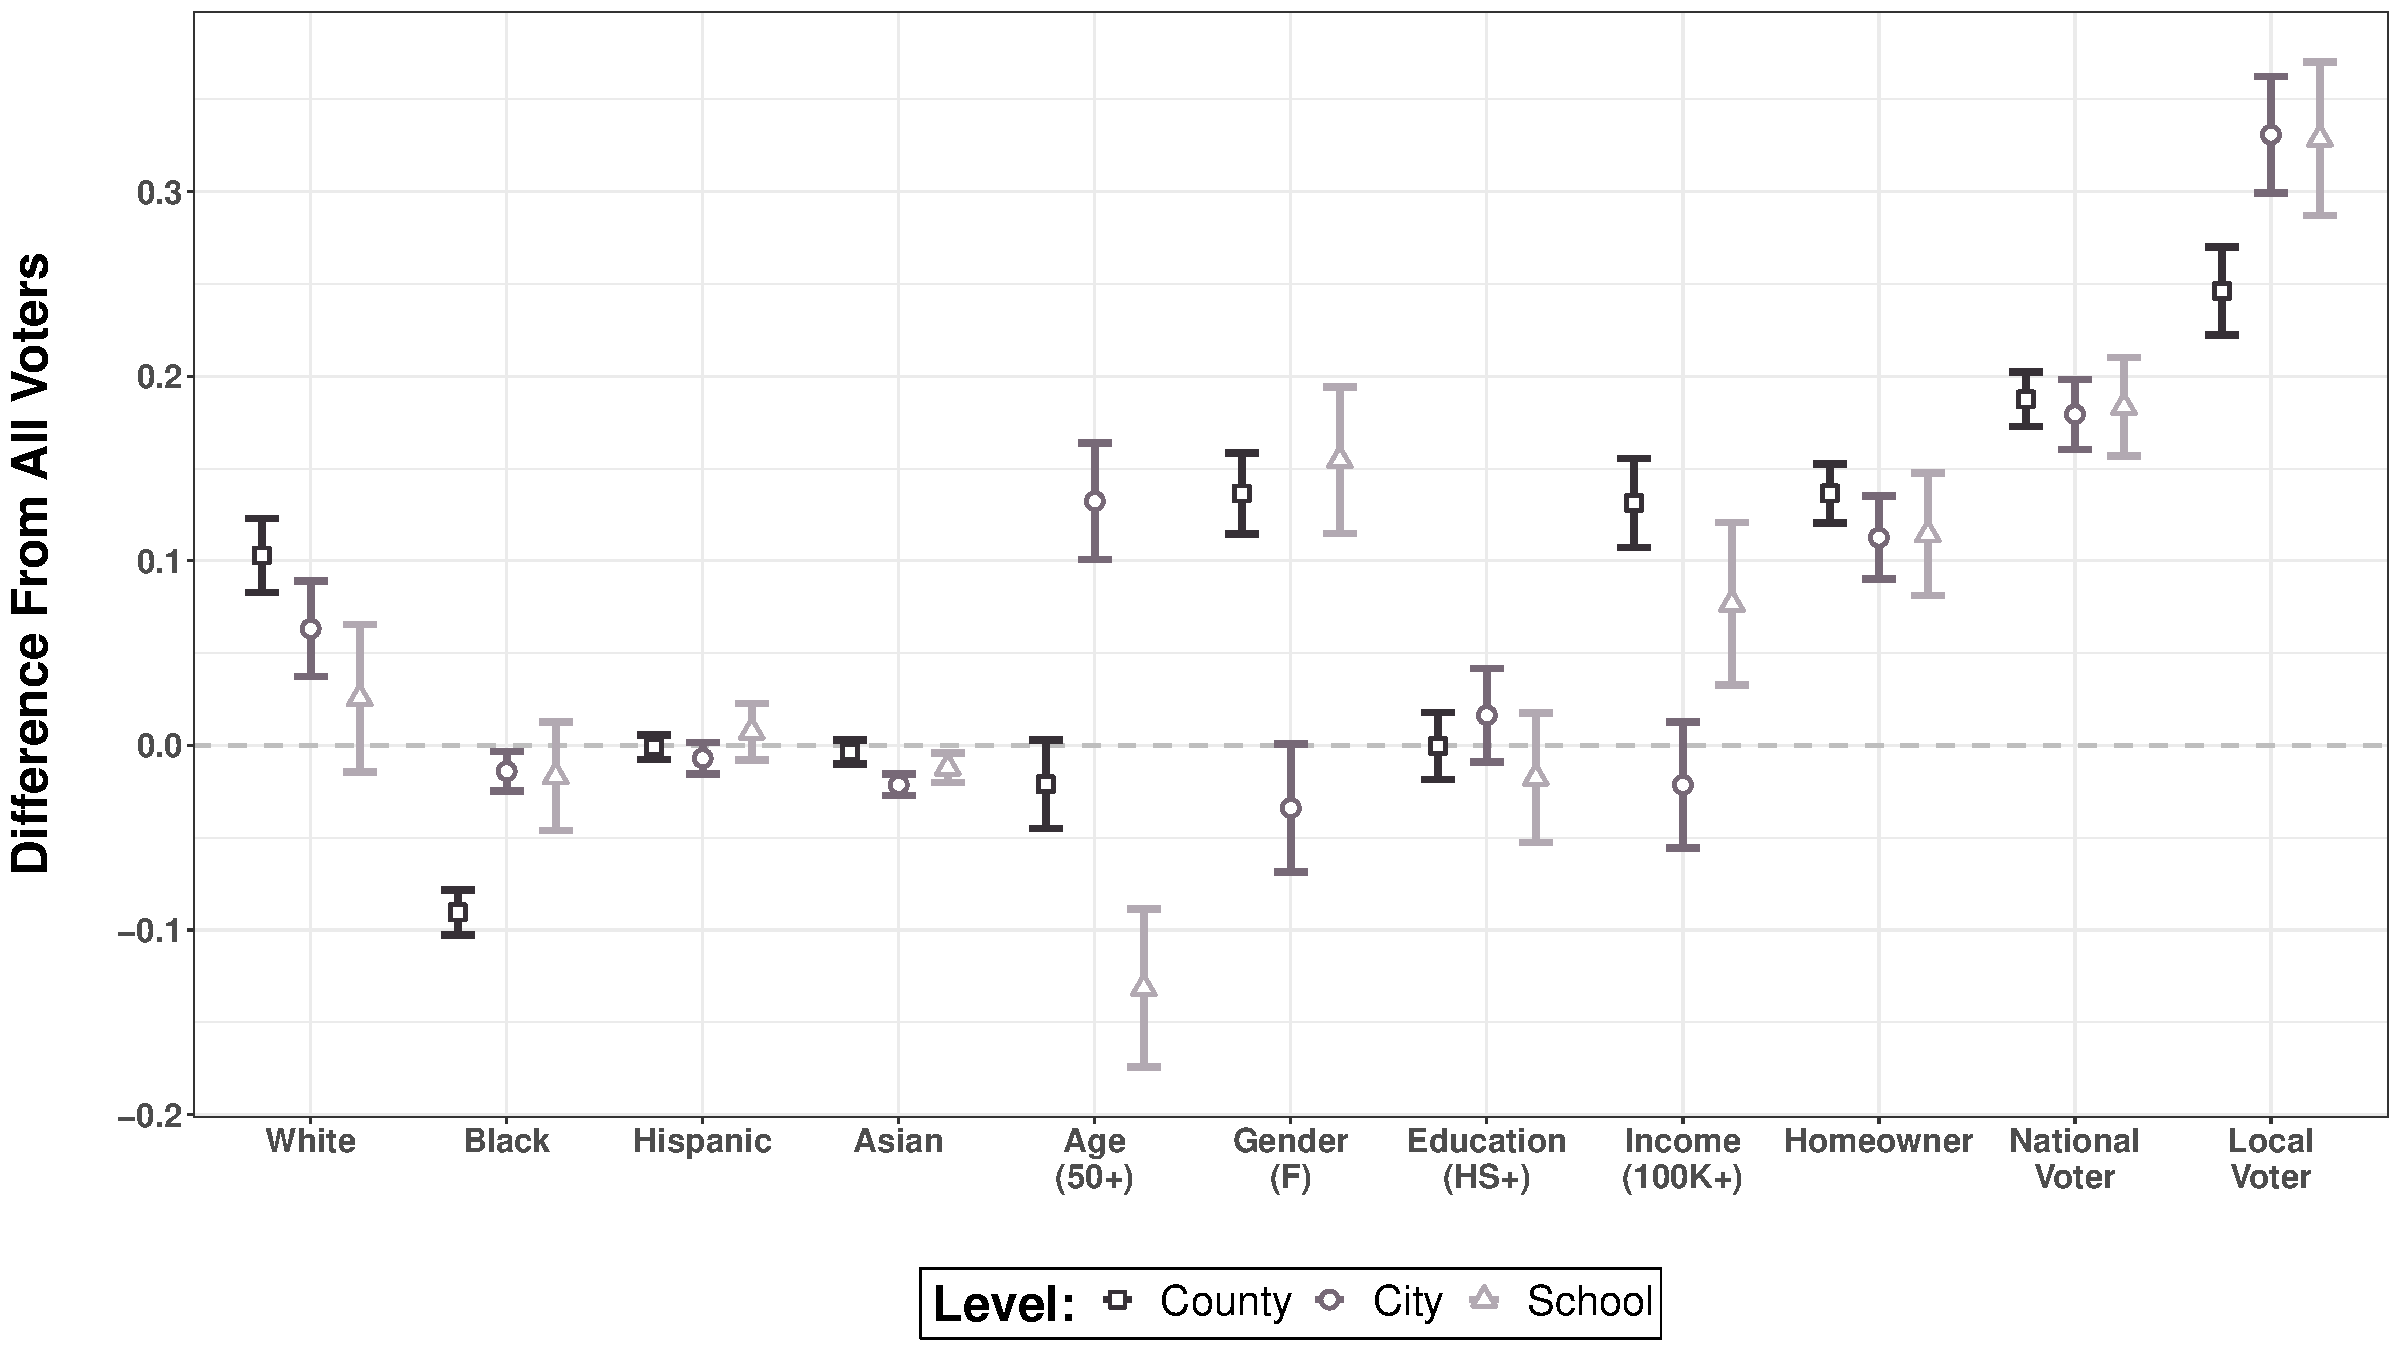
\includegraphics[scale=0.41]{Figures/CommentDemoPooled.pdf}
    \caption[Difference Between Voters and Commenters]{\footnotesize{Commenters are pooled across all meeting formats. School and city comparisons are subset to their repective voters. Simultaneous comparisons are available in the Appendix.}}
    \label{fig:CommentDemo}
\end{figure}

County governments deal with inherently different issues and represent larger constituencies; however, they are still comparable to local governments in terms of services and powers. When examining the differences between county commenters and their surrounding communities, I find that they also suffer from similar participation inequities as in municipal politics, albeit with several key differences. Commenters are similarly whiter and wealthier, with a higher likelihood of being homeowners and politically active but are not so different from their communities regarding education or age. One of the most surprising differences is that significantly more women comment at the county level. These effects may be due to counties handling issues related to health and welfare, two policy areas women lawmakers are more likely to prioritize \citep[e.g., ][]{huddyConsequencesGenderStereotypes1993, voldenWomenIssuesTheir2018, paysonDecomposingSourceGender2023}. Additionally, the pandemic's gender-specific impacts may have motivated women to participate at greater rates \citep{carrerasWhoDoesCaring2023,johnsonGenderPoliticalLeadership2020}. I find similarly high rates of women participating in school board meetings.

Commenters at school board meetings are younger and more likely to be women than their surrounding communities. Intuitively this makes sense, given the traditional and gendered role women tend to hold within households, and younger individuals are more likely to have school-age children. Thus, these two groups are more likely to have a vested interest in school board outcomes. These gendered effects, in particular, provide a new perspective on the difference in gendered political participation within local politics \citep{coffeSameGameDifferent2010}. Importantly they highlight yet another dimension along which the pandemic potentially impacted genders differently. Along other demographics, school commenters appear to vary from their communities in unique ways. While commenters are more likely to be wealthier, own homes, and vote in recent elections, they do not differ significantly in terms of race. Surprisingly, school board commenters largely resemble the racial makeup of their surrounding communities. This lack of difference may be partly due to the well-documented mobilization of minority communities to protect school resources \citep{morelTakeoverRaceEducation2018,nuamahCloseHomePlaceBased2021,kitchensExitInvestSegregation2021}. However, this seemingly equal participation in public meetings may come at an increased cost of participation paid on behalf of Black individuals especially \citep[see][]{nuamahCostParticipatingPoor2021}. Overall, school board, county, and city commenters appear significantly different from their surrounding communities but do so uniquely depending on the local context and policy priority of the local government.


\subsection{Measuring the Difference Between Online and Offline Commenters}

Online meetings should, in theory, lessen the burdens of political participation faced by different groups and potentially increase the diversity of commenters. However, previous work examining online meetings in the context of planning and zoning meetings has found them to largely attract the same demographics and fail to address inequities in meeting participation \citep{einsteinStillMutedLimited2022}. To examine the effects of online meetings across my sample, I calculate the difference in means between online and offline commenters relative to all voters living within my sample’s geographic coverage. Doing so allows me to compare commenters to those from alternative meeting formats as well as their communities. \autoref{fig:OnOffDemo} displays the difference means between each group, again adjusted by my match uncertainty.

\begin{figure}[H]
    \centering
     \text{Difference Between Voters and Commenters By Meeting Format}\par\medskip
    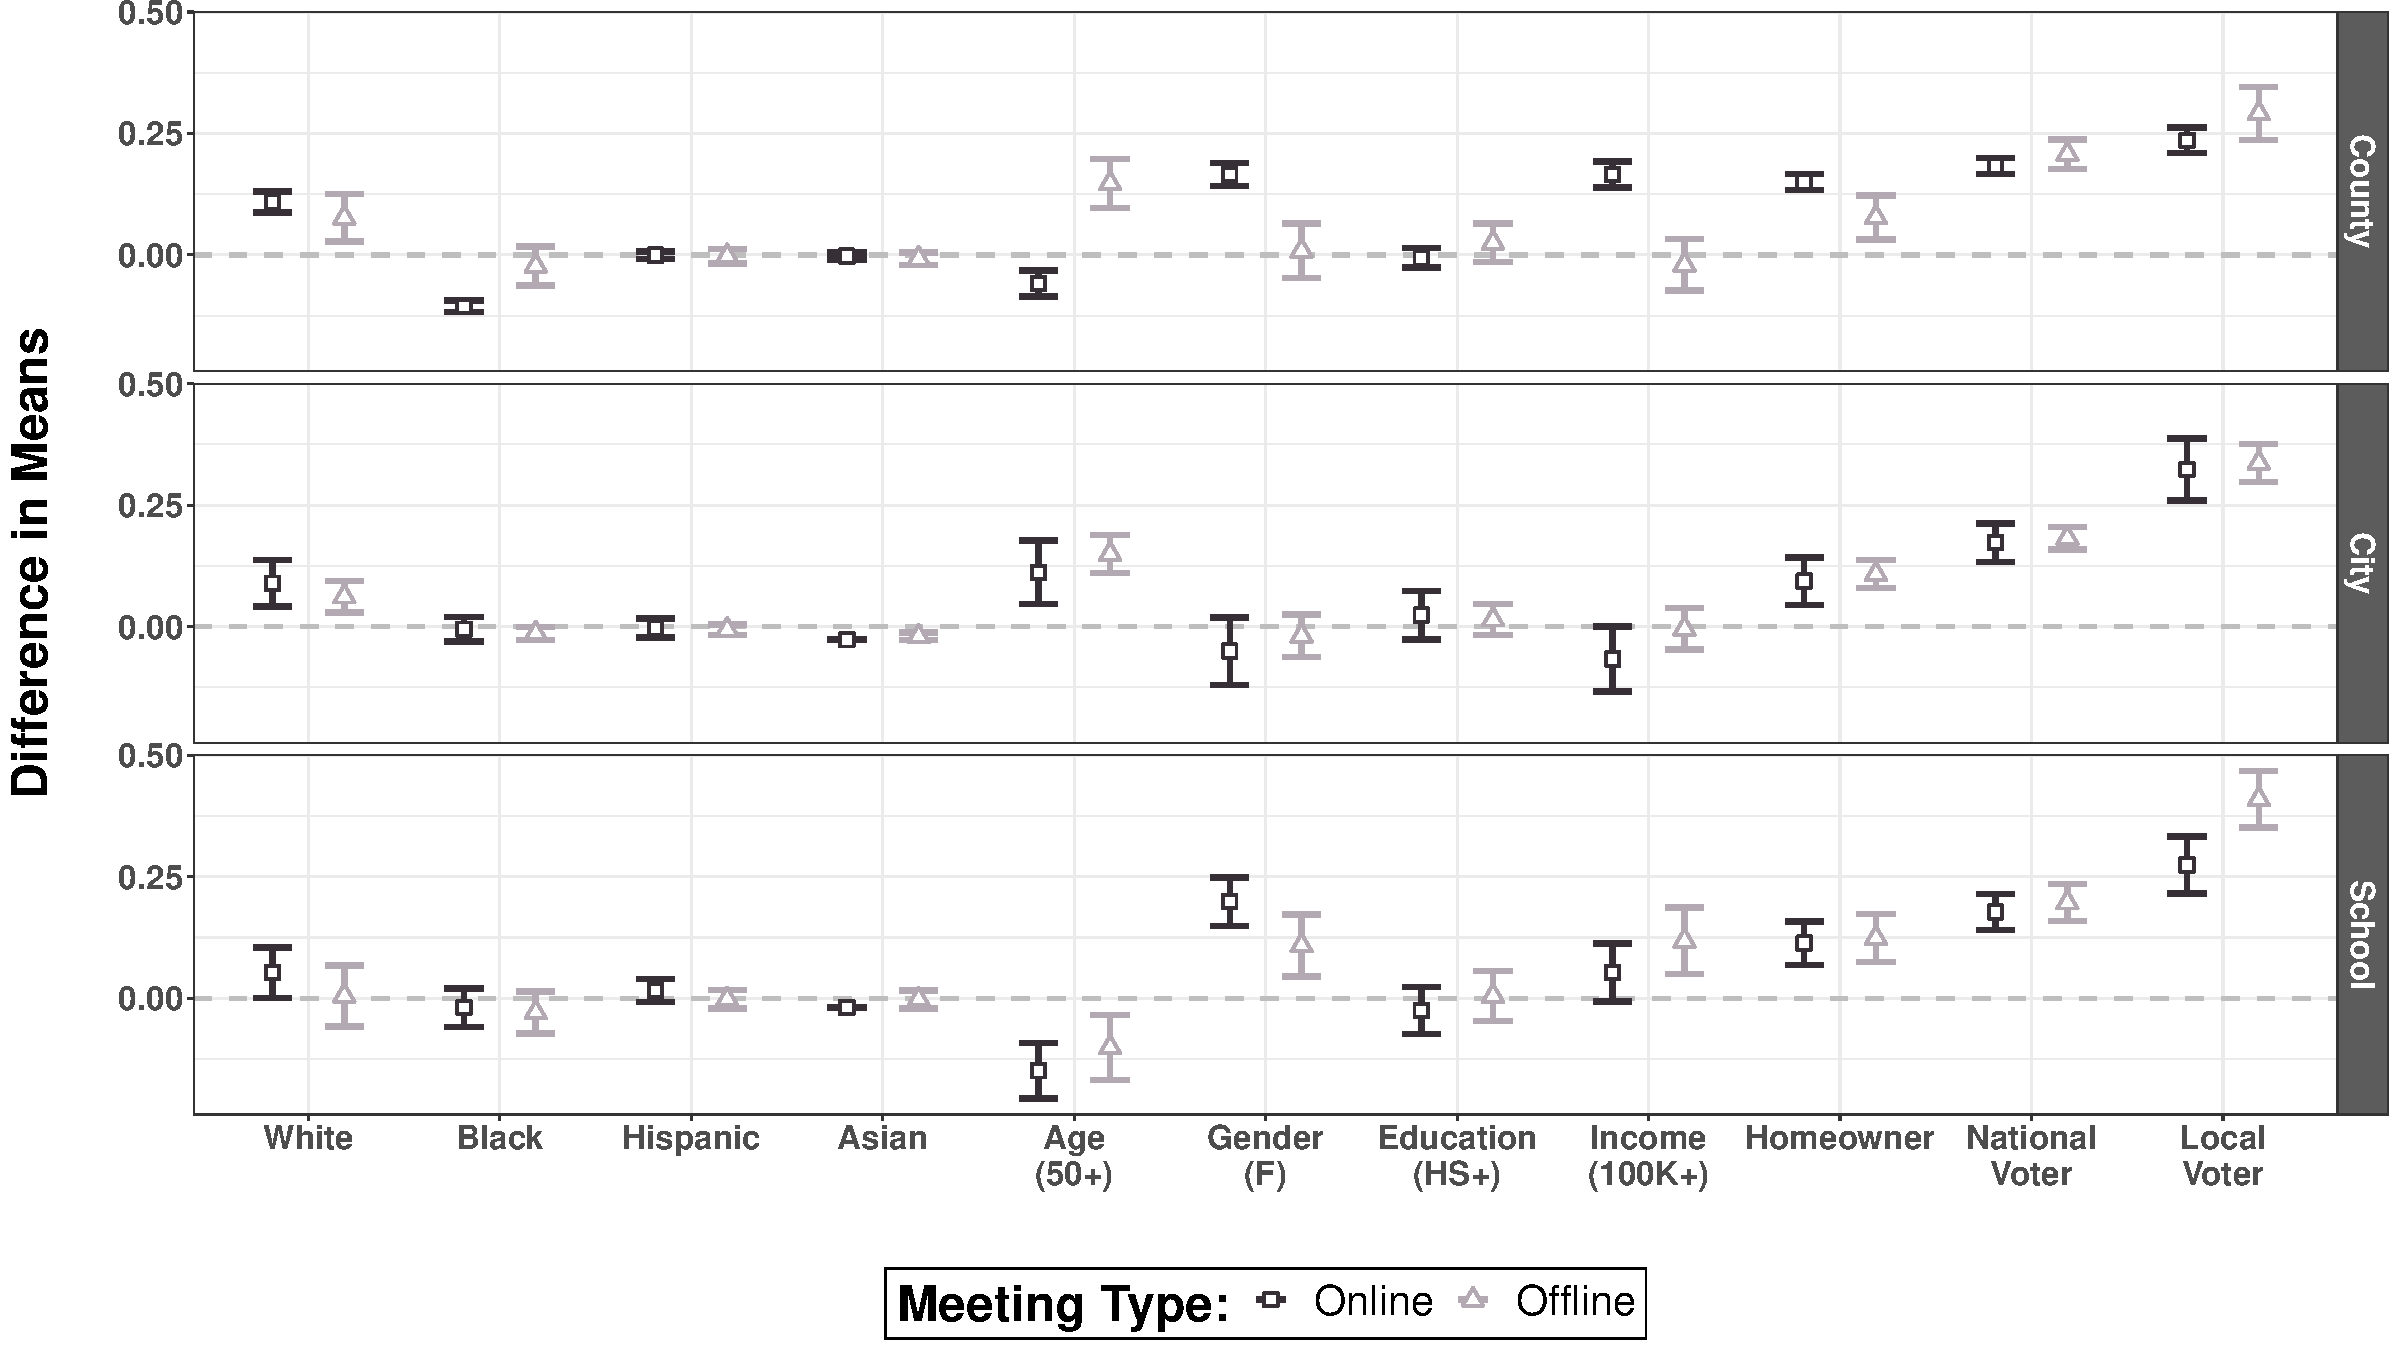
\includegraphics[scale=0.45]{Figures/OnOffDemoComparison.pdf}
    \caption[Difference Between Voters and Commenters By Meeting Format]{\footnotesize{School and city comparisons are subset to their repective  voters. Estimates are adjusted to account for uncertainty in the matching process. Simultaneous comparisons are available in the Appendix.}}
    \label{fig:OnOffDemo}
\end{figure}

Overall, online commenters across all three local contexts are similar to their offline counterparts. They tend to be misrepresentative of their communities along dimensions of race, income, and political engagement. For the county, online meetings did attract significantly more women and younger commenters. Online meetings, in particular, appear responsible for the over-representation of women identified in my pooled analysis above. However, these benefits came at the cost of widened gaps in racial representation, income, and homeownership. In the case of cities, I document no noticeable change between online and offline commenters, with results similar to \citet{einsteinStillMutedLimited2022} examination of online meetings. Finally, for school boards, online meetings attracted more individuals previously not engaged in local elections and potentially lessened the divide in income, albeit the estimate is not statistically distinguishable from that of offline commenters. Beyond these characteristics, I find no substantial differences between online and offline school board commenters.

Despite the theoretical benefits of online meetings, I find they had a mixed effect on the diversity of meeting participants. For the county and school boards in my sample, online meetings lessened some divides and incentivized an over-representation of traditionally underrepresented groups; however, many previous inequities in participation persisted within these meetings. Online meetings appeared even to exacerbate some disparities in the county's case. Notably, my approach above does not account for time or geographic varying confounders, which may alter specific demographics' propensity to comment. To partially address this concern, I utilize a logistic regression to examine differences between online and offline commenters simultaneously with added geographic controls. I present the results within the Appendix and find substantively similar results.

\section{Discussion:}
Online meetings were adopted out of necessity in response to the pandemic but offered a potential solution to historically low engagement in local political meetings. These meetings act as a crux for local democracy and allow individuals a direct connection to local public officials and policy-making processes. Given historic inequities in who attends and the resulting policy outcomes, increasing the quantity and diversity of meeting participants is vital to the healthy functioning of local democracy. Utilizing a novel dataset of meeting commenters, I find that online meetings are an effective tool to expand access to local governments, but in isolation, they are insufficient to address pre-existing inequities in who participates within local democracy. What’s more, I find that inequities in participation previously found within municipal politics are present within both county and school board contexts. However, I find some silver lining for local democracy as some groups—namely women—appear to be overrepresented within some levels of local politics. This finding suggests that some groups may effectively make up for underrepresentation in local politics by being overly active in other potentially more relevant local contexts. Future work should explore whether these potential increases in participation manifest into meaningful policy change for these often-underrepresented groups.

For policymakers, these results bring mixed news. On one hand, accessibility matters for local government and can boost the number of voices heard within local meetings. What’s more these voices at least appear to be sincere. Section A.4 of Appendix I shows evidence that online participants share jurisdictionally relevant comments and, contrary to fears of trolling or increased incivility, do so with a similarly positive sentiment as their offline counterparts. However, improving access is no panacea for the deep-rooted inequities present within local politics. In fact, improving accessibility, when implemented alone, may do more harm than good by exacerbating existing inequities in political participation. To truly address these problems, policymakers likely need to find a way to empower individuals and their communities and improve their sense of political efficacy. If individuals do not believe their voice can impact local policy outcomes, allowing them to attend virtually will likely not persuade them to participate. 

\chapter{Is it All Good in the Neighborhood? How Partisanship May Shape Evaluations of Municipal Services}
\label{chap:chapter2}

While extensive work has been done examining how voters evaluate the performance of federal and state governments, comparably less attention has been paid to evaluations in the context of local governments. In what work has been done, researchers often focused on small geographical areas and how information availability shaped evaluations \citep[e.g.,][]{berryAccountabilityLocalElections2007,paysonWhenAreLocal2017}. We still know relatively little about how voters' individual-level characteristics shape how they evaluate their local governments and their respective services. Nor do we know whether these evaluations correlate to the actual performance of local governments. Traditional conceptions of local politics might suggest that these evaluations are primarily a result of voters' day-to-day interactions with these services \citep[e.g.,][]{kaufmannUrbanVoterGroup2004,yoderDoesPropertyOwnership2020}; however, this framework fails to take into account the growing role partisan identities play in voter's evaluations of government services at state and federal levels \citep{healyRetrospectiveVotingReconsidered2013}. Furthermore, the increasing nationalization of politics means local political issues are no longer as insulated from traditional partisan discourse as previously conceived \citep{hopkinsIncreasinglyUnitedStates2018}.

In this article, I attempt to further our understanding of how voters evaluate their local government's performance and the role partisan identities play in constructing these evaluations. I argue that local services can become polarized when local issues become nationalized and distinct partisan cleavages form in the national discourse. For these polarized services, partisanship becomes a powerful identity through which individuals construct their local evaluations. This partisan lens then biases assessments of these services toward their party's average position regarding the service.

To test this argument, I use a nationally representative and geographically diverse survey that asks individuals to grade two prominent local services, schools, and police. While both are primarily under the purview of local governments and receive significant political attention, they differ regarding their partisan division. Using administrative records from the Census Bureau and National Weather Service, I then match all respondents to their local governments. This matching allows me to, in addition to gathering respondent-level characteristics,  (1) account for locality-based effects that may influence a respondent's evaluation and (2) assign each respondent an objective measure of both services to isolate any form of partisan bias. 

Overall, I find a significant partisan bias in voters' evaluations of polarized services even after accounting for objective performance and prominent socio-economic features. Despite living in areas with similarly performing police agencies, Republicans systematically rate local police higher than Democrats and Independents. Notably, this bias is equivalent to a substantial change in objective outcome measures for police and the effects of income and race. While I find differences in how partisans evaluate local schools, the results are comparably small and outweighed by school performance. To test the robustness of my results, I subset my data set to only large cities to incorporate additional city-specific measures, alternative local services, and city and state levels of partisan control. I find support for my theory, and interestingly, my results suggest that the partisan bias is based on national partisan preferences rather than on party control of the government.

This research contributes to the growing literature on the role of partisanship within local politics and provides further evidence of the nationalization of American politics. Notably, my research is one of relatively few to map a geographically diverse collection of specifically local evaluations to their respective municipalities. My results highlight how local services, like national policy issues, can become polarized and susceptible to partisan biases. These partisan effects are especially problematic as they can influence an individual's evaluations more than a local service's objective performance. Additionally, these results have potential implications for the already low levels of accountability found with local politics, as voters may rely more on national opinion rather than local conditions when constructing their evaluations.



\section{The Process of Polarization}
I argue that some local services have become polarized due to the nationalization of American politics \citep{hopkinsIncreasinglyUnitedStates2018} and the adoption of services as party-owned issues. Borrowing from both the polarization \citep[e.g.,][]{levenduskyPartisanSortHow2010,sinclair2006party} and issue ownership literatures \citep[e.g.,][]{petrocikIssueOwnershipPresidential1996,egan2013partisan,green2004partisan}, I define a local service as polarized when parties hold ideologically distanced and distinctly homogeneous opinions regarding a service's intended purpose, appropriate support, and overall performance. Services can become polarized as the ideological distances of elite and media rhetoric surrounding a service increase \citep{prior2013,fiorinaPoliticalPolarizationAmerican2008,wilsonPolarizationContemporaryPolitical2020}. As more apparent partisan stances towards a service emerge, individuals' opinions of a service slowly converge to that of their party \citep{walgraveIssueOwnershipStability2009,walgravedimissue2012,craigWhoOwnsWhat2020}. A local service can become effectively polarized when this sorting becomes severe enough (i.e., there is little to no overlap in party positions). After polarization, individuals have apparent partisan affiliations and party positions to lean on when constructing their evaluations.

However, we know from past and recent research that not all aspects of local politics hold national significance or are inherently political \citep{anziaPartyIdeologyAmerican2021}. While some services and issues may intersect with national policy matters, such as education, law enforcement, and criminal justice, others remain distinctly local, like road management and zoning \citep{thompsonHowPartisanLocal2020,jensenCityLimitsPartisan2021,sancesWhenVotersMatter2021}. As a result, we should not anticipate uniform polarization in local services. Instead, the process should occur on a service-by-service basis.

Furthermore, we understand that the extent to which any aspect of politics aligns with an individual's political identity depends on the salience of its respective issues areas \citep{belangerIssueSalienceIssue2008a}. Local political outcomes, in particular, often require a catalyst for individuals to establish political connections and pay attention \citep{mooreMotivationsMobilizationComparing2022,nuamahCloseHomePlaceBased2021}. Previous research on local accountability suggests that news coverage or a political spotlight on a particular service is necessary for individuals to make political associations with that service \citep{paysonWhenAreLocal2017,berryAccountabilityLocalElections2007,debenedictis-kessnerStrategicGovernmentCommunication2022}. Therefore, services with broad relevance to many individuals and receiving sufficient media and political attention should be the most likely to become polarized. 

\subsection{How Partisanship Shapes Evaluations}
A fundamental assumption of my argument is that polarization and party identity shape individuals' evaluations of government performance. We know individuals craft their political opinions through their party identification \citep{campbellAmericanVoter1980,zallerjohnNatureOriginsMass1992} and that given the increasing alignment of ideological and policy preferences, an individual's overall evaluation tends to correspond to either that of their party's elites or their party's average position \citep{lenzLearningOpinionChange2009,sinclair2006party}. Past research in retrospective voting provides greater insight into why this is and its mechanisms. First, when individuals interpret policy outcomes, they must decide how to allocate blame or credit. Voters tend to attribute positive outcomes to their own party's performance and blame adverse outcomes on the other party \citep{healyRetrospectiveVotingReconsidered2013}. In the context of a local service, such as police, which may not belong to a specific party, Republican individuals may associate them more with their party. Thus, any negative performance on their behalf may be attributed to other political actors.

Second, partisanship can be used as a powerful heuristic when it is unclear how to interpret policy outcomes or establish lines of responsibility. In a study examining retrospective voting in the wake of Hurricane Katrina, \citet{malhotraAttributingBlamePublic2008} find that individuals were more likely to blame Republican officials for the deaths and damages resulting from the storm. However, these effects disappeared when respondents received the Republican official's title. There is also evidence that when information environments become polarized, individuals are more likely to adopt partisan cues even in the presence of contradictory objective information \citep{druckmanHowElitePartisan2013}. Thus, when tasked with evaluating police performance, individuals may rely more heavily on their partisan identity than objective performance. 


\subsection{Why Schools and Police}
Ideally, to analyze how local services become polarized, I could use longitudinal data on individual evaluations of various local services. Then, as services become polarized in the national sphere, I could measure the divergence between partisans. Unfortunately, no such data is sufficiently detailed to ask about local services or cover an extended time frame. An alternative way to measure polarization's effects on a service is to examine evaluations between an arguably polarized and non-polarized service and compare their differences. I argue that local schools and police are good candidates for this comparison.

First, schools and police are predominantly administered and funded by local and county-level governments. Most public schools are governed primarily through school districts, which derive over half of their total funding through local property taxes \citep{urbaninstituteStateLocalFinance2020}. School districts do have to adhere to state and federal guidelines to secure additional financing, but hiring practices, setting the teaching curriculum, modifying school boundaries, and adjusting property taxes are primarily at their discretion.\footnote{I should note that while districts are allowed to develop their curriculums, federal programs such as Common Core, require districts meet specific educational standards. These requirements often mean many districts teach towards these standards to maintain or increase funding levels.} While police agencies exist at almost all governmental levels, over 80\% of agencies are supervised directly by municipal governments. These local police agencies also employ roughly 67\% of all full-time sworn officers \citep{bureauofjusticestatisticsLocalPoliceDepartments2019}. Much as is the case for school districts, police agencies must adhere to state and federal guidelines to secure outside grants. Still, most of their administrative, procedural, and hiring practices are left to their governing municipalities' discretion.

Second, local schools and police agencies are both politically salient and widely relevant services. Schools and police receive relatively consistent coverage from local and national news outlets and are often addressed by political elites. Beyond coverage, both services also play a visible socio-economic role within their communities. Each service plays a crucial role in their community (i.e., through direct educational services or public safety) and has downstream effects such as impacts on property values or income inequality. Thus, these services are likely already politically salient, and individuals likely have already formed some political opinions regarding them.

Third, schools and police differ regarding the degree of polarization surrounding them. In the wake of highly publicized police violence against racial minorities, opinions toward police have become increasingly partisan and differentiated. Republican party figures have come out primarily in support of police agencies, whereas Democrats have taken a far more critical viewpoint. Recent surveys have highlighted how partisans fundamentally have different views over police agencies' roles within their communities. Democrats are more likely to view police officers as enforcers, whereas Republican individuals tend to view police more as protectors \citep{pewresearchcenterPartisansDifferWidley2017}. While schools and education are not free from partisan division, parties are not as clearly divided. Republicans and Democrats differ along dimensions of social values and federal oversight but are similar along other dimensions, such as access to education and accountability within schooling \citep{jensenCityLimitsPartisan2021}. Unlike the case for police agencies, there does not appear to be a clear partisan divide over all dimensions of schooling. Even amongst the most divisive aspects of schooling (e.g., sex education and prayer within schools), partisan differences are relatively small compared to other issues, such as abortion or gun rights \citep{shapiroAmericanPublicOpinion2021}. This difference in partisan polarization allows for a practical test of my proposed theory. If polarization does shape local evaluations, I should find that Republicans systematically evaluate police higher than Democrats. Given the lack of clear partisan sorting surrounding schools, I should see limited differences between partisans.


\section{Data and Methods}
Overall, I argue that local services have become polarized due to the nationalization of local issues. My goal is to highlight this phenomenon through a cross-sectional comparison of local school and police evaluations. If my theory is supported, I should find that voters are biased towards their party's position in their assessments of police, but not schools. To empirically test this difference, I rely on nationally representative public opinion data and school and police performance measures. I also use voter's geographical information to account for municipal-level influences in their service evaluations. 

\subsection{Local Opinions and Individual Characteristics:}

One of the primary challenges associated with measuring opinions at a local level is a lack of geographically diverse survey(s) surrounding predominantly local issues. However, the 2018 Cooperative Congressional Election Study (CCES) fielded several questions asking over 48,245 individuals to evaluate the local services within their surrounding communities.\footnote{This sample size constitutes the total number of respondents who answered the question(s) of interest and the required demographic information below.} Specifically, the survey asked respondents to grade their local communities regarding schools, policing, roads, and zoning. For this study, I focus on how respondents rated their local school districts and police agencies. Respondents assigned grades on a five-point scale ranging from -2, for poor, to 2, for excellent, with 0 representing an average evaluation.\footnote{In the original survey, respondents gave an alphabetic rating ranging from A to F. I standardized this rating to a -2 to 2 scale to ease interpretability and modeling} To account for each respondent's partisan identity, I collapsed a 7-point party ID into a 3-point party ID and recorded it with two binary indicators representing Republican and Independent. I use this approach rather than the traditional 7-point scale to account for the possibility that partisanship has a non-linear effect. I separate independents as a growing body of work has suggested that independents as an identity are differentiated from traditional partisans. Thus, their identity may uniquely shape local evaluations. In the Appendix, I replicate the primary results using a conventional 7-point party ID and find no substantive differences. 

In addition to these evaluations, I also take several steps to account for other socio-economic characteristics that may influence a respondent's interaction with local goods and their partisan identity. Previous works, such as \citet{trounstineRepresentationAccountabilityCities2010}, found that local services and infrastructure are developed strategically along race and income. \footnote{See \citet{einsteinWhoParticipatesLocal2019}, or \citet{anziaCollectiveBargainingTransfer2014} for additional examples of this historical trend within local politics.}. Many of these identities are also highly correlated with party ID. Therefore, to address concerns of potential confounding, I first include binary indicators for respondents' gender, race, and income. Second, I add indicators for both parenthood and homeownership, as these variables may moderate an individual's interactions with schools and police.

Finally, I attempt to account for geographic differences between partisans. Recent work has shown that conservative individuals live farther away from city centers and in more rural areas than their liberal counterparts \citep{gimpelUrbanRuralGulf2020}. These decisions drastically shape each individual's interactions with both schools and police and the forms of the services themselves \citep{walshPuttingInequalityIts2012}. To account for this potential problem, I include indicators for self-reported urban/rural residency, which I report as Rural. While this indicator may not capture the nuance in the strategic settlement, it attempts to address the geographical and partisan confounding. Descriptive statistics for these controls are available in the Appendix. 

\subsection{Measuring School and Police Performance}
One standard measure of a school district's performance is its standardized test scores. Since 2010, school districts in all fifty states must report their Common Core test performance to state-level education departments. These scores are often widely accessible online and frequently picked up by media outlets. Previous work has found that voters use these scores to reward or punish incumbents in school board elections \citep{berryAccountabilityLocalElections2007,paysonWhenAreLocal2017}. Using the popular service, SchoolDigger, I aggregate the 2018 performance of all school districts covered by my CCES sample. I standardized all test scores to an increasing scale from 0 to 5 relative to their percentile performance within their respective state. \footnote{For more information regarding these scores, I direct the reader to SchoolDigger.com's methodology section} 

Given these scores, however, I still need to correctly assign respondents to their respective school districts. Cities vary immensely regarding the number and layout of their school districts. Some smaller towns share a school district with other municipalities in their county, while others contain several interlocked and competing districts. These district lines often don't follow municipal or other geographical boundaries. To address this issue, I take the average test performance of all school districts within an individual's zip code. This process yields a single score, \textit{School Rating}, which reflects the general performance of schools within each respondent's immediate area. The average school rating for each respondent was 2.651, with a standard deviation of 0.86. The next challenge I faced was finding a measure for local police agencies. 

There is a significant debate in sociology and economics over how best to quantify police performance. One prominent way the public may evaluate their local police agencies is along the lines of crime prevention. While fine-grain crime data is available for a subset of larger cities, respondents within my sample reside in towns with populations ranging from under 1,000 to over 2 million. Thus, to include objective measures for most of my sample, I use the 2018 county-level violent and property crime rates provided by the Federal Bureau of Investigation's Uniform Crime Reporting Program (UCR). Specifically, I aggregate the rates of murder, nonnegligent manslaughter, rape, robbery, and aggravated assault and record them as one variable \textit{Violent Crime Rate}. Similarly, I aggregate rates of burglary, larceny, and motor vehicle theft into one measure of \textit{Property Crime Rate}. Both measures are standardized to incidents per 100,000 individuals to scale relative crime rates between areas of varying populations. I chose to use the current year's crime rate as past work in retrospective voting found that individuals tend to be myopic and overweight current conditions over long-term change \citep[e.g.,][]{achenDemocracyRealistsWhy2016}.\footnote{I should note that almost all of this previous work examined retrospective voting primarily in an economic sense. There is a chance that crime rates differ from other economic conditions, and voters interpret them differently. To investigate this, I test several alternative specifications of crime rates, such as using a lagged measure of violent and property crimes and the annual difference in county crime rates. The results are available in the Appendix.} By using county-level measurements, I notably risk losing within and between city-level variation in crime rates. Additionally, county-level rates may misconstrue crime rates for unincorporated cities compared to their surrounding counties. Despite these potential pitfalls, I still chose to use these measures due to their coverage of my sample.  

Beyond geographic availability, these scores could be more problematic for other reasons. First, traditional crime rates are highly sensitive to reporting practices. These measures can depend just as much on the number of police officers in an agency or an area's developed trust in its police force as the amount of crime \citep{fieldingReassurancePolicingCommunity2006}. Second, these measures only capture one dimension of police work: crime prevention. A significant portion of what police agencies do is to address non-criminal social problems surrounding mental health, poverty, and addiction; however, this work is almost entirely uncaptured by crime-based metrics \citep{hodgkinsonCrimeRatesCommunity2019}. Despite these problems, public officials and media outlets often pick up and publicize crime rates. Thus, individuals are likely to use these scores to inform their evaluations of their local police. While I acknowledge these scores are flawed and capture a minimal scope of police performance, they are available for the entirety of my sample and are often publicly salient. 

\section{Full Sample Results}

Federal, state, and local policy decisions all influence school districts and police agencies. To capture this process and test my theory, I employ a series of methodological tests examining which factors influence an individual's evaluations and the mechanism through which any partisan bias may emerge. The section proceeds as follows. First, using my entire dataset, I test the core of my theory and examine whether a partisan bias exists in individuals' evaluations of local police compared to schools. Then, I subset my data to only large cities to replicate my results with more city-specific measures and alternative modeling strategies. Next, I examine whether my choice of comparison is robust by seeing if the pattern holds for another prominent local service, roads. Finally, by including mayoral and gubernatorial partisanship measures, I extend my work to see whether the partisan bias is one of elite valence or party positioning. Overall, I find general support for my theory of local polarization.

\subsection{Polarized Evaluations}
To model partisanship's effect on local perceptions of schools and police, I use a simple linear model with state-fixed effects and clustered robust standard errors. I include all controls mentioned in the data section within the modeling process. For the analysis below, I limit the scope of my analysis to only Democrats and Republicans for ease of intepretability.\footnote{Within the Appendix, I replicate the results, including independents, and find no substantive differences in the results.} \autoref{tab:MainResult} presents the results of my linear model. Results are a subset of relevant covariates, with the detailed regression results available in the Appendix. From the first column of Table 1, we can see that the coefficient surrounding the Republican party ID is both positive and significant at the $p<0.05$ level. This effect appears robust to the inclusion of both objective measures of police performance and other salient identities, such as race. Identifying as Republican translates to a one-fourth of a standard deviation increase in an individual's evaluation of local police. To contextualize this effect, it is the equivalent of moving from a county with approximately 90 violent crimes per 100,000 individuals to one with a rate of over 2735. This finding suggests that, for highly polarized local services, partisan biases can vastly outweigh differences in objective performance. Notably, the magnitude of this effect is also similar to that of race, an identity traditionally thought to dominate local politics and evaluations of police. Thus, in the context of a polarized local services, party ID appears to become a salient and influential identity.


\begin{table}[H] 
\centering 
  \caption{ OLS Regression of Local School and Police Evaluations on Partisan Identity} 
  \label{tab:MainResult}
  \scalebox{0.75}{
\begin{tabular}{@{\extracolsep{5pt}}lcc} 
\\[-1.8ex]\hline 
\hline \\[-1.8ex] 
 & \multicolumn{2}{c}{\textit{Service Evaluation:}} \\ 
\cline{2-3} 
\\[-1.8ex] & Police & School \\ 
\hline \\[-1.8ex] 
 Republican & $0.264^{*}$ & -0.035 \\ 
  & (0.018) & (0.028) \\ 
  & & \\ 
 Property Crime Rate & 0.00000 &  \\ 
  & (0.00003) &  \\ 
  & & \\ 
 Violent Crime Rate & $-0.0004^{*}$ &  \\ 
  & (0.0001) &  \\ 
  & & \\ 
 School Rating &  & $0.340^{*}$ \\ 
  &  & (0.014) \\ 
  & & \\
 Age & $0.007^{*}$ & 0.0002 \\ 
  & (0.0005) & (0.001) \\ 
  & & \\ 
 Gender (M) & 0.004 & $0.034^{*}$ \\ 
  & (0.010) & (0.011) \\ 
  & & \\ 
 Black & $-0.282^{*}$ & -0.016 \\ 
  & (0.033) & (0.035) \\ 
  & & \\ 
 Income & $0.025^{*}$ & $0.016^{*}$ \\ 
  & (0.002) & (0.002) \\ 
  & & \\ 
\hline \\[-1.8ex] 
State Fixed Effects & \ding{51} & \ding{51} \\
Additional Controls & \ding{51} & \ding{51} \\
Observations & 29,020 & 34,812 \\ 
R$^{2}$ & 0.078 & 0.103 \\ 
Adjusted R$^{2}$ & 0.076 & 0.101 \\ 
\hline 
\hline \\[-1.8ex] 
\end{tabular}}
\begin{tablenotes}
    \item {\footnotesize Note: The above table presents the results of a OLS regression with state fixed effects and clustered standard errors. Crime rates are standardized to incident per 100,000 citizens. Full regression results can be found within the Appendix. Standard errors are presented in parentheses.$^{*}$p$<$0.05}
\end{tablenotes}
\end{table} 

For my theory of polarized services to be fully supported, we should see that party ID has a smaller effect in the context of school evaluations. Examining the second column, we can see that my theory is supported. The coefficient surrounding the Republican party ID appears negative but is not significant at the $p<0.05$ level. Unlike in the case of police above, how well an individual’s local schools perform on standardized tests appears to be the most influential driver of their evaluation. Thus, individuals rely more on the service’s objective performance and relevant identities for non-polarized local goods rather than their partisan identity when forming their evaluations. Overall, these results appear to support my theory of local polarization; however, the relatively small effects of violent crime rates and lack of effect associated with property crime rates may lead some to worry about my use of county measures or the mechanisms behind the partisan bias. I aim to address some of these concerns in the following sections. 


\section{A Closer Analysis of Large Cities}

While the complete CCES data set provides a geographically diverse sample to test my hypothesis, my measurements for local services must be inherently broad and limited. It is possible that my choices in service measures do not accurately reflect individuals’ experiences or that they rely on alternative metrics to base their evaluations. However, finding detailed estimates for municipal services is difficult, and these measures often do not exist for small cities. To address this concern, I zoom in on a subset of large cities from my original dataset to gather additional measures of these local services, explore alternative political mechanisms, and compare against salient local services.

This subset consists of all cities for which I have at least 65 respondents and effectively limits my examination to medium and large cities, with the smallest city of the sample, Pensacola, FL, having a population of over 52,000.\footnote{In the Appendix, I compare all covariate measures between the original CCES data set and my large cities sample.} In total, my new dataset leaves me with 10,613 survey respondents from 72 unique cities.\footnote{In total this represents roughly 10\% of all cities with a population over 50,000} \autoref{fig:SampleMap} displays the cities covered with my new large cities subsample compared to my original sample. Importantly, I acknowledge that what I gain in terms of data granularity, I may lose in the generalizability of results.

\begin{figure}[H]
    \centering
    \scalebox{0.9}{
    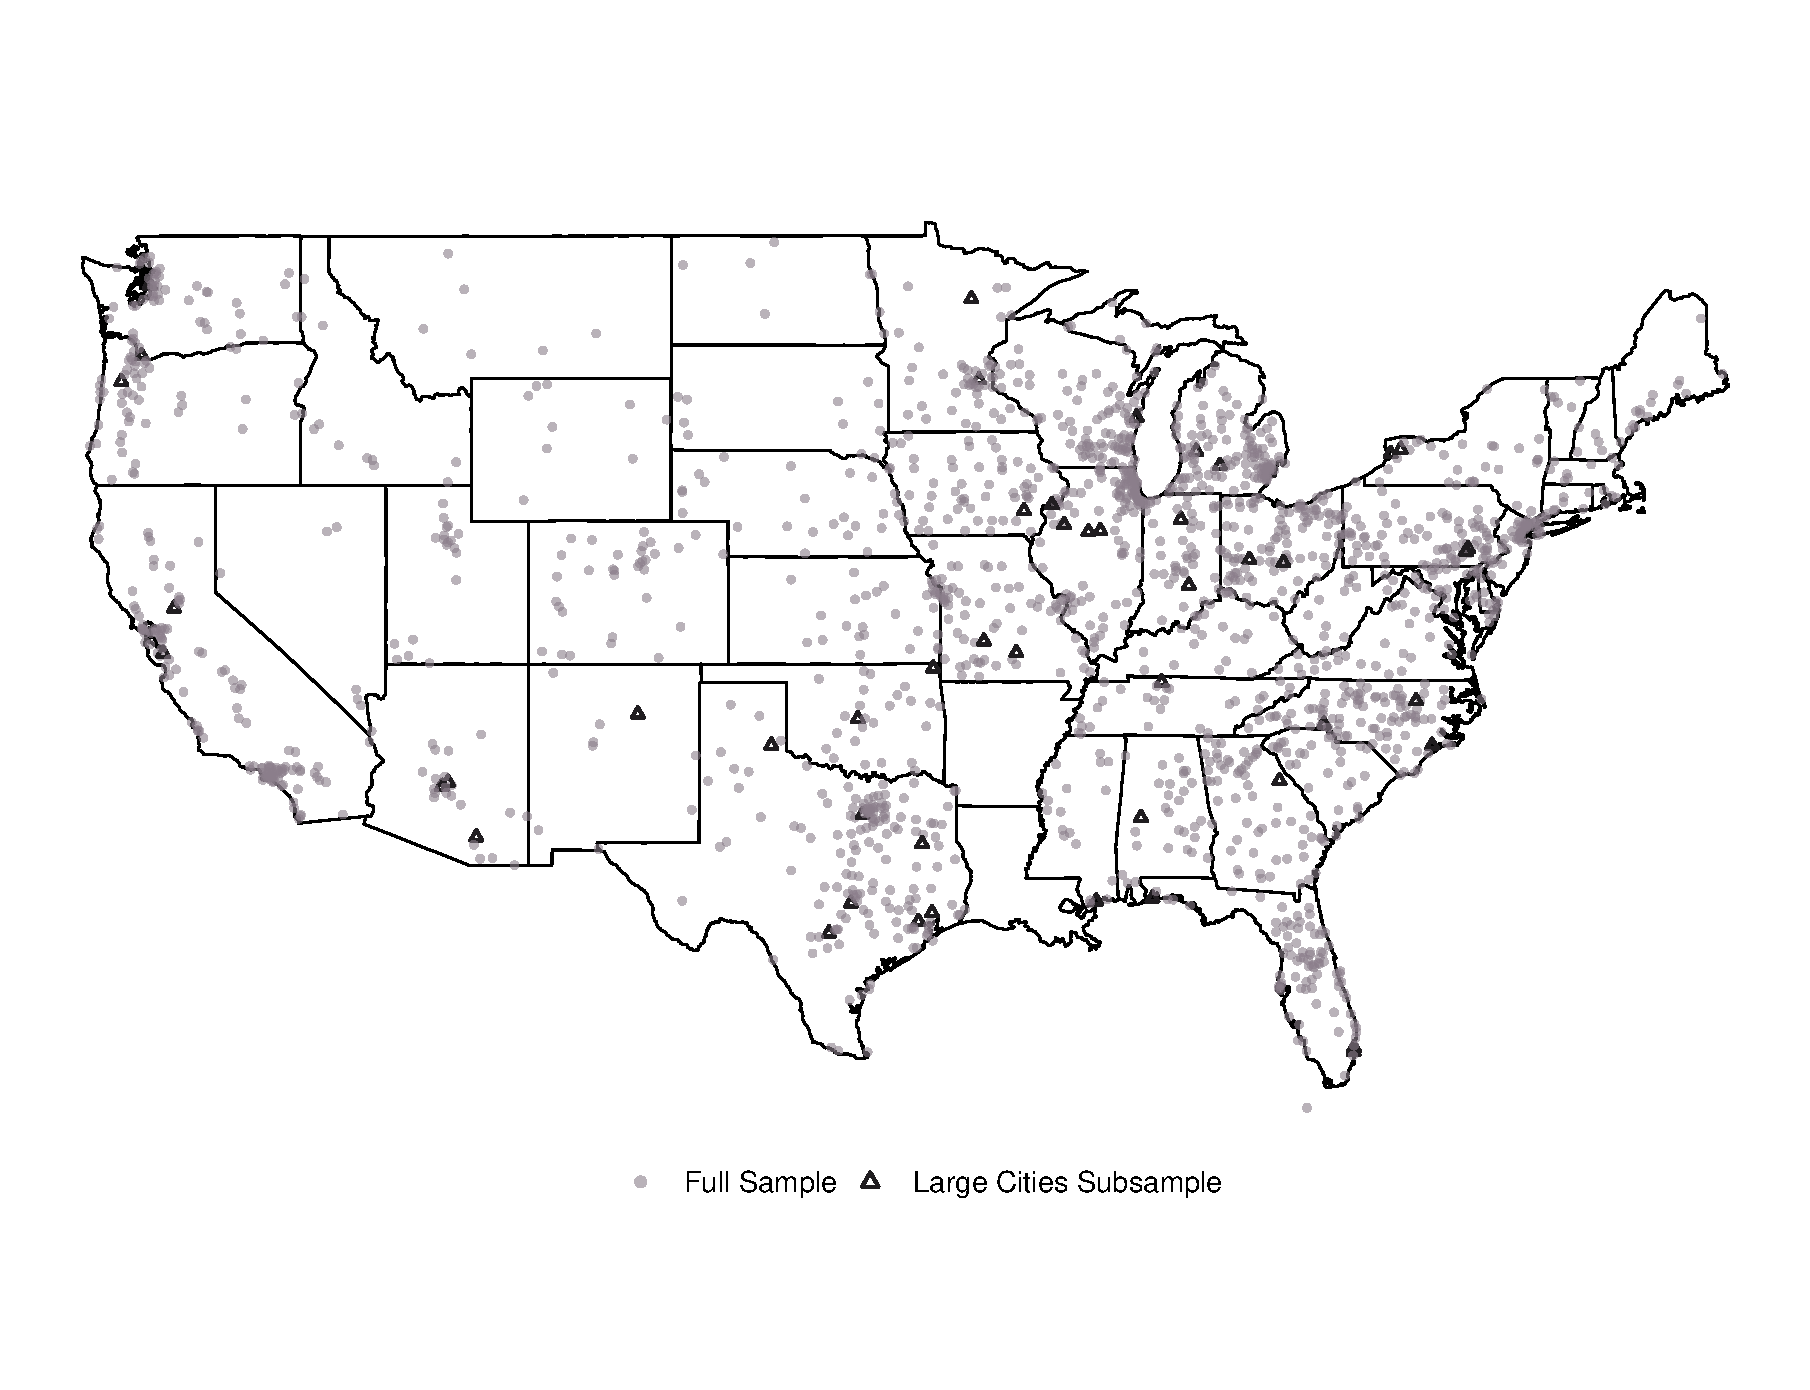
\includegraphics[width=\linewidth]{Figures/SampleMap.pdf}
    }
    \caption[Included Cities Map]{Cities included within my full sample (2,216) and large cities subsample (72).}
    \label{fig:SampleMap}
\end{figure}
 

As cities grow, the size and scope of both their internal governments and local services fundamentally change \citep{oliverDemocracySuburbia2001,oliverLocalElectionsPolitics2012}. Individuals within sparse rural areas such as Carlinville, IL (4,000) may interact inherently differently with local government and their services than individuals from a large urban center such as Chicago, IL (2.75 million) \citep{mooreMotivationsMobilizationComparing2022,debenedictis-kessnerStrategicGovernmentCommunication2022,lassenJurisdictionSizeLocal2011}. Moreover, from the large body of work examining the urban/rural divide within the U.S., an individual's partisan identity may also vary across these local contexts \citep{gimpelUrbanruralDivideResidential2023,nemereverContentiousFederalismSheriffs2021,scalaPoliticalPolarizationRuralUrban2017}. Thus, my results in the following sections may not map perfectly to these smaller American democracies. However, given that I identify clear trends within my larger sample and nearly 40\% of Americans still reside within similarly large cities, my proceeding analyses should provide valuable insight into mechanisms of local polarization and the relationship between local services and individuals' partisan identities.

\subsection{Reexamining Schools and Police}

For each of the 72 cities in my subset, I collected the reported 2018 violent and property crime rates reported by the city to the UCR program. While these measures help to alleviate concerns associated with county-level estimates, they still suffer from problems associated with using crime rates to gauge police performance. To supplement these rates, I also include the number of employees each city employs within its police department. I standardize these measures to the number of employees per 100,000 citizens to compare across municipalities of varying sizes. While the number of employees is not directly correlated to a city's ability to combat crime, it serves as a proxy for city-level spending on policing. For school performance, I use the identical standardized test scores used in the primary analysis.


 One of the critical problems present in my primary analysis above is that an individual's partisanship is not assigned randomly. One's partisan identity is closely correlated with various other identities influencing access to local services and selective residency. In an effort to combat concerns of endogenous confounding, I employ a procedure of covariate balanced propensity score weighting (CBPSW) as presented in \citet{imaiCovariateBalancingPropensity2014}. To improve matching, I match respondents on each of the previous controls included in the initial analysis in addition to city-specific objective performance measures. Using these weights, I then regress the effect of partisanship on evaluations of both local schools and police using both random state and municipality effects and present the results in \autoref{tab:CBPS}. Due to the variability associated with choosing weights, I opt to bootstrap the standard errors for my estimates. I recalculate the matches and fit the hierarchical model for each bootstrapped sample.


\begin{table}[H] \centering 
  \caption{Large City Analysis Using CBPS Weighting of Partisanship on Local Evaluations} 
  \label{tab:CBPS} 
  \scalebox{0.75}{
\begin{tabular}{@{\extracolsep{5pt}}lcc} 
\\[-1.8ex]\hline 
\hline \\[-1.8ex] 
 & \multicolumn{2}{c}{\textit{Service Evaluation:}} \\ 
\cline{2-3} 
\\[-1.8ex] & School & Police \\ 
\hline \\[-1.8ex] 
 Republican & $-$0.043 & 0.262$^{*}$ \\ 
  & (0.027) & (0.029) \\ 
  & & \\ 
 Constant & 0.240$^{*}$ & 0.345$^{*}$ \\ 
  & (0.063) & (0.042) \\ 
  & & \\ 
\hline \\[-1.8ex] 
Observations & 7,591 & 4,956 \\ 
AIC & 24,304.160 & 14,917.710 \\ 
\hline 
\hline \\[-1.8ex] 
\end{tabular} }
\begin{tablenotes}
    \item {\footnotesize Note: The above table presents the results of a CBPS Weighting with bootstrapped standard errors for my large cities sample. Bootstrapped standard errors are presented in parentheses. $^{*}$p$<$0.05}
\end{tablenotes}
\end{table} 

From the table above, the coefficients surrounding \textit{Republican} are again statistically significant at a $p<0.05$ level for police, while a similar pattern is not seen for schools. Additionally, the effect of partisanship in the case of police appears to be similar to my initial analysis despite the inclusion of additional city-specific measures. I should note, however,  that CBPSW does not completely solve all concerns of endogeneity as the process is still sensitive to large misspecifications of the modeling process. Accounting for all possible confounders associated with one's partisan identity and interaction with local services is nearly impossible for this form of observational study; however, this procedure provides more probable estimates than those generated by traditional forms of regression alone. 

\subsection{An Alternative to Schools}
There may be some concern that schools do not provide an adequate contrast to test my theory of polarization. Given trends following nationwide shutdowns in response to the COVID-19 pandemic, some may argue that schools are far more polarized than I posit earlier in this paper. Luckily, given my focus on larger cities, I can examine another prominent local service: roads. While roads may receive less media or political attention, they are a salient service most individuals interact with to some degree on a daily basis. One objective measure of roads is traffic congestion. Using historic traffic data provided by TomTom, a popular transportation and navigation service, I assigned each city an index measure for their average level of traffic for the year 2018. \textit{Traffic Index} is measured on a 0 to 100 scale and calculated--- through GPS data---by measuring the average additional travel time traffic congestion adds to a standard 30-minute trip within a given city. For ease of calculation and interpretability, I employ a hierarchical linear regression that includes state- and city-level random effects and display my results in the table below.

\begin{table}[H] \centering 
  \caption{Hierarchical Linear Regression of Local Roads  Evaluation on Partisan Identity: Full Results} 
  \label{} 
  \scalebox{0.75}{
\begin{tabular}{@{\extracolsep{5pt}}lc} 
\\[-1.8ex]\hline 
\hline \\[-1.8ex] 
 & \multicolumn{1}{c}{\textit{Service Evaluation:}} \\ 
\cline{2-2} 
\\[-1.8ex] & Roads \\ 
\hline \\[-1.8ex] 
  Republican & 0.030 \\ 
  & (0.026) \\ 
  & \\ 
 Traffic Index & $-$0.003 \\ 
  & (0.003) \\ 
  & \\ 
 Age & $-$0.005$^{*}$ \\ 
  & (0.001) \\ 
  & \\ 
 Gender (M) & 0.020 \\ 
  & (0.022) \\ 
  & \\ 
 Black & $-$0.175$^{*}$ \\ 
  & (0.033) \\ 
  & \\ 
 Income & 0.016$^{*}$ \\ 
  & (0.004) \\ 
  & \\ 
 Constant & $-$0.003 \\ 
  & (0.077) \\ 
  & \\ 
\hline \\[-1.8ex] 
Observations & 6,928 \\ 
State Random Effects & \ding{51} \\ 
Municipality Random Effects & \ding{51} \\
Additional Controls & \ding{51}\\
AIC & 18,191.980 \\ 
\hline 
\hline \\[-1.8ex] 
\end{tabular} }
\begin{tablenotes}
    \item {\footnotesize Note: The above table presents the results of a hierarchical linear regression with random effects. All respondents are nested within municipalities within states. Full regression results can be found within the appendix. Standard errors are presented in parentheses.$^{*}$p$<$0.05}
\end{tablenotes}
\end{table} 

The results from Table 3 above suggest that one's partisan identity does not appear to play a significant role in their evaluations of local roads. However, the average traffic conditions do not significantly affect an individual's evaluations either. This finding could be because individuals use alternative cues, such as pavement conditions, to measure road quality. Alternatively, individuals may not have a conception of the annual performance of roads and instead base their evaluations on road conditions immediately surrounding when the survey was fielded. If this were the case, annual measures of road conditions may be poor objective performance measures for local road quality. Despite this finding, the results surrounding partisanship support my theory of polarized local services. Additionally, these results align with previous work examining road conditions, such as \citet{arceneauxDoesFederalismWeaken2005} and \citet{debenedictis-kessnerHowAttributionInhibits2018}, which find an inconsistent correlation between road and traffic conditions and perceived mayoral performance.

\subsection{Party Position Taking or Elite Valence?}
While the results thus far have supported my claim that for polarized services, individuals' partisan identities bias their evaluations, it remains to be seen as the exact mechanism behind this bias. As mentioned previously in this paper, this bias could be individuals adopting their national party's stance towards a service (i.e., favorability in the case of policing); however, it could also be caused by some form of partisan penalty/reward depending on which party holds political control. To examine this possibility, I borrow from \citet{debenedictis-kessnerAccountabilityLocalEconomy2020} analysis of the effect of mayoral partisanship on municipal spending to record the partisanship of each city's mayor and governor as of 2018 for each city within my large city subsample. I opt to control for both state and local partisan control due to the potentially blurred lines of responsibility for some local goods. While work such as \citet{arceneauxFederalFaceVoting2006} suggests that individuals can make meaningful distinctions between levels of government, they also highlight that this ability depends on an individual's perceived responsibilities of local, state, and federal governments \citep{arceneauxDoesFederalismWeaken2005}. The growing trend of nationalization and politicization may lead individuals to view state and federal governments as increasingly responsible for some local policy areas. For the analysis,  I employ a similar hierarchical regression as before and present the results in \autoref{tab:MayorParty}. 

\begin{table}[H] \centering 
  \caption{Hierarchical Linear Regression of State and Local Co-partisanship on Local Service Evaluations} 
  \label{tab:MayorParty} 
  \scalebox{0.75}{
\begin{tabular}{@{\extracolsep{5pt}}lccc} 
\\[-1.8ex]\hline 
\hline \\[-1.8ex] 
 & \multicolumn{3}{c}{\textit{Service Evaluation:}} \\ 
\cline{2-4} 
\\[-1.8ex] & Police & Roads & Schools \\ 
\hline \\[-1.8ex] 
 Co-partisan Mayor & $-$0.038 & 0.013 & 0.042 \\ 
  & (0.034) & (0.032) & (0.030) \\ 
  & & & \\ 
 Co-partisan Governor & 0.015 & 0.045 & 0.052 \\ 
  & (0.031) & (0.025) & (0.028) \\ 
  & & & \\ 
 Republican & 0.246$^{*}$ & 0.023 & -0.065 \\ 
  & (0.038) & (0.033) & (0.033) \\ 
  & & & \\ 
 Constant & $-$0.057 & $-$0.021 & $-$0.630$^{*}$ \\ 
  & (0.122) & (0.081) & (0.085) \\ 
  & & & \\ 
\hline \\[-1.8ex] 
Observations & 4,750 & 6,846 & 6,908 \\ 
AIC & 12,635.960 & 18,002.590 & 18,953.690 \\ 
State Random Effects & \ding{51} & \ding{51} & \ding{51} \\ 
Municipality Random Effects & \ding{51} & \ding{51} & \ding{51} \\
Objective Measures & \ding{51} & \ding{51} & \ding{51} \\
Additional Controls & \ding{51} & \ding{51} & \ding{51} \\
\hline 
\hline \\[-1.8ex] 
\end{tabular}} 
\begin{tablenotes}
    \item {\footnotesize Note: The above table presents the results of a hierarchical regression for my large cities sample. Respondents are nested within cities and then states. Co-partisanship was determined by whether the respondent shared the party of the acting Governor or Mayor in 2018. Standard errors are presented in the parentheses. $^{*}$p$<$0.05}
\end{tablenotes}
\end{table} 

In the case of all three local services, co-partisanship with either the city's mayor or governor does not significantly affect one's evaluations of local services. Even in the case of police, an individual's evaluations appear to be based far more on their partisan identity rather than their shared partisanship with local officials. While these null results don't necessarily mean shared partisanship does not affect local evaluations, for polarized services, the party's average position matters far more. These null results may be partially explained by the lack of party competition often found within municipal governments \citep{bucchianeriPartyCompetitionCoalitional2020}.



\section{Conclusion}

At the beginning of this article, I argued that individuals' evaluations of municipal services are not necessarily based on the quality of the service or their access to it. Instead, some local services have become polarized, leading to partisan distortions of evaluations in the direction of party preferences. Through an analysis of local police and schools, I provided strong correlational evidence that the polarized discourse surrounding police has led Republicans to evaluate the service more positively than other outpartisans. Additionally, I showed how a similar process is absent in non-polarized cases of local schools and local roads. 

My work adds to our understanding of retrospective evaluations within local politics in several ways. First, it highlights how increased nationalization and partisan sorting may inhibit retrospective voting within a local context. Second, the data used in my analysis departs from the traditionally geographically narrow approaches used to examine local politics and expands my analysis to a national sample. Lastly, it adds to our broader understanding of how polarization shapes electoral accountability. As individuals become increasingly sorted along party lines, my work suggests that retrospective evaluations may become less and less likely at all levels of government.

These findings suggest that partisanship may play a far more prominent role in the realm of local politics than previously conceived. For policymakers, this conclusion is potentially problematic as individuals may begin holding local services accountable for national opinions rather than their objective performance. By doing so, individuals may incentivize policymakers to prioritize polarizing aspects of local services at the potential detriment of the service as a whole. This analysis of local evaluations raises several vital questions surrounding local accountability and responsiveness. Notably, for two of the three examined services, objective measures of the said service failed to impact an individual's evaluation significantly. Future work should examine how individuals construct these perceptions of local services and which measures impact which group's evaluations. Additionally, while I've shown that partisanship may shape local assessments, it remains unclear whether this translates into any policy or electoral change. Examining how local politics' nationalization and potential polarization affect municipal policy-making and spending should be an essential focus of future work.


\chapter{Utilizing Large Language Models To Transform Messy Text-Based Sources In Useful Data}
\label{chap:cahpter3}

Often, political scientists are tasked with transforming text-based primary sources into quantitative datasets. Sources such as newspapers, legal records, and transcripts contain a myriad of valuable information ranging from simple names and counts to specific legislation and institutional features. These data form the backbone of many political datasets, but extracting said data has historically been laborious and time-consuming. Texts are often recorded in formats with human readers in mind, making automated approaches prohibitively challenging to apply to the wide range of styles in which text-based sources may appear. Given this challenge, most researchers extract their desired information by hand or use crowdsourcing to expedite the process \citep{sumnerCrowdsourcingReliableLocal2020,bohannonSocialSciencePennies2011}. However, these solutions come at the cost of time for hand coding and money for crowdsourcing, which is especially problematic if researchers wish to rely on accurate information and require multiple crowdsources to compare results \citep{benoitCrowdsourcedTextAnalysis2016,carlsonPairwiseComparisonFramework2017}. These costs force many researchers to limit their focus to a subset of features and texts that either share commonalities in formats or are simply manageable to transform. By doing so, researchers sacrifice potential substantive coverage and cannot update datasets to reflect changing trends.\footnote{For example, \citet{debenedictis-kessnerMayoralPartisanshipMunicipal2016} highlight this exact problem for the field of local politics.} Moreover, after the information is extracted from these sources, researchers are locked in and can only gather new data (even if it's within the same text-based sources) if they repeat the expensive process.

    To alleviate this problem throughout political science, I propose a human-in-the-loop pipeline that leverages recent advances in Large Language Models (LLMs) to crowdsource and transform text-based sources into quantifiable datasets artificially. At its core, the process involves the iterative construction of instructions and context for a model and then the model's implementation of them to transform text into usable data efficiently. Researchers hand code a selection of their texts and then use it to measure LLM performance and adjust the contextual settings provided to the model. The pipeline relies on the foundational nature of LLMs \citep{bommasaniOpportunitiesRisksFoundation2022}, which allows them to complete various tasks outside \citep{brownLanguageModelsAre2020,radfordLanguageModelsAre2019} and within political science \citep{argyleOutOneMany2023,haffnerIntroducingInterpretableDeep2023,laurerLessAnnotatingMore2023,wangFinetuningLargeLanguage2023,ornsteinHowTrainYour}. Importantly, LLMs are far faster than human coders and can cost an order of magnitude less. However, LLMs are imperfect and can suffer inaccuracy or hallucinations wherein the model creates data that is not present within the text \citep{bommasaniOpportunitiesRisksFoundation2022,benderDangersStochasticParrots2021,karpinskaLargeLanguageModels2023}. These complications can make it difficult for researchers to gauge whether these models produce accurate data or whether false or unreliable results contaminate the final dataset. The iterative nature of the pipeline works to address this concern by providing researchers with a validation of the model's performance and allows them to find and understand potential points of friction \citep{grimmerTextDataPromise2013}. By leveraging both the researcher's judgment in the data quality process and the speed and adaptability of LLMS, researchers can more efficiently transform a greater variety of text-based sources into valuable datasets.

    I demonstrate the pipeline with two examples from local and judicial politics. Both examples involve extracting meaningful information from text-based government and legal documents, a task common throughout numerous fields of political science. For each case, I hand-coded a small sample of documents and used them to train a model to transform the corpus into a quantitative dataset. I then compare the model's performance with expert coders assigned the same task. Overall, I find that LLMs produce results comparable to professional coders and, in a process, far more technically accessible than other machine learning solutions. Crucially, after a model was iteratively tuned to the task, LLMs could accomplish the coding tasks in mere hours rather than the days or weeks required to transform the data by hand.

    In summary, this pipeline has the potential to significantly enhance the process of transforming and coding text-based sources. While it may not entirely eliminate the need for manual coding, it can considerably reduce the manual labor required to produce high-quality data. Additionally, it provides researchers with an adaptable framework for text transformation. By incorporating additional manually coded data, LLMs can quickly capture data that researchers may have missed or overlooked during the initial coding process. Beyond transforming datasets, this process contributes to the broader push for transparency in political science research by allowing researchers to clarify their data processing methods, facilitating replication and expansion of their work \citep{gaikwadTransparencyTextBasedSources2023}.

    The paper proceeds as follows. First, I expand on the difficulties of transforming text into data and why automating it has historically been challenging. Second, I provide additional information regarding LLMs, including what they are, how they are trained, and why they are perfect for this specific application. Third, I outline my pipeline, including best practices and example implementations. Fourth, I demonstrate the model with two unique case studies and conclude with potential applications and pitfalls of using LLMs as artificial crowd coders.

    \section{Why is Transforming Text-Based Sources Difficult?}
    
    Transforming text-based sources into quantifiable datasets is a deceptively simple problem. Our desired data is often contained directly within texts, and we only need to locate it, extract it, and format it into our final dataset. However, this process is often more complex than we might initially think. For example, if we want to extract all interest groups who sign an amicus curiae brief to the Supreme Court, much like \citet{Box-Steffensmeier:2012d}. We need to locate the section of the brief that lists the interest groups that signed the brief, which may vary on a brief-by-brief basis. Next, we need only to extract the interest who signed the brief, not their legal counsel or other mentioned groups. Finally, we must store those interest group names in our desired data format. For researchers who either hand-code the data or utilize crowd-sourcing, this process is manageable as they can easily see the organizations in the appropriate section of the brief and extract their names. Ideally, each brief would then be coded multiple times to ensure coders accurately extracted all interest groups. However, this process can be tedious, time-consuming, and potentially expensive, especially as the number of briefs grows.

    In most cases, researchers have limited resources and may only code each document once, often by a singular coder, thus forgoing many benefits of crowd-sourcing data \citep{benoitCrowdsourcedTextAnalysis2016}. Hand coding and crowd-sourcing text-based sources have been the backbone of political science research. Still, their associated costs mean researchers are often limited in the amount and variety of data they reasonably process. Alternatively, researchers could turn to computer-assisted methods to transform text-based sources, but these methods bring additional challenges.

    Transforming text-based sources into quantifiable data through computer-assisted means is far from a novel problem. Within political science alone, approaches such as regular expressions, named entity recognition (NER) \citep{kerkvliet-etal-2020-mentions,jalalPerformanceComparisonCrowdworkers2020}, and optical character recognition (OCR) \citep{permaloffOpticalCharacterRecognition1992a} have long been utilized to identify and extract meaningful information from text, including names, dates, locations, and amounts from text. In theory, each of these methods can efficiently transform many text-based sources present throughout political science but often require extensive fine-tuning and adjustments to transform data correctly. While researchers could lessen these burdens by utilizing out-of-the-box models or fine-tuning pre-trained models to extract their desired information or fine-tuned pre-trained models \citep{laurerLessAnnotatingMore2023}, producing an automated process that works for a large variety of texts can be exceedingly challenging.

    The core problem with transforming text-based sources is that the information we desire may take a myriad of forms, making it difficult to process automatically. While many individual text-based sources may follow consistent formatting, when researchers look across units (i.e., across different sources of texts), formats can vary wildly. This heterogeneity in how information is stored is not limited to between-unit examinations but is also present within units. Recording practices may change over the years as maintainers of these records adopt new services or standards.\footnote{A common example of this is with municipal records, which can vary depending on who is the municipal clerk.} This problem is especially present when researchers examine longitudinal sets of texts where reporting practices may change over time, even if the core information remains present throughout. \autoref{fig:election} displays an illustrative example of formatting discrepancies within the precinct-level municipal election returns from the city of St. Louis and the county of St. Louis. Both returns record the same electoral information regarding the contest and vote breakdown but in starkly different formats.\footnote{Precinct level electoral returns, in particular, have proven exceptionally difficult to gather and quantify. Even recent groundbreaking efforts such as \citet{debenedictis-kessnerAmericanLocalGovernment2023}'s local election database or previous advances such as \citet{marschallStudyLocalElections2011}'s LEAP only cover a sample of all electoral races and results in the United States.} Each format could require a novel automated method or special modification to transform accurately. Even if automated methods successfully transform and extract a researcher's desired data, they may fail to consider the context of the information.


    \begin{figure}[H]
        \centering
        \begin{subfigure}{0.65\textwidth} % Adjust the width as needed
            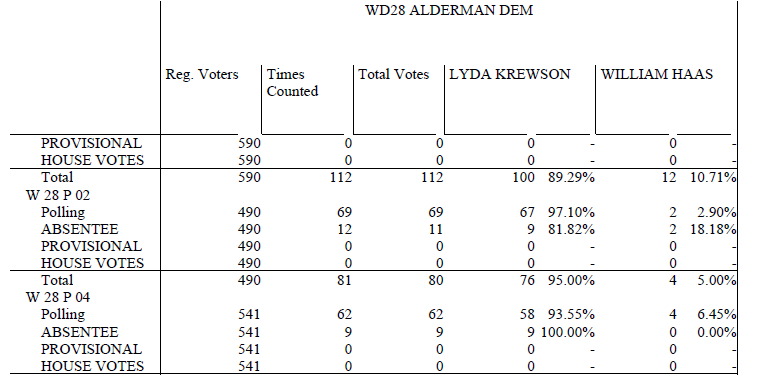
\includegraphics[width=\linewidth]{Figures/CityElection.png} % Replace "image1" with your image file name
            \caption{St. Louis City}
        \end{subfigure}
        
        \vspace{15pt} % Add some vertical space between the subfigures
        
        \begin{subfigure}{0.99\textwidth} % Adjust the width as needed
            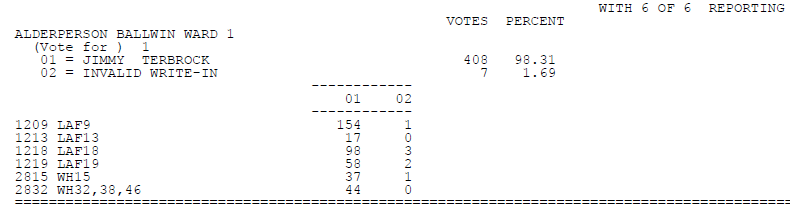
\includegraphics[width=\linewidth]{Figures/CountyElection.png} % Replace "image2" with your image file name
            \caption{St. Louis County}
        \end{subfigure}
        
        \caption[Precinct Level Election Results Example]{Snapshots of official precinct level results from the 2015 General Municipal elections. Both examples cover separate aldermanic races occuring that year.}
        \label{fig:election}
    \end{figure}


    Often, texts include a plethora of information that may not be relevant to our research question. We may only be interested in information when it pertains to specific concepts or is related to particular entities. For example, we may be interested in the kinds of citizens who participate in public town hall meetings and the types of comments they make. A possible text-based source to examine this question would be transcripts of the meetings from the Local View dataset \citep{barariLocalViewDatabasePublic2023}. We would want to extract each commenter's name and comment for each meeting. However, citizens are not the only individuals to participate in these meetings, and we would want to filter out public officials who may be leading the discussion. Citizens may also talk in groups or multiple times throughout a meeting, and we would like to associate each citizen with all the comments they make. Human coders could, albeit tediously, accomplish this task as they could understand both the context as to whether an individual was a citizen and whether each transcribed portion of the meeting belonged to a specific individual. In the case of automated approaches, this task can quickly grow in complexity, as even if automated approaches can identify comments and commenters, researchers would be forced to devise a schema to filter out unwanted participates and to associate comments with individual commenters.\footnote{I should note that recent advances NER and OCR based approaches can successfully associate entities within texts, but they would likely still require some amount of training and fine-tuning to function successfully \citep{kimOCRfreeDocumentUnderstanding2022}} The need for context around information need not even be so complex. It can be as simple as only wanting specific dates or monetary values from texts, both of which might require some level of contextual awareness to identify correctly.

    Transforming text-based sources is not an impossible task, but hand coding can be costly in terms of time and resources, and automated approaches often require significant labor to get up and running and are inflexible to new cases. There is a need for an approach that combines the adaptability of hand coding with efficient automated approaches. I propose that we can employ LLM to meet this need and improve the number and variety of text-based sources we transform into usable datasets.



    \section{What are LLMs and How Can They Help?}
    The term LLM refers to a family of deep learning models built upon a \textit{transformer} framework \citep{vaswaniAttentionAllYou2017}. Hallmarks of these models include immense training sets comprised of a variety of text sources ranging from web content, code, or even classical literature and billions (or, at the time of writing, trillions) of individual parameters, which allow these models to understand the human language on a previously unprecedented level \citep{adiwardanaHumanlikeOpenDomainChatbot2020,brownLanguageModelsAre2020,radfordLanguageModelsAre2019}. While there currently exists a plethora of LLMs, each with its unique size, scope, and intended purpose, in the interest of this paper I will focus primarily on the application of large generative language models such as OpenAI’s GPT-3 \citep{brownLanguageModelsAre2020}, Google’s Lambda \citep{thoppilanLaMDALanguageModels2022} or the open-sourced LLama \citep{touvronLLaMAOpenEfficient2023} and BLOOM \citep{scaoBLOOM176BParameterOpenAccess2023} models. At the most basic level, these larger models are trained to predict words and phrases in response to some initial prompt or context. For example, when presented with the question “What color is the sky?” the model may respond with “Blue” as this is the most probable response to the initial question.\footnote{This is a general overview of how these models function. Models include a variety of other features, such as context windows or temperature. Models can also be trained with additional Reinforcement Learning with Human Feedback (RLHF), which influence a model's ability to respond to specific contexts \citep{ouyangTrainingLanguageModels2022}.}

    Despite the seeming simplicity of this design, these models have shown a remarkable ability to perform emergent capabilities ranging from replicating common natural language processing tasks (e.g., sentiment analysis, classification, and topic modeling) \citep{brownLanguageModelsAre2020,ornsteinHowTrainYour}, to performing information retrieval tasks \citep{zhouFrequencybasedDistortionsContextualized2021}, or even generating synthetic human responses to survey questions \citep{argyleOutOneMany2023}. LLMs perform these emergent tasks by changing the core tasks into a series of next-word prediction tasks. Models are presented with some form of prompt or initial context and then tasked with generating a response in accordance with some set of rules. For example, a researcher interested in obtaining the sentiment of tweets might ask the model whether a tweet is positive, negative, or neutral in tone and then provide the tweet's text. The model would then give the most probable response from that selection of options. To further improve a model's performance, researchers can provide examples of desired responses, commonly referred to as one or few-shot learning examples \citep{lazaridouInternetaugmentedLanguageModels2022}.

    I propose that we can turn the transformation of text-based sources into a next-word prediction task and then have these large-scale models complete them as synthetic coders. By providing these models with our text-based source and a prompt detailing how we want it processed, we can leverage the advanced capabilities of these models to transform texts in an adaptable and efficient fashion. Specifically, I suggest we provide these models with instructions—much akin to instructions for human coders—regarding the type of information we want from texts and then have the model identify, extract, and format said information into quantifiable datasets. These models' ability to understand the contextual features of text allows them to overcome many of the hurdles associated with prior automated approaches and produce near-human-quality coding responses. However, these models should not synthetically code all text-based sources without validation.

    While impressive, LLMs have several limitations that may negatively affect their ability to code text-based sources. First, these models are trained on a large variety of human-generated data and, as such, can express many of the same biases and stereotypes present within these data \citep{gargWordEmbeddingsQuantify2018,caliskanSemanticsDerivedAutomatically2017,benderDangersStochasticParrots2021,zhouFrequencybasedDistortionsContextualized2021}. These reflected biases may be especially concerning for political science research as models may systematically misidentify information pertaining to marginalized groups. For example, a model tasked with identifying government officials with a piece of text may inappropriately identify (or misidentify) individuals along the lines of gender or race. Second, these models can produce noisy results or hallucinate data not initially present within the original text \citep{linTruthfulQAMeasuringHow2022}. In either case, the incorrect data may be difficult to spot and contaminate the final dataset in unseen ways. Given these potential problems with LLMs, researchers must have some way to validate the output of these models \citep{grimmerTextDataPromise2013,knoxTestingCausalTheories2022}. Therefore, in the following section, I propose a human-in-the-loop process in which researchers iteratively design the context for these models and then validate their performance on a subset of their data to identify—and ideally minimize—instances of error and bias.

    \section{The Proposed Pipeline}


    Following many of the principles from recent advances in adaptive machine learning \citep{enamoradoUsingProbabilisticModel2019,wiedemannProportionalClassificationRevisited2019,millerActiveLearningApproaches2020}, the framework relies on leveraging LLMs efficiency to process some text-based sources and then utilizing humans to correct and guide these models to the correct answer \citep{mozerMatchingTextData2019}. While most applications of adaptive machine learning rely on the models to iteratively update based on human input, this process follows an alternative approach. Much like a researcher would update instructions for human coders, the researcher updates parameters and inputs in response to the model's performance. The process consists of hand coding a subset of data and then using that data to improve the prompt and context sent to the LLM iteratively. Once the LLM achieves a researcher's desired level of accuracy, it is used to transform the remaining data. \autoref{fig:workflow} provides an overview of each of the steps within the workflow. Notably, the process overall is agnostic to the exact LLM utilized, but as detailed below, the model's characteristics may substantially affect a researcher's choices throughout the process.

    \begin{figure}[H]
        \centering
        \begin{tikzpicture}
            % Define nodes
        \node[draw,
        rounded rectangle,
        minimum width=2.5cm,
        minimum height=1cm] (block1) {Preprocess Text};
     
     
        \node[draw,
        rectangle,
        below=of block1,
        minimum width=2.5cm,
        minimum height=1cm] (block2) { Subset and hand code training set};
     

        \node[draw,
        rectangle,
        below =of block2,
        minimum width=2.5cm,
        minimum height=1cm] (block3) {Create prompt with instructions};
    
        \node[draw,
        rectangle,
        below =of block3,
        minimum width=2.5cm,
        minimum height=1cm] (block4) {Choose text context};

        
        \node[draw,
        rectangle,
        below =of block4,
        minimum width=2.5cm,
        minimum height=1cm] (block5) {Process training data with LLM};

        \node[draw,
        rectangle,
        below =of block5,
        minimum width=2.5cm,
        minimum height=1cm] (block6) {Evaluate LLM performance};
    
        \node[draw,
        rectangle,
        below=of block6,
        minimum width=2.5cm,
        minimum height=1cm] (block7) {Process unlabeled data};

        \node[draw,
        rectangle,
        right =of block4,
        minimum width=2.5cm,
        minimum height=1cm] (block8) {Repeat until model achieves set error rate};
    

        \draw [arrow] (block1) -- (block2);
        \draw [arrow] (block2) -- (block3);
        \draw [arrow] (block3) -- (block4);
        \draw [arrow] (block4) -- (block5);
        \draw [arrow] (block5) -- (block6);
        \draw [arrow] (block6) -- (block7);
        \draw [arrow] (block6) -| (block8);
        \draw [arrow] (block8) |- (block3);
        

        \end{tikzpicture}
        \caption[Framework for using Large Lanaguage Models to transform text-based sources.]{Framework for using Large Lanaguage Models to transform text-based sources.}
        \label{fig:workflow}
    \end{figure}

    \subsection{Preparing Text-Based Sources}
    The first step of the workflow is to preprocess the text into some machine-readable format. Like most text-as-data approaches, how we preprocess the text can significantly affect our final results \citep{grimmer2022text,wilkersonLargeScaleComputerizedText2017}. However, unlike most preprocessing for NLP, we want to be careful not to remove too much from the texts. We want our text to maintain its rough format and maintain any important contextual features surrounding our desired data. For texts that require some form of OCR, as is the case with many legal and government documents, we need to be aware that the quality of the transformed text may affect their data of interest. Poorly converted data can inhibit even LLM's performance by potentially obfuscating our desired data within the text \citep{vanstrienAssessingImpactOCR2020}. 

    Next, we must divide some of our texts into a training set. This training set aims to validate the LLM's performance, so it should represent a wide variety of texts within our corpus. If we draw on texts from multiple sources, the training set should include examples from each source. Similarly, if we rely on text spanning numerous years, the training set should consist of some texts from each period present within the corpus. For each text within this set, we must manually code the text into our desired data format. This set will be used as the golden standard to compare the performance of the LLM. There is no hard-set rule regarding the size of a training set, although most conventual splits for machine learning rely on splitting at least 20 percent of the sample into a training set. Notably, larger training set sizes will allow researchers to better check the LLM's performance at the cost of additional hand coding.\footnote{Several notable advances have been made in optimizing one's choice in training sets \citep{kaufmanSelectingMoreInformative2024}. Although it is not clear whether they could be applied in this context.} After successfully dividing our corpus, we can begin constructing the prompt for our LLM.

    \subsection{Selecting a Prompt and Context}
    Much like human coders, models require some form of text-based instructions to generate responses. This prompt details the instructions for the model and will be our primary point of iteration and revision throughout the workflow. While the exact wording of our prompt will vary depending on our text and desired data, the prompt should include three key components. First, we should specify the information we wish to extract from the text. We should be as specific as possible in this stage, as more detailed descriptions tend to lead to higher-quality outputs from the model. Second, is the format we want the model to return our data in.\footnote{Given most LLMs are trained on a large body of code, we may opt to have the model return the results in a data format from our preferred coding language (e.g., a data frame within R, or a dictionary within Python).} Beyond making it easier to process the data output from the model, having a consistent output can make it easier for us to detect errors. In addition to these formatting instructions, we should provide instructions on what the model should do when the desired data is absent from a text. By doing so, we can reduce unexpected responses from the model and provide a clear null case during the validation step. Finally, a one or few-shot learning example of the desired output data. For example, again, in the case of obtaining sentiment from a tweet, we would want to include examples of tweets and their respective coding. These training examples can significantly improve an LLM's performance and help the model produce consistent results \citep{brownLanguageModelsAre2020}. If including a full training example is not feasible due to the type of desired data or length of the text, we can include an example output to obtain a similar effect on model performance and consistency.\footnote{I show an example of this practice within both case studies later in this article.}

    Our last choice in the workflow is the context of the text to share with the model. Specifically, how much of the text-based source should be included following the prompt? All LLMs have a maximum sequence window. These windows are primarily a factor of the model's number of parameters and effectively dictate how much text the model can intake and output at a time. Most models have context windows between 2048 and 8000 tokens.\footnote{Tokens are sequences of characters representing meaningful units of text. Usually, tokens consist of one or more words, but different models utilize different tokenizers to preprocess text.} Given these limits, we must be careful regarding how we present our text to the model. For smaller texts, we can freely include the entirety of the text following the prompt. However, for larger texts, we may need to split the text into sections and have the model process each section. If we break our texts, we should consider how the splits may affect our desired information. We may inadvertently split a section of desired information and effectively cut it out of the text we provide the model. Beyond context windows, we may want to give the model specific sections of text to limit the chances of false positives or cut down on the total text sent to the model. For example, if we only care about information present at the beginning of a document, it would be faster and potentially safer only to provide said section to model rather than the entirety of the text. However, if our desired information could occur throughout a text, we would need to give the entirety of the text to the model.

    Before we process our training data, we may need to decide on a few additional model parameters. These parameters vary between models but often include a maximum response length, a starting seed, or model temperature. Of these parameters, a model's temperature is the most likely to affect the model's capacity to process text-based sources. Conceptually, a model's temperature dictates the diversity in its responses. Often, individuals will equate this parameter to a model's practical creativity. In the context of next word prediction, a model may not choose the most probable word in every case and instead choose an alternative, less likely word or phrase. Given this workflow aims to produce consistent results from text-based sources, we will want to use lower model temperatures.

\subsection{Processing, Iterating, and Validating}
    With our prompt, context, and ancillary parameters decided, we can finally ask the LLM to transform our training data. Most LLMs can be sent data directly through an API.\footnote{Popular models often also include an official or popular open-sourced package that facilitates interacting with their APIs in the most popular coding languages (see the ```text2data``` package from \citet{ornsteinHowTrainYour} as an example.)} For each text within our training set, we will send the model our specific prompt and context and then store its response. Since it can be difficult to anticipate whether our early prompts will be effective, we may want to start with a small portion of our training set and slowly incorporate more of our data as we finetune the model.

    After the model processes our training set, we will evaluate its performance using standard accuarcy and calibration metrics . While we will need the model's overall performance to report our uncertainty later, we want to focus on instances in which the model failed to transform text or mislabeled data for the initial iterative process. Were there certain types of text the model failed to process? Does the model include irrelevant data in its response? Did the model show any obvious signs of bias in the data that it correctly or incorrectly identified? Common corrections we may make in response to these questions are increasing the text sent to the model, changing a prompt to be more specific, changing the learning examples, specifying additional cases to exclude from the output, or breaking up transform into separate steps.\footnote{If we are interested in many pieces of information, creating a different prompt for each piece may be more effective.} After correcting our prompt and context, we can repeat our workflow until the model's output is sufficiently similar to our hand-coded data. Like any machine learning approach, LLMs will likely never perfectly correspond to our training data. However, as I highlight in later case studies, obtaining accuracy metrics between 80\% and 95\% is not unreasonable. If we desire to push the model's performance beyond these limits, we may risk effectively "overfitting" to our training set. This "overfitting" can be problematic if our set is not representative of our larger corpus or if we want to transform a new data set.\footnote{To alleviate overfitting concerns, we may wish to hold out a portion of the training set as a validation set for our final model parameters.}  

    Once our model reaches our desired level of accuracy, we can send our unlabeled text to the model. If any errors occur in this process, we may want to adjust our training set to incorporate problematic texts and reiterate through the workflow. After we process all unlabeled texts, we should record our chosen LLM, last prompt, context, and model accuracy and present them clearly within our final results.


    \section{Applications and Validation}

    In the following two applications, I demonstrate how LLMs can efficiently and accurately transform text-based sources into high-quality data. For both applications, I use OpenAI's GPT 3.5-turbo-1106 to identify, extract, and format meaningful information from text-based records across two starkly different areas of political science. I validate the model's performance with a comparison to its predicted performance from the iterative workflow and human-coded data. Examples of each text-based source and how they were processed can be found in Section C.1 of the Appendix.

    \subsection{Extracting Commenters From Local Meeting Minutes}
    Understanding who and how individuals participate in local governmental meetings has become a key area of study for urban politics \citep{einsteinWhoParticipatesLocal2019,einsteinStillMutedLimited2022,yoderDoesPropertyOwnership2020,nuamahCostParticipatingPoor2021,collinsDoesMeetingStyle2021}. Much of this research relies on datasets of political participation constructed directly from publicly available meeting minutes. In many cases, these minutes record the names, comments, and, at times, addresses of those who participate in public meetings. However, extracting this fruitful data takes work. Meeting minutes, while by law include similar information, such as the names of public officials, votes on local policies, and public commenters, they do not follow similar formats.

    The laws mandating meeting minutes frequently lack specificity, and it is up to the local government to determine the style and level of detail in these recorded minutes \citep{oconnorAssemblyRequiredApplication2004}. As a result, meeting minutes can vary substantially in detail and style between any two local governments.\footnote{Section C.1 within the Appendix provides a select sample of minutes from two similar sized cities within the St. Louis region.} Formatting within governments can even change as new governmental clerks are appointed or the government adopts new strategies, formats, or technologies. These limitations make constructing a diverse and longitude dataset of meeting participation an extremely time-intensive task. As a compromise, research within this area often focuses only on a handful of similar local governments \citep[e.g.,][]{yoderDoesPropertyOwnership2020,einsteinWhoParticipatesLocal2019} or infers participation based on national survey responses \citep{nuamahCloseHomePlaceBased2021}. These compromises, however, come at the cost of potentially noisy estimates and limited variation in the types of local governments examined.

    A demand exists within the field to alleviate the burden of processing these minutes, and LLMs could effectively address this need. To demonstrate how LLMs can be applied to this problem, I apply the workflow above to select school board meeting minutes from the St. Louis region. The dataset consists of all the general meeting minutes from 2018 to 2022 for 16 school boards. The data includes 667 separate meetings ranging immensely in style and detail. This sample should provide a wide variety of meeting minutes between local governments and a perfect test of the capabilities of LLMs.

    I start by hand coding each meeting's minutes and extracting the commenters, addresses, and comments for each meeting. In reality, most researchers will only label a small sample of the data, so to mimic that, I randomly select ten meetings from each government to represent my initial training set of 160 meetings. Next, I construct an initial prompt and display the final prompt in  \autoref{fig:meetingprompt}. Given that public comments can occur at any place within a meeting, I feed the model the entirety of the meeting text. For longer meetings, I split the meetings into 3,000 token chunks. I set the model's temperature to 0 and then feed in each meeting with the associated prompt. To evaluate the model, I examine whether the model obtained the full names, addresses, and comments of each commenter within my training set of meetings.\footnote{In the case of the comment's text, I only examined whether the model returned a comment and not necessarily whether the comment's text matched perfectly.} After approximately four iterations of adjusting the prompt, with the primary changes being additional specificity and modifications to the example outputs, the model displayed a precision of 0.934, recall of 0.984, and F1 of 0.957 for the training set. Given these promising estimates, I fed the remaining meeting through the model and evaluated its performance on the entire dataset.

    \begin{figure}[H]
        \centering
        \begin{lstlisting}[language=python,  label={fig:meetingtext}]
        In the following text of recorded public meeting minutes
        can you identify all of the commenters who spoke during 
        the public comment period(s), all of their addresses if 
        available, and all of their complete comments. 
        Return them in a JSON format. Please do not include public
        officials and use NA for any missing information.
        
        Example Output: 
        
         {
          "Name":["Shawn Spencer"],
          "Address":["5005 North Fraser Way"],
          "Comment":["Concerns about recent crime in the community"]
          }
        
        If no one commented please return: 
        
         {
          "Name":["No Commenters"],
          "Address":[""],
          "Comment":[""]
          }
        
        Meeting Text:
        [MEETING MINUTE TEXT]
        
        \end{lstlisting}
        \caption[Prompt to Extract Commenters from Public Meeting Text Using GPT-3]{Prompt to extract commenters from public meeting text using GPT-3}
        \label{fig:meetingprompt}
    \end{figure}

    Overall, the model could accurately extract almost all commenters from the meeting minutes dataset with an average precision score of 0.935. Incredibly, the model exhibited a low false positive rate with an average recall of 0.977. To contextualize these findings, an untrained BERT NER model only achieved a precision of 0.780 and recall of 0.850, requiring extensively more coding and filtering of results.\footnote{More details on the NER application can be found within the Appendix.}  While the LLM successfully parsed most meeting minutes, it failed in a few select cases. The LLM tended to code meetings inaccurately, in which school boards only included the number of total commenters without any form of identifying information. If we would be interested in the count in addition to the commenter's details, we would need to adjust the prompt accordingly or construct a separate one. Another area in which the model struggled was when individuals made detailed and lengthy comments. In these cases, the model would occasionally truncate the comment down. Adjusting the context of the text remedied this problem, but not completely.

    In terms of time to code, the model took approximately 3 hours to fully parse all the meeting minutes at a cost of roughly \$0.01 per meeting. Including the training, the model costs \$8.28 to process the dataset. In comparison, human coding the dataset required an estimated 15 hours to parse the meeting minutes. Beyond being faster and less costly, utilizing an LLM could allow us to parse meetings multiple times for other forms of information, such as the meeting format, the names of public officials, and other critical pieces of information, all only requiring us to hand code a small sample of the entire data.

    
    \subsection{Identifying Interest Groups in Amicus Curiae Briefs}
    Amicus briefs are a valuable tool to estimate interest group's political participation before the Supreme Court. Beyond simple participation, they can reveal underlying political networks \citep{Box-Steffensmeier:2015b}, track  groups' political influence \citep{box-steffensmeierQualityQuantityAmici2013}, and  provide measures of group ideology \citep{abi-hassanIdeologiesOrganizedInterests2023}. To utilize these records, previous researchers hired coders to go brief by brief and extract the names of interest groups and the legal direction of the brief in a time-intensive process. As highlighted previously in this article, the core difficulty with extracting this valuable information from these documents is that organizational names can come in various formats and can vary in their exact placement at the beginning or end of a brief. Identifying the legal direction of a brief is more straightforward as most briefs explicitly state the party they support; however, in a few cases, briefs may report support or opposition of a lower court decision rather than a case's litigants. The combination of varying formats and locations can make correctly identifying either the signers or legal direction difficult, even for human coders. Expediting the processing of these briefs could bring numerous benefits, from easing the maintenance of existing datasets, expanding the coverage of included briefs, or even examining other novel information within the brief's text. LLMs could be applied to these documents to achieve high-quality results at a fraction of the cost and time.

    To demonstrate this application, I utilize the amicus curiae database from \citet{Box-Steffensmeier:2012d}. I focus on all briefs sent to the Court in 2014. This selection narrows the universe of briefs to process but still provides a diverse sample of 190 individual briefs.\footnote{The Court received 351 total briefs in 2014, but only 190 were publicly available and hand-coded at the time of writing.} Subsetting 40 briefs as my training set, I construct the initial prompt and set my initial context as the first and last five pages of each brief. \autoref{fig:briefText} displays the final prompt used to process the text. In each iteration, I evaluate whether the model correctly identified all signers and separately whether it correctly identified the direction of the brief. Given names may vary slightly between the handing coding and the original text of the brief, I allow for some difference between the two sets of names by utilizing a fuzzy string-matching algorithm to detect a match.\footnote{Specifically, I measure the Damerau-Levenshtein distance between the vectors of names and consider a pair a match if their distance is less than five. Given the names were already close, this distance largely accounted for the inclusions/exclusion of words like “the” or “inc.”} After iteratively adjusting the prompt and enlarging the context to the first and last ten pages of each brief, the model identified brief singers with a recall of 0.922 and precision of 0.90 and the legal direction with an accuracy of 0.975.

    \begin{figure}[H]
        \centering
        \begin{lstlisting}[language=python, label={fig:brief-text}]
    In the following amicus curiae brief, which organizations 
    signed the brief and was it for the petitioner, 
    respondent or neither? Please record the organization
    in the form of a Python dictionary. An example 
    of the output is below and then the text to parse. 
    Do not include the law firm who prepared the brief.
             
    Example Outputs: 
    {
      "AMERICA'S ESSENTIAL HOSPITALS" : "Respondent",
      "NATIONAL FEDERATION OF THE BLIND" : "Respondent",
      "TYRELL CORPORATION" : "Respondent"
      }
    
    {
      "EXXON MOBILE" : "Neither",
      "WEYLAND-YUTANI CORPORATION" : "Neither"
     }
    
    Brief Text:
    [BRIEF TEXT]
    \end{lstlisting}
    \caption[Prompt to Extract Signers from Amicus Curiae Briefs Using GPT-3]{Prompt to extract the name of signers from amicus curiae briefs using GPT-3}
    \label{fig:briefText}
    \end{figure}

    When applied to the remaining data, the model displayed a slightly lower average recall of 0.857 and a precision of 0.867.\footnote{Processing the entire dataset cost \$1.18 and took approximately 30 minutes to complete.} While the model did appear to extract the majority of information from briefs correctly, this drop in performance is concerning as, in real applications, it would be unknown to researchers. Upon closer inspection, two primary factors contributed to the performance dip. First, in some cases, the model would incorrectly format responses, leading to all names being considered incorrect. Often, the model would group two or more organizations rather than separate them in the response. Adjusting the prompt to specify this separation or further parsing the model's results would likely solve this issue. Second, the model would sometimes include individuals or agencies in addition to their parent organizations, whereas previous coders only had one or the other. For example, the model may include both the public finance authority for a city and the city itself as signers. Whether this difference is substantively important is unclear but may be addressed by adding further specificity to the prompt. Regarding identifying a brief's legal direction, the model performed similarly to the training set with an accuracy of 0.956. Overall, using an LLM to code briefs seems to be a feasible approach to accelerate the process while maintaining the quality of the final dataset. Nevertheless, the drop in performance between the training and full datasets underscores the potential vulnerability of relying on small training sets to evaluate an LLM's performance.

    
    \section{Discussion}
    Traditionally, the conversion of text-based sources into meaningful datasets has been a laborious and time-consuming task. However, LLMs present a promising solution to this challenge. These models have the potential to combine the efficiency and speed of traditional automated approaches with the flexibility and adaptability of human coders. By iteratively guiding and validating these models, we can create high-quality datasets at a fraction of the cost and time investment. Furthermore, offering details on how we utilized these models, including the prompt, context, and other parameters, provides a unique opportunity to recreate datasets from their original sources. This form of replication, typically avoided due to its high coding costs, can enhance transparency in using text-based sources and facilitate innovation with existing data. Beyond text transformation, LLMs are a promising tool throughout the research process as they assist researchers in effectively handling various data needs, from formatting data to extracting information or even matching across data sources. However, it's essential to acknowledge that despite these promises, my proposed framework and the broader application of LLMs come with their own caveats and challenges.

    Without coding the entirety of the data, it is impossible to guarantee that coding errors and LLMs' potential biases will not permeate into the datasets they help create. It may be fruitful for future work to explore how we could leverage consensus metrics to combine multiple models to minimize the adverse effects of any particular model. Researchers should also recognize that even in the case of the training set for which we have outcomes to compare, it may be challenging to check for all forms of potential bias. For example, in the case of extracting public commenters, researchers may require additional data such as commenter demographics to gauge whether the misclassifies individuals along the lines of gender or race. Such information is often not widely available and can be difficult to match to the original dataset. Overall, the quality of data produced by the model is a product of the diligence and care researchers put into evaluating and validating the model's performance. Researchers should be transparent regarding their implementation of LLMs and aware of potential biases in their final datasets.

    Additionally, while LLMs may alleviate the burden of transforming data, they do not address the initial burden of gathering it in the first place. A researchers’ choice in which sources to include within their dataset can be just as impactful on their study as how they processed their data \citep{gaikwadTransparencyTextBasedSources2023}.  Hopefully by alleviating the pressures of coding each source, LLM can allow researchers to spend more time gathering novel data or better utilize pre-existing collections of data. The latter benefit may be especially promising given recent innovative data collection efforts such as \citep{barariLocalViewDatabasePublic2023}’s collection of meeting transcripts. Each of which holds to potentially to vastly increase our understanding of each of their respective fields. 

    Overall, Large Language Models (LLMs) are a promising tool for future researchers. Like any tool, they should be implemented with transparency and acknowledgment of their potential limitations. If appropriately used, these models offer the potential to drastically increase the accessibility of political science research and expand the coverage and diversity of data used across research domains.


%\chapter{Parts of the Dissertation}
\label{chap:dissertation-parts}

This chapter describes the components of a dissertation.
You may not have to include all components described here, but you must follow the prescribed order for the components you do include.
On \pref{tab:include}, \tref{tab:include} lists the required and optional components in the order that they should appear.
Your manuscript should include three main parts: the front matter, the body, and the back matter.
Each of these parts is described below.

\section{Front Matter}

The front matter includes all material that appears before the beginning of the body of the text.
Number all front matter pages (except the title page and the optional copyright page) with lowercase roman numerals, starting with ii, centered just above the bottom margin.
Each of the following sections should begin on a new page.

\subsection{Title Page}

Format the title page so that it is centered vertically and horizontally on the page with equal amounts of white space from top and bottom margins.
Include a one-inch margin on all sides.
Use a 12-point regular font.
The date on the title page should reflect the month and year the degree is to be officially earned, and should be one of the following months: December, May, or August.
Do \underline{not} include a page number on the title page.
See \hyperref[app:degree-program]{Appendix} for further details.
In most cases your dissertation title should be in ``Title Case'' unless a specific format is required by your discipline.
Be certain to use your own full name (as recorded in \href{https://acadinfo.wustl.edu/}{WebSTAC}).
Following the dissertation chair or co-chair, the faculty should be listed alphabetically by last name.

\begin{table}
	\caption[%
        Required and Optional Thesis Components (NOTE: If you have a multi-lined table label/title,
        then the 2\textsuperscript{nd} and all additional lines should align with the first line, just like this one;
        also, be sure that no words display to the far right hand side where the page numbers for
        your tables display, just as shown in this example.)
    ]{The following items may be included in your dissertation or thesis, in the order in which they are listed.
    Any optional components, if used, \underline{must} be included in the table of contents, unless noted below.}
  \label{tab:include}
  \centering
  \DoubleSpacing

  % Because Times New Roman doesn't have checkmark symbol,
  % Use the checkmark symbol from pifont
  \newcommand{\mycheckmark}{\ding{52}}

  \footnotesize
  \begin{threeparttable}[b]
  \begin{tabular}{@{}ccccc@{}}
  \toprule
    \textbf{Major Part} &
    \makecell[b]{\textbf{Thesis} \\ \textbf{Component}} &
    \textbf{Required} &
    \textbf{Optional} &
    \textbf{Page Numbering} \\
  \midrule

  Front Matter & Title page & \mycheckmark & & counted, not numbered \\
  & Copyright page & & \mycheckmark & neither counted, nor numbered \\
  & Table of Contents & \mycheckmark & & begins on page number \underline{ii} \\
  & List of Figures & & \mycheckmark & [lowercase Roman numerals continue] \\
  & List of Illustrations & & \mycheckmark & [lowercase Roman numerals continue] \\
  & List of Tables & & \mycheckmark & [lowercase Roman numerals continue] \\
  & List of Abbreviations & & \mycheckmark & [lowercase Roman numerals continue] \\
  & Acknowledgments & \mycheckmark & & [lowercase Roman numerals continue] \\
  & Dedication\tnote{*} & & \mycheckmark & [lowercase Roman numerals continue] \\
  & Abstract page & & \mycheckmark & [lowercase Roman numerals continue] \\
  & Preface & & \mycheckmark & [lowercase Roman numerals continue] \\
  Body & Epigraph\tnote{*} & & \mycheckmark & begins on a page numbered \underline{1} \\
  & Chapters & \mycheckmark & & [Arabic numerals begin or continue] \\
  Back Matter & References\tnote{**} & \mycheckmark & & [Arabic numerals continue] \\
  & Appendices & & \mycheckmark & [Arabic numerals continue] \\
  & Curriculum Vitae\tnote{***} & & \mycheckmark & [Arabic numerals continue] \\
  \bottomrule
  \end{tabular}
  \begin{tablenotes}
    \footnotesize
    \item[*] Do not include in the table of contents.
    \item[**] There are two options for the placement of references; they can be listed at the end of each chapter, or at the end of the document.
    \item[***] Do not put your Social Security Number, birthdate, or birthplace on your CV.
  \end{tablenotes}
  \end{threeparttable}
\end{table}

\subsection{Copyright Page}

It is always suggested that upon completion of the text, the student add the copyright symbol © with the year and the student's name on one line, on a page following the title page.
Format your copyright page exactly as it is shown in this template.

\vspace{\onelineskip}
\noindent
\textit{Example:}

\centerline{\textcopyright\ 2022, Paige Turner}
\vspace{\onelineskip}

Once you create a work, it is automatically protected by U.S.\@ copyright law with you as the author.
You do not need to register the copyright with the U.S.\@ Copyright Office, though doing so provides certain advantages.
More information about copyright registration can be found at \href{http://libguides.wustl.edu/copyright/registration}{http://libguides.wustl.edu/copyright/registration}.

\subsection{Table of Contents}

The words ``Table of Contents'' must appear in chapter title style at the top of the page.
It must include the page numbers of all front and back matter elements, unless otherwise specified.
The table of contents must include the page numbers of all chapters and sections of your dissertation.
In addition, it may include the page numbers of all subsections.
Chapter titles may be typed in plain or bold font.
All titles and headings must be followed by a page number.

Make certain that any long titles align nicely with the body of text.
Multi-lined chapter titles or section titles should break at a logical point and align in a manner allowing the titles to be read clearly, without confusion.
Sometimes this will mean forcing a line break at a logical point and relies on your own good judgment.

\subsection{List of Figures}

If one or more figures are used in the document, there must be a list of all figures.
The list should be spaced at 1.15.
Begin each listing on a new line.
Format the list of figures the same way the table of contents is formatted, but put the words ``List of Figures'' in the heading.

\subsection{List of Tables}

If one or more tables are used in the document, there must be a list of all tables.
The list should be spaced at 1.15.
Begin each listing on a new line.
Format the list of tables the same way the table of contents is formatted, but put the words ``List of Tables'' in the heading.

\subsection{List of Abbreviations}

Include a list of abbreviations only if you use abbreviations that are not common in your field.
Arrange the list alphabetically.
Type the words ``List of Abbreviations'' in chapter title style at the top of your list.

\subsection{Acknowledgments}

An acknowledgments section must be included.
Use it to thank those who supported your research through contributions of time, money, or other resources.
Some grants require an acknowledgment.
Type the word ``Acknowledgments'' in chapter title style at the top of your page.
If the acknowledgments fill more than one page, put the heading only on the first page.

\subsection{Dedication}

The dedication page is optional.
If you decide to include a separate dedication page, make it short and center it on the page, both horizontally and vertically.
Do not include it in your table of contents.
See \pref{thesisdedication} for more detailed information.

\subsection{Abstract Page}

An abstract page is optional in the dissertation, but will be required when you submit your manuscript electronically.
Format the abstract page precisely as shown in the front matter of this document.
See \Aref{app:degree-program} for further details.

\subsection{Preface}

A preface is optional.
If you include a preface, use it to explain the motivation behind your work.
Format the preface the same way the acknowledgments section is formatted, but use the word ``Preface'' in the heading.

\section{Body of the Dissertation}

The body of the dissertation should be divided into chapters, sections, and subsections as required by your discipline, and should be numbered as in this template.
Divisions smaller than subsections may be used, but they should not be labeled with numbers (see \Sref{subsec:subsection-headings-numbering} for more information).

\section{Back Matter}

The back matter includes all material that appears after the body of the text.

\subsection{References/Bibliography/Works Cited}

There are two options for the placement of references; they can be listed at the end of each chapter or at the end of the document.
What you call this section and how you format it should follow the usual convention of your discipline and be acceptable to your committee.
Depending on how you title and where you place this section, type the appropriate words in either the section heading or chapter title format at the top of a new page.
Single-space your citations and skip a line between each one.
Regardless of where you choose to place your references, they must be listed in the table of contents.
If placed at the end of your document, this section should follow the conclusion of the text.

\subsection{Appendices}

Appendices may be used for including reference material that is too lengthy or inappropriate for the dissertation body.
If one appendix is included, an appendix title is optional.
If more than one appendix is included, each one should be titled and lettered.
In general, appendices should be formatted like chapters.
However, they may be single-spaced and/or include photocopied or scanned materials.
If these are used, you must add page numbers at the bottom, putting those page numbers in square brackets to indicate that they are not part of the original document.

\subsection{Curriculum Vitae}

Including a Curriculum Vitae (CV) with your dissertation or thesis is optional.
If you choose to include your CV, it should include your name, the month \& year you will be earning your degree, and relevant academic and professional achievements.
It may also include your publications and professional society memberships.
If included, your vita should be the last page(s) of your document.
Note that personally identifiable information such as birth date, place of birth, and social security number should \underline{NOT} be included.

%\chapter{Dissertation or Thesis Format}
\label{chap:dissertation-format}

The following guidelines offer you some degree of flexibility in formatting your thesis or dissertation.
Whichever options you choose to use, you must use them consistently throughout the document.

\section{Margins}

Your printed output must reflect physically measurable top, bottom, left, and right margins of 1 inch.
Some systems' settings produce varying results when printing to different printers, so be sure to measure your output.
Remember, nothing, not even page numbers, should print in the margins.

\section{Page Numbers}

All pages numbers should be placed on the center of each page immediately above the bottom margin.
Number all pages in your document except for the title page and the optional copyright page which might follow the title page.
Number the ``front matter'' pages (i.e., the pages that come prior to the main body of text, prior to chapter 1) with lowercase roman numerals, starting with ii (remember, the title page is counted but not numbered, and the copyright page is neither counted nor numbered).
The body of the dissertation or thesis should be numbered with Arabic numerals starting with 1 and should begin on the epigraph page (optional), the introduction, if one is used, or on the first page of the first chapter.
Options are summarized in \tref{tab:include} on page two.

\section{Text}

This template uses a 12-point, Times New Roman font throughout and is recommended for your dissertation or thesis.
However, should you choose to use a different font, you should match the font size as close as possible.
Use double-spacing for body text.
Use either left justification with a ragged right edge or full justification.

\section{Chapter Titles}

Begin each chapter on a new page.
You may start the chapter title below the top margin or you may leave some space and start the chapter title up to 3 inches from the top edge of the page.
The font size for chapter titles should be no larger than 24.
There are two options for formatting the chapter title:

\begin{enumerate}
	\item Type the word ``Chapter'' followed by the chapter number, skip a line, and type the chapter title on the following line; or
	\item Type the chapter number followed by the chapter title, all on the same line.
\end{enumerate}

\section{Section Headings \& Numbering}

Headings may be typed above or on the same line as the sections they label.
Type the chapter number and section number before the section title.
The font size for section headings should be no larger than 18.

\subsection{Subsection Headings \& Numbering}
\label{subsec:subsection-headings-numbering}

This should follow the usual convention of your discipline and be acceptable to your committee; if your discipline calls for them they must be in included in the table of contents.
Type the chapter number, section number and subsection number before the subsection title.
The font size for subsection headings should be no larger than 14.

\subsubsection{Headings for Divisions Smaller than Subsections}

Do not number headings for divisions smaller than subsections.
These are not included in the table of contents.
Headings may be typed above or on the same line as the sections they label.
Divisions smaller than subsections should be the same font size as the body text.

\section{Figures and Tables}

There are two options for numbering your figures and tables; choose one and be consistent in its use throughout your document.
In either case, the name and description of the figure or table should be single spaced and can be a smaller font size.

\begin{enumerate}
	\item Maintain a separate numbering sequence for your list of figures and list of tables.
Label figures with the word ``Figure'' and tables with the word ``Table''; or
	\item Label both figures and tables with the word ``Figure'' and maintain one numbering sequence.
\end{enumerate}

Place figures and tables as close to their reference in the text as possible.
Do not let figures or tables spill out into the margins.

\begin{enumerate}
	\item Place the figure number and title below each figure (or table labeled as a figure).
	\item Place the table number and title above each table labeled as a table.
\end{enumerate}

\begin{figure}
    
\includegraphics{figures/just-a-figure}
    \captionstyle{\raggedright}
    \caption[Left justified figure]{You can left justify your figure.}
    \label{fig:left-justified}
\end{figure}

\begin{figure}
    \centering
    
\includegraphics{figures/just-a-figure}
    \caption[Centered figure]{You can center your figure.}
    \label{fig:centered}
\end{figure}


\section{Lists}

You may include lettered, numbered, or bulleted lists in your document.
Use consistent punctuation and capitalization throughout each list.
Lists may be indented.

\section{Footnotes and Endnotes}

You may use footnotes or endnotes for brief notes that are not appropriate for the body of the text.\footnote{The use of endnotes and footnotes should follow the usual convention of your discipline and be acceptable to your committee.}
Use either footnotes or endnotes consistently throughout your dissertation or thesis.
Endnotes are positioned at the end of each chapter.
Single-space within each footnote or endnote.
Footnotes should be numbered consecutively within a chapter; numbers should restart with each new chapter.
Endnotes should be numbered consecutively through the entire body of your dissertation or thesis.

\section{Quotations}

You must use quotation marks and parenthetical references to indicate words that are not your own.
Put quotation marks around short quotes.
Put long quotes in separate single-spaced paragraphs, indented up to 1 inch from the left margin (these are called block quotations).
Kate Turabian, editor of official publications and dissertation secretary at the University of Chicago for over 25 years, distinguishes short and long quotes as follows:

\begin{quote}
    Short, direct prose quotations should be incorporated into the text of the paper and enclosed in
    double quotation marks: ``One small step for man; one giant leap for mankind.'' But in general a
    prose quotation of two or more sentences which at the same time runs to four or more lines of
    text in a paper should be set off from the text and indented in its
    entirety \ldots\ \cite{Turabian}
\end{quote}

\section{Equations}

Equation numbering and formatting should follow the usual convention of your discipline and be acceptable to your committee.

Equations may be set in-line with the text or numbered and placed in separate paragraphs.
Use the same numbering style for equations as you would for figures and tables.
Here is an example of an equation set in-line with a paragraph: $E = mc^{2}$.
Here is an example equation placed in a separate paragraph:

\begin{align}
	E = mc^{2}
\end{align}

%\chapter{{\LaTeX}\ Specific Usage}

This template is heavily built on \href{https://www.ctan.org/pkg/memoir}{\texttt{memoir}} package.
Check out \texttt{memoir}'s documentation for its detailed usage and available customizations.

The thesis style is defined in the document class at \file{wustlthesis.cls}.
Since the school guideline is quite lenient, \texttt{wustlthesis} only contains minimal definition and has minimal required packages.
Packages that implement figures with multiple panels, table styling, hyperlinks, bibliography, and many other commonly used features are \emph{not} included in this document class.
You should feel free to use packages of your choice to enable those features.
Please check their compatibility with memoir through their documentations.

If you want to use the style of this thesis example, \file{thesis.tex} has some opinionated setup of the aforementioned features and you can find some showcases below.


\section{Figures}
Common file formats (PDF, PNG, and JPG) are supported.
Vector figures should be stored as PDF files to prevent pixelation.
For example, \fref{fig:vector} is a vector figure.

\begin{figure}[tb]
  \centering
  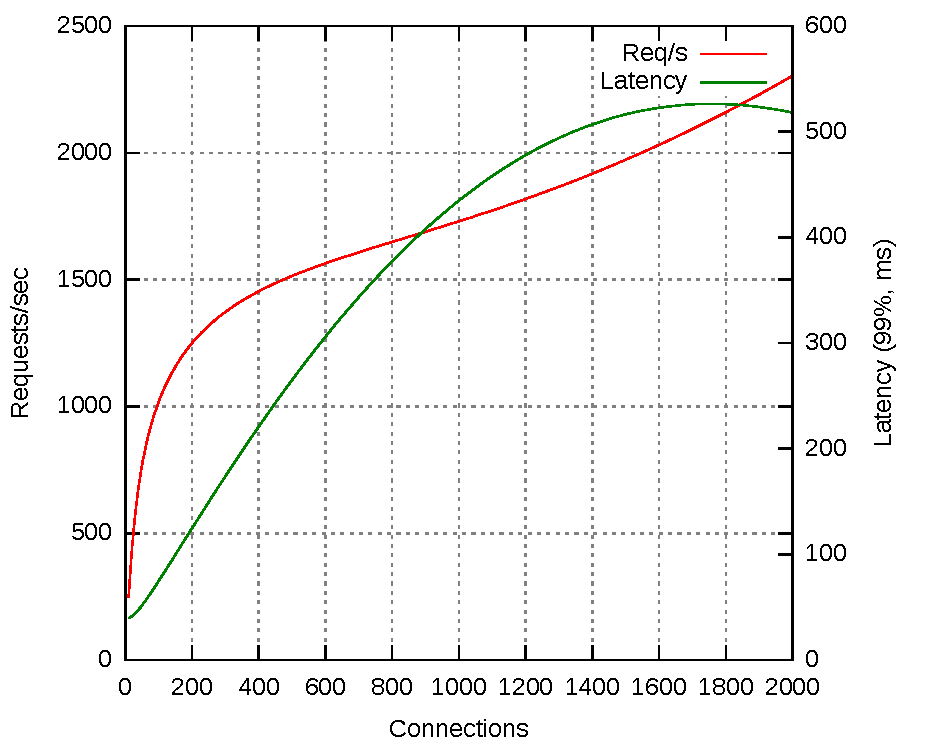
\includegraphics[width=0.6\textwidth]{figures/just-a-plot}
  \caption{Example vector figure in PDF.}
  \label{fig:vector}
\end{figure}



\section{Subfigures and subtables}
If a figure has multiple panels (subfigures), \texttt{subcaption} package is used to enable the correct references for subfigures.
Use \cmd{\fref}\marg{labstr} to refer to the full figure and \cmd{\fref}\marg{sublabstr} to refer to a specfic panel of that figure.
Use \cmd{\subcaptionref}\marg{sublabstr} to refer to just the panel number.
For example, \fref{fig:subfigure-demo} has two panels, \subcaptionref{fig:subfigdemo-cat} and \subcaptionref{fig:subfigdemo-dog}.
\fref{fig:subfigdemo-cat} refers to the cat panel.
This example explicitly creates the panel numbers since figures often have their panel numbers embedded.

\begin{figure}[t]
    \begin{subfigure}[b]{.5\linewidth}
        \centering
        \textbf{\sffamily A}\\[-0.5\onelineskip]
        \HUGE \emoji{cat}\\
        \emoji{cat-face}
        \phantomlabel{fig:subfigdemo-cat}
    \end{subfigure}%
    \begin{subfigure}[b]{.5\linewidth}
        \centering
        \textbf{\sffamily B}\\[-0.5\onelineskip]
        \HUGE \emoji{dog}\\
        \emoji{dog-face}
        \phantomlabel{fig:subfigdemo-dog}
    \end{subfigure}
    \caption[Two animals and their emojis.]{%
        Two animals and their emojis.
        \subref{fig:subfigdemo-cat} cats and \subref{fig:subfigdemo-dog} dogs.
    }
    \label{fig:subfigure-demo}
\end{figure}

Similarly, multiple tables can be grouped together as one using the same method. For example, see \tref{tab:subtable-demo}, which has two panels \subcaptionref{tab:subtab-a} and \subcaptionref{tab:subtab-b}.

\begin{table}[b]
    \centering
    \caption{Another table with two panels: \subref{tab:subtab-a} first and \subref{tab:subtab-b} second panel}
    \label{tab:subtable-demo}

    \begin{subtable}{0.5\linewidth}
        \centering
        \subcaption{First}\label{tab:subtab-a}
        \begin{tabular}{lc} \toprule
        A legendary table & 5 \\
        with two lines    & 6 \\ \bottomrule
        \end{tabular}
    \end{subtable}%
    \begin{subtable}{0.5\linewidth}
        \centering
        \subcaption{Second}\label{tab:subtab-b}
        \begin{tabular}{lc} \toprule
        A legendary table & 5 \\
        with two lines    & 6 \\ \bottomrule
        \end{tabular}
    \end{subtable}
\end{table}


\subsection{Figures with multiple panels merged into one source}
Sometimes the figure has already merges multiple panels and it's hard to split the panels into individual sources.
In this case, the panel numbers can be created using \cmd{\phantomlabel}\marg{labstr}.
For example, both \fref{fig:subfigure-demo} and \ref{fig:cell-cycle-mitosis} create panel numbers using this approach.


\subsection{Long figure legends spanning over the next page}
In some cases, the multi-panel figures may not have the vertical space to fit its legend, so the text overflow to the next page.
The text overflow can be achieved by using \cmd{\legendcontdnote} at the end of the first half of the legend (following the figure) and \cmd{\legendcontdref}\marg{labstr} at the beginning of the second half of the legend (usually at the next page).
\cmd{\legendcontdnote} inserts the ``\emph{(legend continued on next page)}'' mark right aligned at the end of the line or a new line.
\cmd{\legendcontdref} inserts the ``\emph{(Figure X continued)}'' mark.
Their style can modifyied by redefining the commands.

For example, \fref{fig:cell-cycle-mitosis} spans over two pages. Note how the two adjacent figure environments are constructed (and their figure placement specifiers).

\begin{figure}[p]
    \centering
    \phantomlabel{fig:mitosis-prophase}
    \phantomlabel{fig:mitosis-prometaphase}
    \phantomlabel{fig:mitosis-metaphase}
    \phantomlabel{fig:mitosis-anaphase}
    \phantomlabel{fig:mitosis-telophase}
    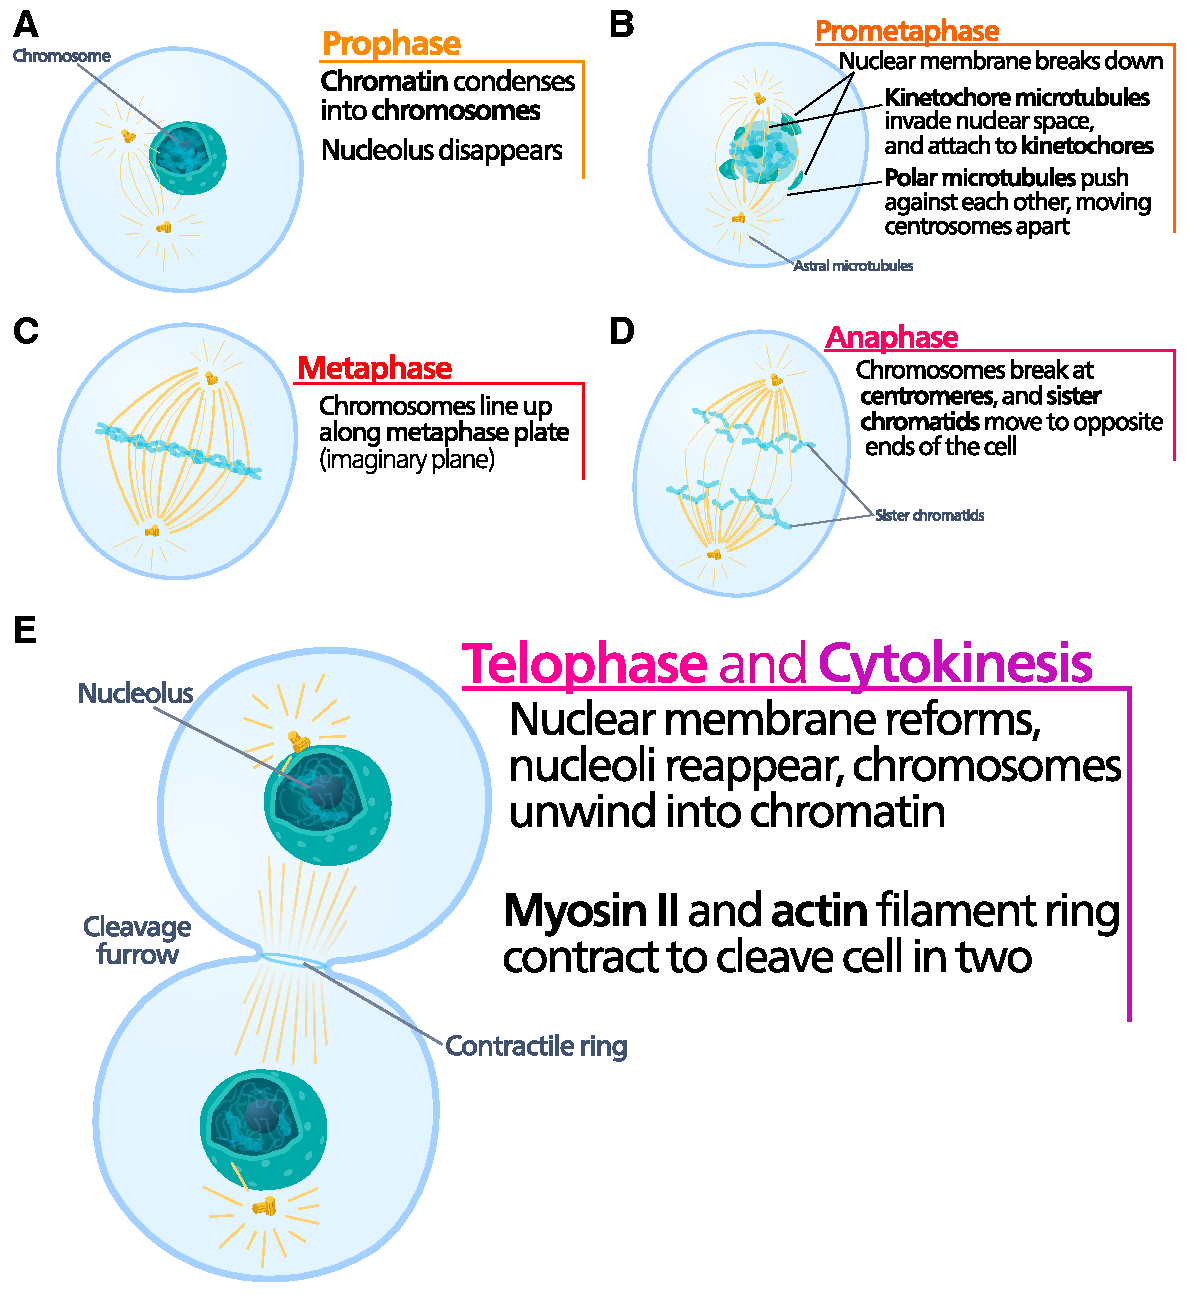
\includegraphics[width=\linewidth]{figures/cell-cycle-mitosis.pdf}
    \caption[Stages of mitotic phase of the cell cycle]{%
        Overview of different stages in the mitotic (M) phase of the animal cell cycle.
        Stages are defined based on the completion of a set of activities.
        \href{https://commons.wikimedia.org/wiki/File:Animal_cell_cycle-en.svg}{Figures} are made by Kelvin Ma (Kelvinsong; Kelvin13), \href{https://creativecommons.org/licenses/by/3.0}{CC BY 3.0}, via Wikimedia Commons.
        Text is copied from the \href{https://en.wikipedia.org/wiki/Mitosis}{Mitosis} page of Wikipedia.
        \subref{fig:mitosis-prophase}
        During prophase, which occurs after G\textsubscript{2} interphase,
        the cell prepares to divide by tightly condensing its chromosomes and initiating mitotic spindle formation.
        \subref{fig:mitosis-prometaphase}
        During prometaphase, the nuclear membrane breaks apart into numerous ``membrane vesicles'', and the chromosomes inside form protein structures called kinetochores.
        \legendcontdnote
    }
    \label{fig:cell-cycle-mitosis}
\end{figure}
\begin{figure}[t]
    \centering
    \legend{%
        \legendcontdref{fig:cell-cycle-mitosis}
        \subref{fig:mitosis-metaphase}
        During metaphase, the two centrosomes begin pulling the chromosomes towards opposite ends of the cell. The resulting tension causes the chromosomes to align along the metaphase plate or equatorial plane.
        \subref{fig:mitosis-anaphase}
        During anaphase, the replicated chromosomes are split and the newly-copied chromosomes are moved to opposite poles of the cell.
        \subref{fig:mitosis-telophase}
        During telophase, the effects of prophase and prometaphase (the nucleolus and nuclear membrane disintegrating) are reversed.
        Telophase is followed by cytokinesis, a separate process necessary for completing cell division.
    }
\end{figure}


\section{Tables}
Both examples (\tref{tab:include} and \ref{tab:nsf-sed}) use the \texttt{threeparttable} environment to format the table and allow table notes.
There are many packages available to manage tabular environments and they are generally compatible to this thesis document class.
For more sophisticated formattings, check out \texttt{memoir}'s documentation.

\begin{table}[tb]
    \centering
    \caption[Definite postgraduation commitments of doctorate recipients]{%
        Definite postgraduation commitments of doctorate recipients,
        by citizenship status and major field of study in 2019.
        Source: National Center for Science and Engineering Statistics, Survey of Earned Doctorates, National Science Foundation
        (\href{https://ncses.nsf.gov/pubs/nsf21308/}{link}; Table 51).
    }
    \label{tab:nsf-sed}
    \begin{threeparttable}[b]
    \begin{tabular}{llrrrrrrr@{}}
    \toprule
    Citizenship & Field & Total &
        Postdoc & Academia & Industry\tnote{a} & Other\tnote{b} & Abroad\\
    \midrule
    \multirow{3}{*}{\begin{tabular}[c]{@{}l@{}}All recipients\tnote{c}\end{tabular}}
        & Bio./biomed. & 5,054 &
            3,426 & 442 & 892 & 294 & 332 \\
        & Health & 1,525 &
            538	& 492 & 220 & 275 & 141\\
        & Comp./info. & 1,414 &
            276 & 254 & 789 & 95 & 161\\
    \midrule
    \multirow{3}{*}{\begin{tabular}[c]{@{}l@{}}U.S. citizen\\or PR\end{tabular}}
        & Bio./biomed. & 3,860 &
            2,536 & 385 & 679 & 260 & 118\\
        & Health & 1,248 &
            375 & 454 & 160 & 259 & 14\\
        & Comp./info. & 557 &
            102 & 133 & 247 & 75 & 23\\
    \midrule
    \multirow{3}{*}{\begin{tabular}[c]{@{}l@{}}Temporary\\visa holder\end{tabular}}
        & Bio./biomed. & 1,180 &
            882 & 55 & 212 & 31 & 213\\
        & Health & 275 &
            163 & 37 & 59 & 16 & 124\\
        & Comp./info. & 851 &
            173 & 120 & 540 & 18 & 136\\
    \bottomrule
    \end{tabular}
    \begin{tablenotes}
    \item[a] Includes doctorate recipients who indicated self-employment.
    \item[b] Includes doctorate recipients who indicated government, nonprofit, elementary or secondary school, or other employment and those with unknown employment.
    \item[c] Includes respondents who did not report citizenship status.
    \end{tablenotes}
    \end{threeparttable}
\end{table}


\section{Bibliography and Citations}
The \texttt{wustlthesis} document class itself does not implement any bibliography settings or styles, so any tool stack can be used together with it.

In this example, the bibliography is managed by \href{http://biblatex-biber.sourceforge.net/}{Biber} and \href{https://www.ctan.org/pkg/biblatex}{BibLaTeX} (not BibTeX), which support Unicode and more formatting options.
If \href{https://www.zotero.org/}{Zotero} is your reference manager, check out \href{https://retorque.re/zotero-better-bibtex/}{Better BibTeX} plugin for Zotero to enable more seamless integration with BibLaTex (and BibTeX).

Regardless of the tool stack in use, the citation commands should be the same, e.g., \cmd{\cite}\marg{key} and \cmd{\citeauthor}\marg{key}.
For example, this paper by \citeauthor{Jinek2012} demonstrated CRISPR can cut DNA at specific nucleotide sequences \cite{Jinek2012}.


\section{Equations}
See Equation~\ref{eq:maxwell}.

\begin{equation}
    \label{eq:maxwell}
    \begin{aligned}
    \frac{\partial\mathcal{D}}{\partial t} & = \nabla\times\mathcal{H},   & \text{(Loi de Faraday)}\\
    \frac{\partial\mathcal{B}}{\partial t} & = -\nabla\times\mathcal{E},  & \text{(Loi d'Ampère)}\\
    \nabla\cdot\mathcal{B}                 & = 0,                         & \text{(Loi de Gauss)}\\
    \nabla\cdot\mathcal{D}                 & = 0.                         & \text{(Loi de Colomb)}
    \end{aligned}
\end{equation}

\clearpage
\section{Page layout}
\layout


\begin{SingleSpace}
\printbibliography[title={References}]
\end{SingleSpace}

\appendix
\chapter{Appendix For Is a More Accessible Local Government a More Representative One? The Effects of Online Public Meetings}
\label{app:Chapter1}
\SingleSpacing*
\setSingleSpace{1.15}

    \section{Additional Sample Details:}
    Within the section below, I include details of my primary sample of local governments, including their names, socio-economic makeup, and meeting access over the course of my study.
    
    \subsection{Included Local Governments:}
    The subsection below details the local governments included within my sample. Meeting minutes were gathered from each government's official website or data repository.\\\\
    County:
    \begin{itemize}
      \item St. Louis County Government
    \end{itemize}
    Cities:
    \begin{multicols}{2}
      \begin{itemize}
        \item St. Ann
        \item Richmond Heights
        \item Kirkwood
        \item Ellisville
        \item Creve Coeur
        \item Brentwood
        \item Chesterfield
        \item Maplewood
        \item Ballwin
        \item Bridgeton
        \item Hazelwood
        \item Des Peres
        \item Manchester
      \end{itemize}
    \end{multicols}
    
  \noindent School Districts:
    \begin{multicols}{2}
    \begin{itemize}
      \item Parkway SD
      \item Kirkwood SD
      \item Brentwood SD
      \item Ferguson-Florissant SD
      \item Pattonville SD
      \item Hazelwood SD
      \item Ritenour SD
      \item Riverview Gardens SD
      \item Ladue SD
      \item Affton SD
      \item University City SD
      \item Clayton SD
      \item Rockwood SD
      \item Webster Groves SD
      \item Maplewood-Richmond Heights SD
    \end{itemize}
    \end{multicols}
    


    \subsection{Demographic Characteristics:}

    All of the following demographic estimates come from the 2020 American Community Survey.

    \begin{table}[H] \centering 
      \caption{Average Demographic Characteristics of Sample Governments} 
      \label{} 
      \scalebox{0.85}{\begin{tabular}{@{\extracolsep{5pt}} llll} 
    \\[-1.8ex]\hline 
    \hline \\[-1.8ex] 
    Variable & County & City & School \\ 
    \hline
    \\[-1.8ex] 
    Population & 1001982.00 &   21051.55 &   52118.20 \\ 
    Gender (F) & 47.77 & 47.51 & 47.68 \\ 
    White & 65.25 & 65.70 & 65.30 \\ 
    Black & 24.18 & 22.59 & 22.80 \\ 
    Asian & 4.55 & 4.87 & 5.12 \\ 
    Other & 1.36 & 1.79 & 1.67 \\ 
    Age (45+)  & 44.41 & 43.38 & 42.07 \\ 
    Education (College+) & 45.29 & 48.10 & 51.42 \\ 
    Median Income & 72562.00 & 81979.77 & 82670.27 \\ 
    Per Capita Income & 45307.00 & 46662.45 & 49951.33 \\ 
    Gini Index & 0.50 & 0.44 & 0.46 \\ 
    Median Structure Year & 1968 & 1966 & 1961 \\ 
    \hline \\[-1.8ex] 
    \end{tabular} }
    \end{table}

    \subsection{Access By Level of Government}
    \begin{figure}[H]
      \centering
       \text{Access to City Meetings From 2018-2021}\par\medskip
      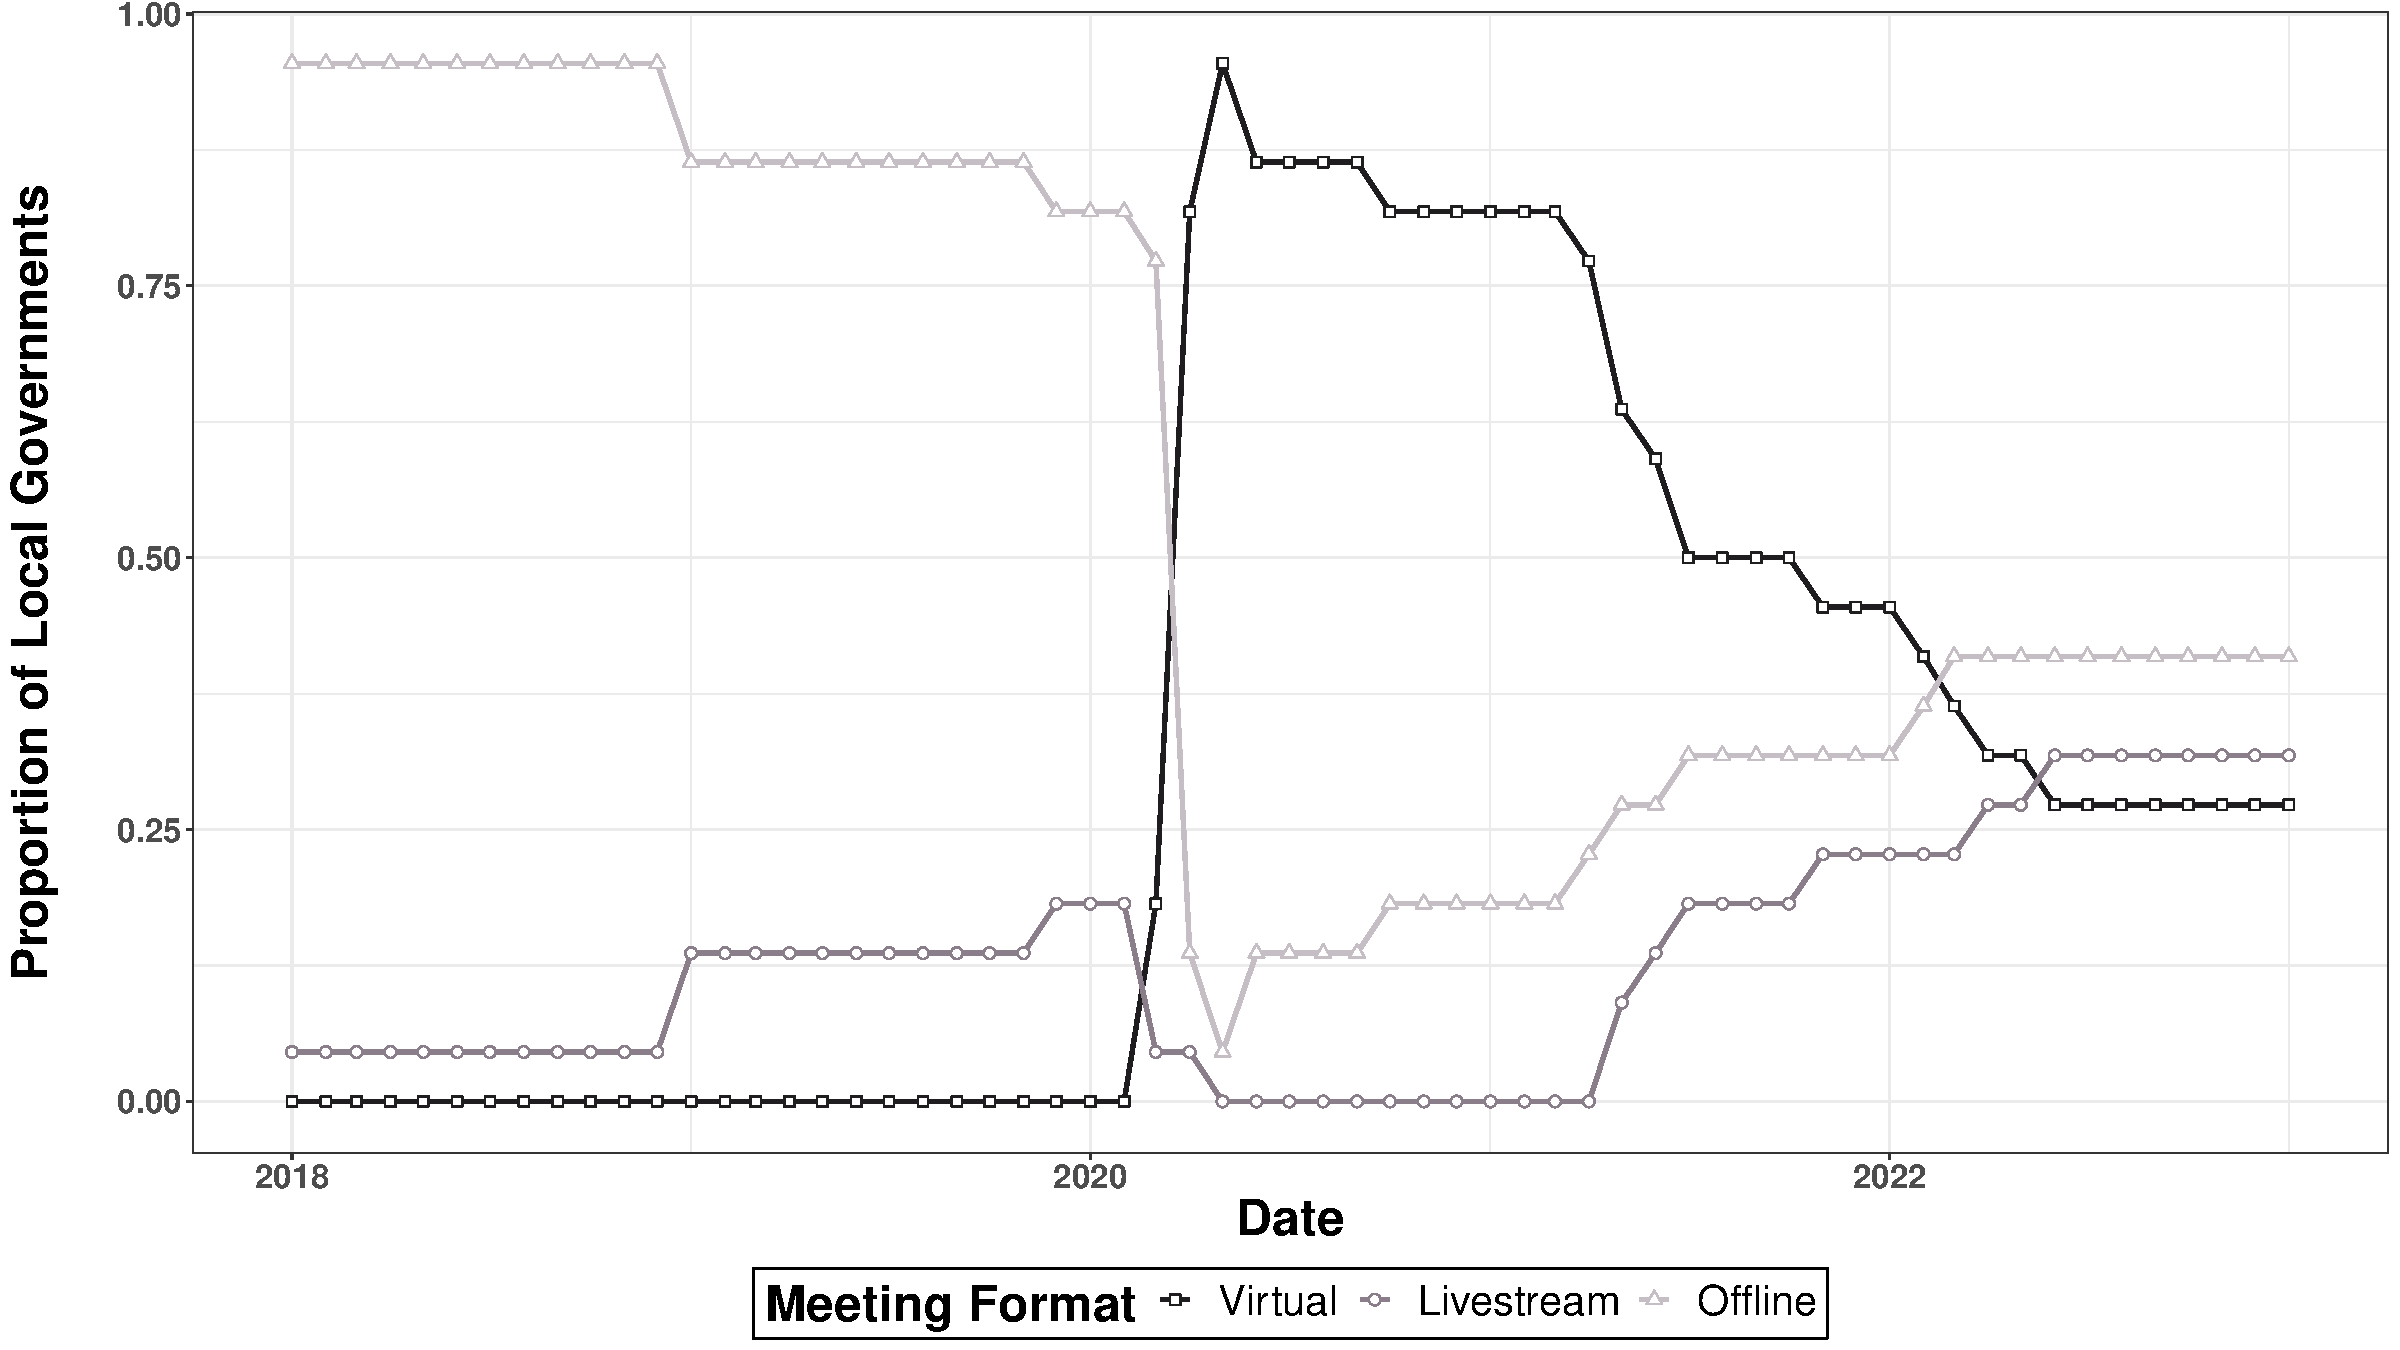
\includegraphics[scale=0.3]{Figures/CityAccess.pdf}
      \caption[Access to City Meetings From 2018-2021]{\footnotesize{Access to City Meetings From 2018-2021}}
      \label{}
  \end{figure}

  \begin{figure}[H]
    \centering
     \text{Access to School Board Meetings From 2018-2022}\par\medskip
    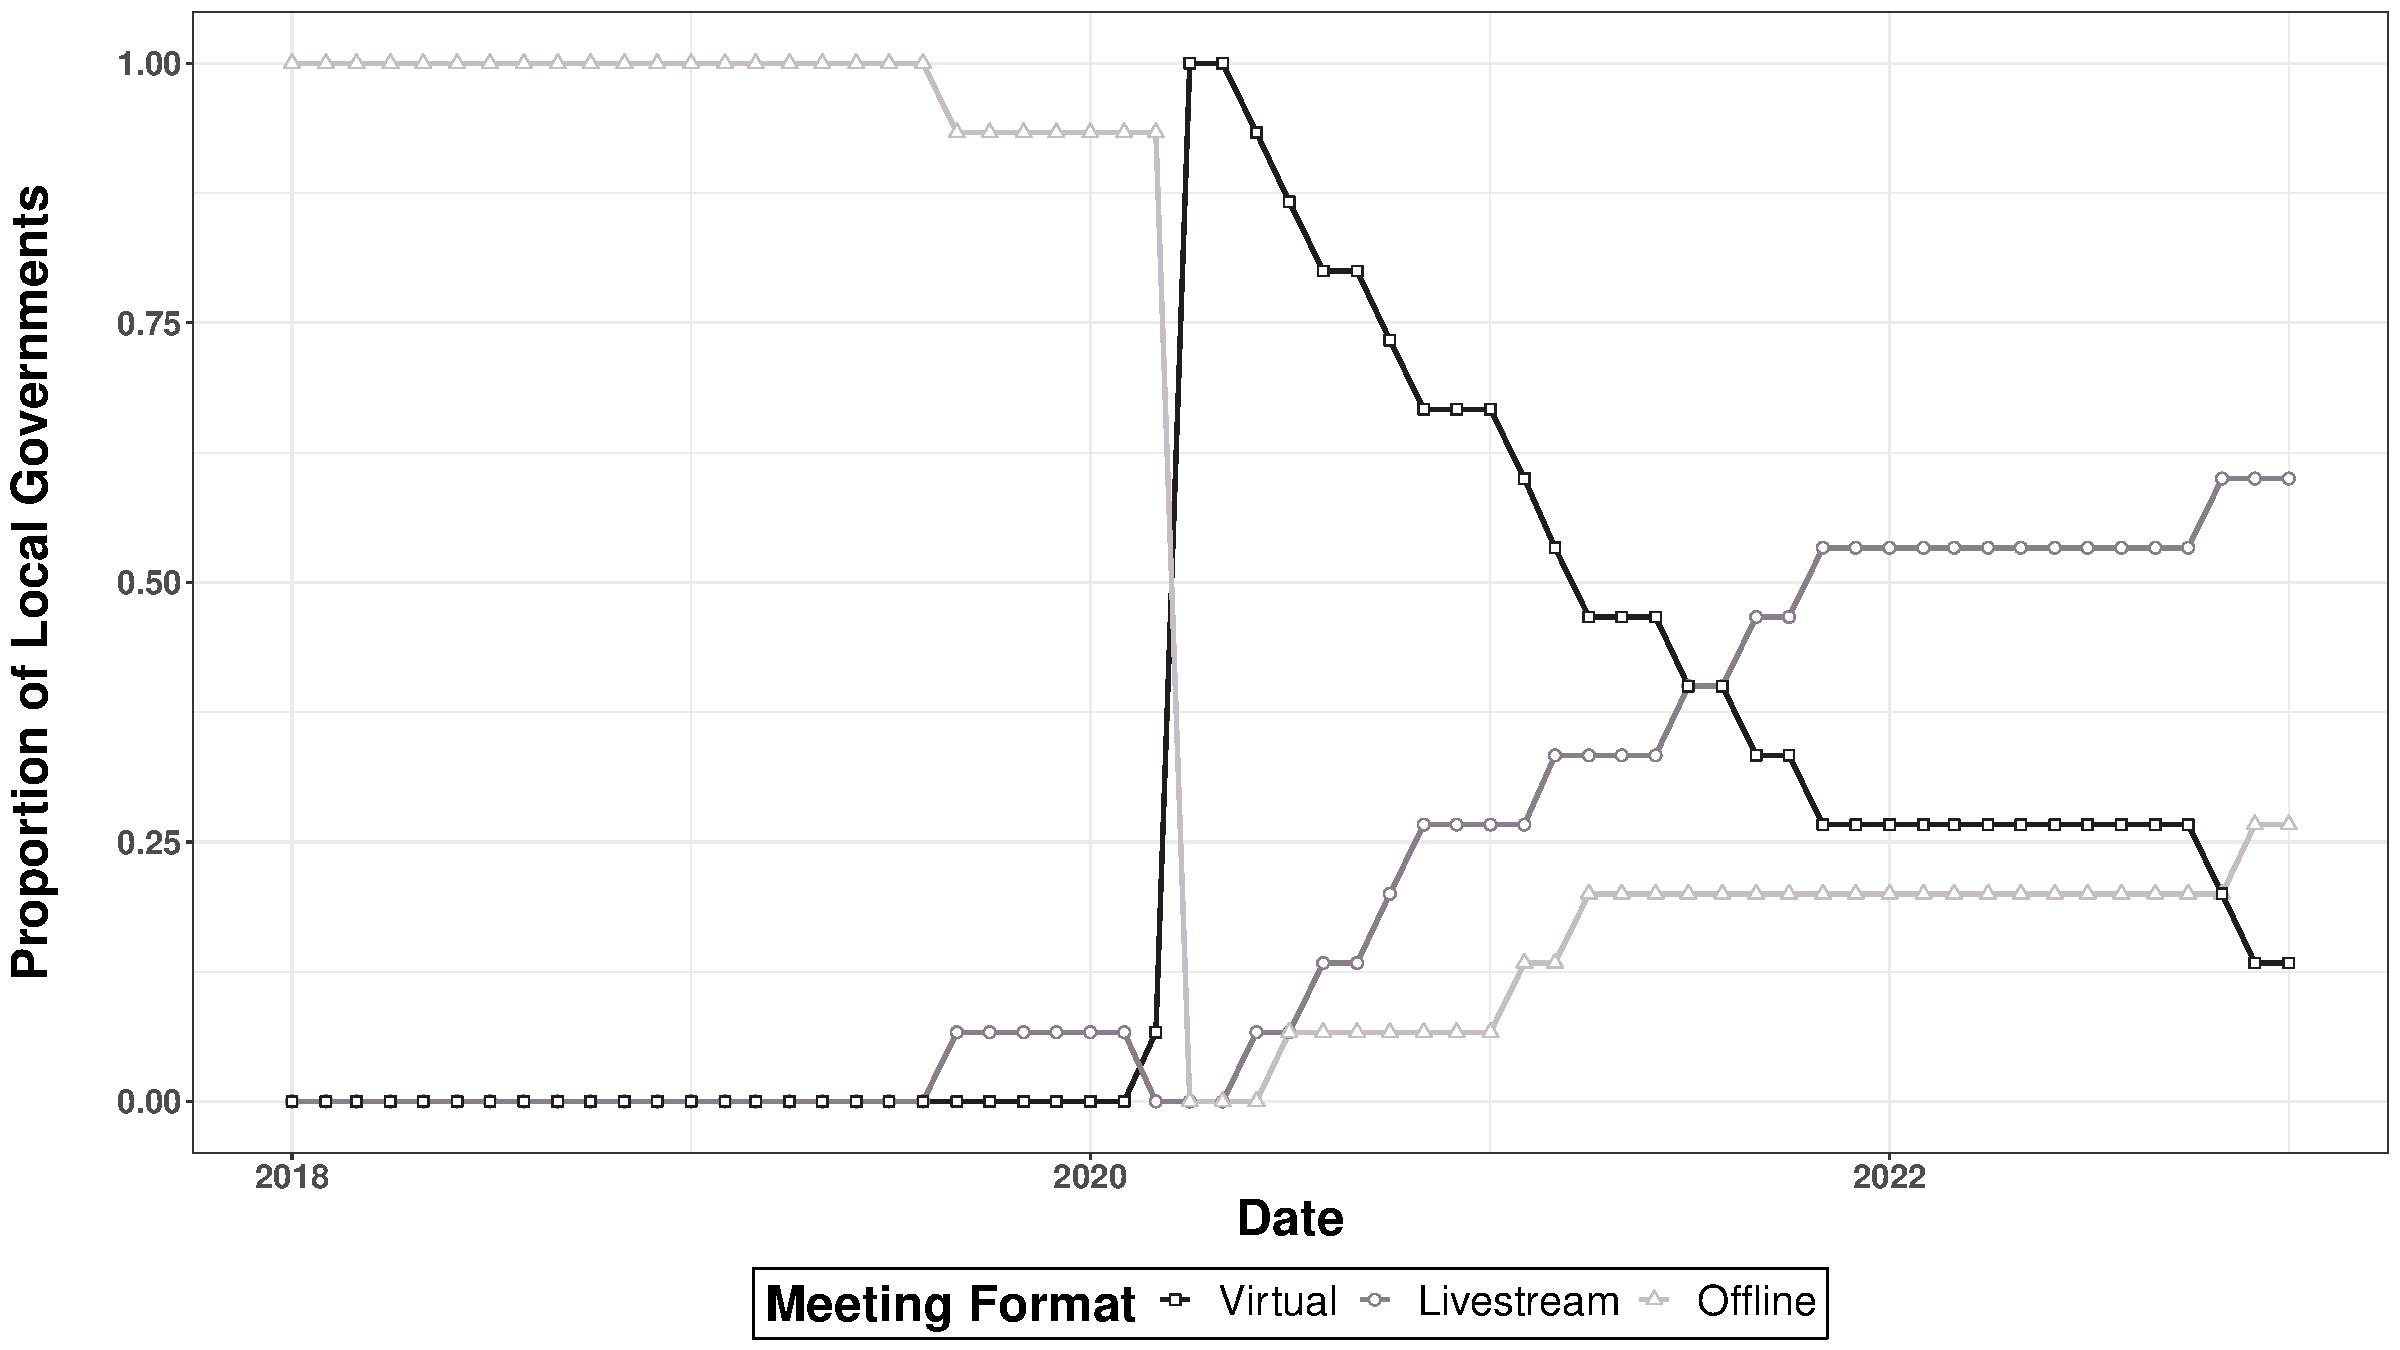
\includegraphics[scale=0.3]{Figures/SchoolAccess.pdf}
    \caption[Access to School Board Meetings From 2018-2022]{\footnotesize{}}
    \label{}
\end{figure}

\begin{figure}[H]
  \centering
   \text{Access to County Council Meetings From 2018-2022}\par\medskip
  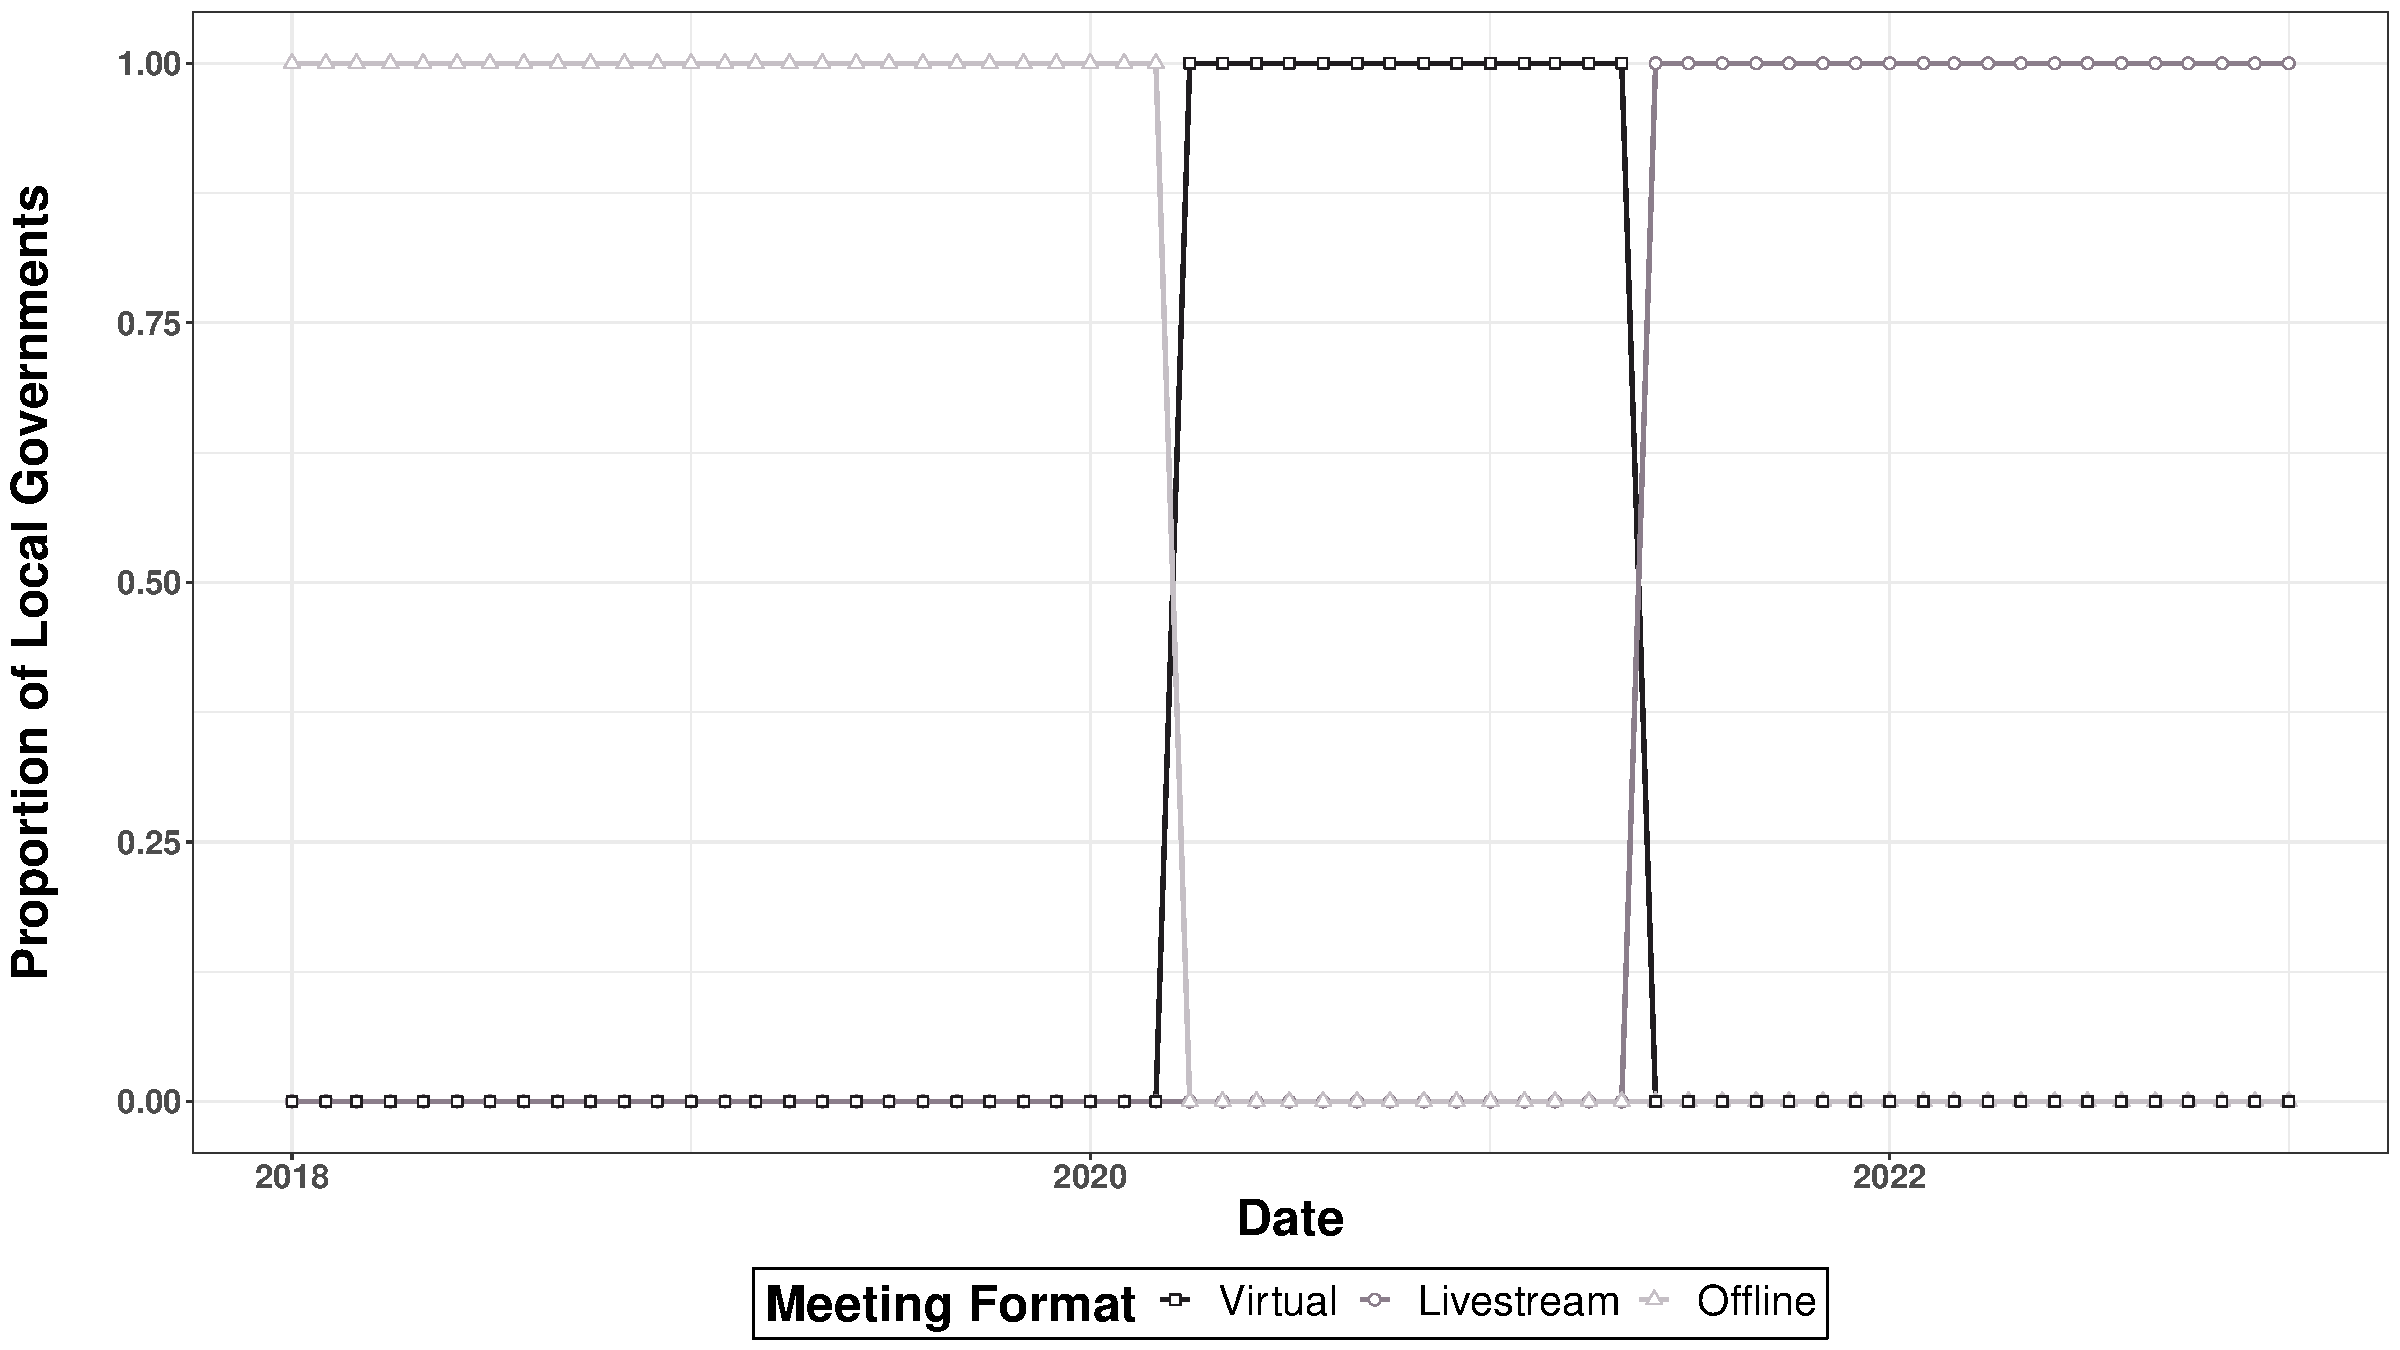
\includegraphics[scale=0.3]{Figures/CountyAccess.pdf}
  \caption[Access to County Council Meetings From 2018-2022]{\footnotesize{}}
  \label{}
\end{figure}




    \section{Full Tables For Figures:}
    \subsection{Figure 2 Regression Tables:}
    \begin{table}[H] \centering 
      \caption{Full Regression Results for Figure 2: Virtual} 
      \label{} 
      \scalebox{0.75}{\begin{tabular}{@{\extracolsep{5pt}}lcccc} 
    \\[-1.8ex]\hline \\[-1.8ex] 
    \\[-1.8ex] & \multicolumn{4}{c}{\textbf{Number of Commenters}} \\ 
     & \textbf{Pooled} & \textbf{County} & \textbf{School District} & \textbf{City} \\ 
    \hline \\[-1.8ex] 
     Virtual & 0.368$^{*}$ & $-$0.129 & 0.330 & 0.306 \\ 
      & (0.176) & (0.363) & (0.255) & (0.260) \\ 
      Constant & $-$0.968$^{*}$ & 3.707$^{*}$ & $-$1.904$^{*}$ & $-$0.019 \\ 
      & (0.415) & (0.240) & (0.673) & (0.449) \\ 
      \hline \\[-1.8ex] 
     Year FE &  & \ding{51}&  &  \\ 
    Month FE & \ding{51}&  & \ding{51}& \ding{51}\\ 
    Goverment FE & \ding{51}&  & \ding{51}& \ding{51}\\ 
    Num. Gov & 38 & 1 & 22 & 15 \\ 
    N & 1800 & 52 & 780 & 968 \\ 
    AIC & 5421.063 & 550.832 & 2614.811 & 2236.291 \\ 
    \hline \\[-1.8ex] 
    \multicolumn{5}{l}{$^{*}$p$<$0.05} \\ 
    \end{tabular} }
    \end{table} 

    \begin{table}[H] \centering 
      \caption{Full Regression Results for Figure 2: Livestreamed} 
      \label{} 
      \scalebox{0.75}{\begin{tabular}{@{\extracolsep{5pt}}lcccc} 
    \\[-1.8ex]\hline \\[-1.8ex] 
    \\[-1.8ex] & \multicolumn{4}{c}{\textbf{Number of Commenters}} \\ 
     & \textbf{Pooled} & \textbf{County} & \textbf{School District} & \textbf{City} \\ 
    \hline \\[-1.8ex] 
     Livestreamed & $-$0.137 & 1.139$^{*}$ & $-$0.363 & 0.261 \\ 
      & (0.178) & (0.528) & (0.256) & (0.290) \\ 
      Constant & $-$0.998$^{*}$ & 3.707$^{*}$ & $-$1.882$^{*}$ & $-$0.017 \\ 
      & (0.419) & (0.261) & (0.674) & (0.449) \\ \\
    \hline \\[-1.8ex] 
     Year FE &  & \ding{51}&  &  \\ 
    Month FE & \ding{51}&  & \ding{51}& \ding{51}\\ 
    Goverment FE & \ding{51}&  & \ding{51}& \ding{51}\\ 
    Num. Gov & 38 & 1 & 22 & 15 \\ 
    N & 1800 & 52 & 780 & 968 \\ 
    AIC & 5434.779 & 564.507 & 2614.505 & 2236.835 \\ 
    \hline \\[-1.8ex] 
    \multicolumn{5}{l}{$^{*}$p$<$0.05} \\ 
    \end{tabular} }
    \end{table} 

    \begin{table}[H] \centering 
      \caption{Full Regression Results for Figure 2: Online} 
      \label{} 
      \scalebox{0.75}{\begin{tabular}{@{\extracolsep{5pt}}lcccc} 
    \\[-1.8ex]\hline \\[-1.8ex] 
    \\[-1.8ex] & \multicolumn{4}{c}{\textbf{Number of Commenters}} \\ 
     & \textbf{Pooled} & \textbf{County} & \textbf{School District} & \textbf{City} \\ 
    \hline \\[-1.8ex] 
     Online & 0.246 & 2.483$^{*}$ & $-$0.050 & 0.293 \\ 
      & (0.181) & (0.566) & (0.346) & (0.203) \\ 
      Constant & $-$1.048$^{*}$ & 3.707$^{*}$ & $-$1.941$^{*}$ & $-$0.004 \\ 
      & (0.419) & (0.247) & (0.675) & (0.449) \\ \\
    \hline \\[-1.8ex] 
     Year FE &  & \ding{51}&  &  \\ 
    Month FE & \ding{51}&  & \ding{51}& \ding{51}\\ 
    Goverment FE & \ding{51}&  & \ding{51}& \ding{51}\\ 
    Num. Gov & 38 & 1 & 22 & 15 \\ 
    N & 1800 & 52 & 780 & 968 \\ 
    AIC & 5433.647 & 557.457 & 2616.083 & 2235.560 \\ 
    \hline \\[-1.8ex] 
    \multicolumn{5}{l}{$^{*}$p$<$0.05} \\ 
    \end{tabular} }
    \end{table} 



    \subsection{Figure 3 Regression Tables}
    \begin{table}[H]
      \centering
      \caption{Full Regession Results of Switching Away from Virtual Meetings}
      \scalebox{0.75}{\begin{tabular}{lccc}
        \hline\\[-1.8ex]
        \textbf{Group} & \textbf{Estimate} & \textbf{Std. Error} & \textbf{[95\% Pointwise Conf. Band]} \\
      \hline\\[-1.8ex]
      2 & -6.0815 & 1.8841 & [-9.7743, -2.3886]* \\
      3 & 4.4265 & 7.9697 & [-11.1939, 20.0469] \\
      4 & -8.5765 & 2.5928 & [-13.6583, -3.4946]* \\
      6 & -29.9583 & 3.5539 & [-36.9239, -22.9927]* \\
      7 & 1.4810 & 5.0879 & [-8.4911, 11.4530] \\
      10 & -2.0547 & 1.6289 & [-5.2472, 1.1378] \\
      11 & 1.4188 & 2.4016 & [-3.2883, 6.1259] \\
      13 & -0.7655 & 1.3506 & [-3.4126, 1.8816] \\
      15 & -0.4200 & 1.4075 & [-3.1786, 2.3386] \\
      17 & 4.6250 & 2.8540 & [-0.9688, 10.2188] \\
      19 & -11.5000 & 0.7413 & [-12.9529, -10.0471]* \\
      \hline 
      \hline
      \end{tabular}}
      \end{table}

      \begin{table}[H]
        \centering
        \caption{Full Regession Results of Switching Away from Online Meetings}
        \scalebox{0.75}{\begin{tabular}{lccc}
          \hline\\[-1.8ex]
          \textbf{Group} & \textbf{Estimate} & \textbf{Std. Error} & \textbf{[95\% Pointwise Conf. Band]} \\
        \hline\\[-1.8ex]
        3 & 1.2063 & 4.3231 & [-7.2669, 9.6794] \\
        10 & -2.6389 & 1.8715 & [-6.3070, 1.0292] \\
        13 & -2.5486 & 2.1956 & [-6.8519, 1.7547] \\
        \hline 
        \hline
        \end{tabular}}
        \end{table}
      


    \subsection{Figure 4 Regression Tables}
    \begin{table}[H]
      \centering
      \caption{Full Regession Results of Switching Away from Virtual Meetings}
      \scalebox{0.75}{\begin{tabular}{lccc}
        \hline\\[-1.8ex]
        \textbf{Group} & \textbf{Estimate} & \textbf{Std. Error} & \textbf{[95\% Pointwise Conf. Band]} \\
      \hline\\[-1.8ex]
      2 & -0.4765 & 0.9735 & [-2.4581, 1.5051] \\
      6 & 1.1591 & 0.2685 & [0.6124, 1.7057]* \\
      12 & 1.1461 & 0.3533 & [0.4270, 1.8652]* \\
      13 & -0.1097 & 0.4969 & [-1.1213, 0.9018] \\
      14 & -0.7552 & 0.7571 & [-2.2964, 0.7859] \\
      15 & 1.0909 & 1.4397 & [-1.8398, 4.0216] \\
      \hline 
      \hline
      \end{tabular}}
      \end{table}

    \begin{table}[H]
        \centering
        \caption{Full Regession Results of Switching Away from Online Meetings}
        \scalebox{0.75}{\begin{tabular}{lccc}
          \hline\\[-1.8ex]
          \textbf{Group} & \textbf{Estimate} & \textbf{Std. Error} & \textbf{[95\% Pointwise Conf. Band]} \\
        \hline\\[-1.8ex]
        2 & -0.4508 & 1.0045 & [-2.4292, 1.5276] \\
        6 & 1.2019 & 0.2565 & [0.6967, 1.7071]* \\
        12 & 1.2030 & 0.3007 & [0.6107, 1.7953]* \\
        13 & -0.2583 & 0.3845 & [-1.0156, 0.4990] \\
        15 & 0.7000 & 1.1169 & [-1.4998, 2.8998] \\
        \hline 
        \hline
        \end{tabular}}
        \end{table}

    \section{Supplementary Analyses:}
    \subsection{Simultaneous Comparisons of Commenters to Voters}
    \begin{table}[H] \centering 
      \caption{Pooled Commenters Compared to Voters} 
      \label{} 
    \scalebox{0.75}{\begin{tabular}{@{\extracolsep{5pt}}lcccc} 
    \\[-1.8ex]\hline 
    \hline \\[-1.8ex] 
     & \multicolumn{4}{c}{\textit{Dependent variable:}} \\ 
    \cline{2-5} 
    \\[-1.8ex] 
     & Pooled & County & City & School \\ 
    \\[-1.8ex] & (1) & (2) & (3) & (4)\\ 
    \hline \\[-1.8ex] 
     White & 0.177$^{*}$ & 0.154 & 0.259$^{*}$ & 0.106 \\ 
      & (0.062) & (0.081) & (0.128) & (0.149) \\ 
      & & & & \\ 
     Black & $-$0.089 & $-$0.028 & $-$0.493 & $-$0.144 \\ 
      & (0.121) & (0.164) & (0.378) & (0.219) \\ 
      & & & & \\ 
     Gender (F) & 0.492$^{*}$ & 0.760$^{*}$ & $-$0.171 & 0.805$^{*}$ \\ 
      & (0.046) & (0.064) & (0.088) & (0.120) \\ 
      & & & & \\ 
     Income (100K+) & 0.247$^{*}$ & 0.305$^{*}$ & 0.029 & 0.443$^{*}$ \\ 
      & (0.047) & (0.062) & (0.094) & (0.117) \\ 
      & & & & \\ 
     Education (HS+) & $-$0.048 & $-$0.068 & 0.157 & $-$0.172 \\ 
      & (0.058) & (0.077) & (0.123) & (0.136) \\ 
      & & & & \\ 
     Homeowner & 0.530$^{*}$ & 0.500$^{*}$ & 0.682$^{*}$ & 0.636$^{*}$ \\ 
      & (0.068) & (0.091) & (0.142) & (0.149) \\ 
      & & & & \\ 
     National Voter & 0.785$^{*}$ & 0.837$^{*}$ & 0.825$^{*}$ & 0.622$^{*}$ \\ 
      & (0.078) & (0.100) & (0.174) & (0.193) \\ 
      & & & & \\ 
     Local Voter & 1.104$^{*}$ & 0.860$^{*}$ & 1.403$^{*}$ & 1.439$^{*}$ \\ 
      & (0.048) & (0.062) & (0.104) & (0.123) \\ 
      & & & & \\ 
     Constant & $-$7.778$^{*}$ & $-$8.083$^{*}$ & $-$8.639$^{*}$ & $-$9.214$^{*}$ \\ 
      & (0.189) & (0.229) & (0.303) & (0.374) \\ 
      & & & & \\ 
    \hline \\[-1.8ex] 
    Zipcode FE & \ding{51}& \ding{51}& - & - \\ 
    City FE & - & - & \ding{51}& - \\ 
    School FE & - & - & - & \ding{51}\\ 
    Observations & 632,187 & 632,187 & 171,772 & 327,165 \\ 
    Akaike Inf. Crit. & 25,908.220 & 16,388.060 & 6,302.015 & 4,858.056 \\ 
    \hline 
    \hline \\[-1.8ex] 
    \textit{Note:}  & \multicolumn{4}{r}{$^{*}$p$<$0.05} \\ 
    \end{tabular} }
    \end{table} 

    \begin{table}[H] \centering 
      \caption{Online and Offline Commenters Compared to All Voters} 
      \label{} 
    \scalebox{0.75}{\begin{tabular}{@{\extracolsep{5pt}}lcccccccc} 
    \\[-1.8ex]\hline 
    \hline \\[-1.8ex] 
     & \multicolumn{8}{c}{\textit{Dependent variable:}} \\ 
    \cline{2-9} 
    \\[-1.8ex] 
     & \multicolumn{2}{c}{Pooled} & \multicolumn{2}{c}{County} & \multicolumn{2}{c}{City} & \multicolumn{2}{c}{School} \\ 
     
    \\[-1.8ex] & (Online) & (Offline) & (Online) & (Offline) & (Online) & (Offline) & (Online) & (Offline)\\ 
    \hline \\[-1.8ex] 
     White & 0.149 & 0.253$^{*}$ & 0.097 & 0.474$^{*}$ & 0.409 & 0.230 & 0.319 & $-$0.106 \\ 
      & (0.077) & (0.109) & (0.087) & (0.220) & (0.246) & (0.159) & (0.218) & (0.209) \\ 
      & & & & & & & & \\ 
     Black & $-$0.189 & 0.105 & $-$0.128 & 0.333 & $-$0.046 & $-$0.701 & $-$0.218 & 0.018 \\ 
      & (0.159) & (0.193) & (0.201) & (0.315) & (0.558) & (0.527) & (0.305) & (0.339) \\ 
      & & & & & & & & \\ 
     Gender (F) & 0.792$^{*}$ & 0.059 & 0.942$^{*}$ & 0.043 & $-$0.224 & $-$0.076 & 1.073$^{*}$ & 0.557$^{*}$ \\ 
      & (0.061) & (0.075) & (0.074) & (0.137) & (0.159) & (0.111) & (0.174) & (0.175) \\ 
      & & & & & & & & \\ 
     Income (100K+) & 0.325$^{*}$ & 0.130 & 0.383$^{*}$ & $-$0.100 & $-$0.080 & 0.133 & 0.351$^{*}$ & 0.531$^{*}$ \\ 
      & (0.059) & (0.082) & (0.068) & (0.158) & (0.172) & (0.119) & (0.158) & (0.177) \\ 
      & & & & & & & & \\ 
     Education (HS+) & $-$0.092 & 0.056 & $-$0.110 & 0.137 & 0.208 & 0.146 & $-$0.236 & $-$0.017 \\ 
      & (0.072) & (0.101) & (0.084) & (0.192) & (0.223) & (0.155) & (0.180) & (0.217) \\ 
      & & & & & & & & \\ 
     Homeowner & 0.577$^{*}$ & 0.411$^{*}$ & 0.590$^{*}$ & 0.181 & 0.630$^{*}$ & 0.658$^{*}$ & 0.624$^{*}$ & 0.667$^{*}$ \\ 
      & (0.087) & (0.109) & (0.105) & (0.181) & (0.242) & (0.180) & (0.200) & (0.233) \\ 
      & & & & & & & & \\ 
     National Voter & 0.755$^{*}$ & 0.849$^{*}$ & 0.778$^{*}$ & 1.145$^{*}$ & 0.778$^{*}$ & 0.907$^{*}$ & 0.650$^{*}$ & 0.538 \\ 
      & (0.094) & (0.144) & (0.108) & (0.259) & (0.296) & (0.228) & (0.246) & (0.324) \\ 
      & & & & & & & & \\ 
     Local Voter & 0.903$^{*}$ & 1.443$^{*}$ & 0.801$^{*}$ & 1.127$^{*}$ & 1.228$^{*}$ & 1.407$^{*}$ & 1.150$^{*}$ & 1.908$^{*}$ \\ 
      & (0.060) & (0.087) & (0.069) & (0.149) & (0.182) & (0.132) & (0.158) & (0.209) \\ 
      & & & & & & & & \\ 
     Constant & $-$8.088$^{*}$ & $-$9.405$^{*}$ & $-$8.183$^{*}$ & $-$24.595 & $-$10.272$^{*}$ & $-$9.290$^{*}$ & $-$9.580$^{*}$ & $-$10.911$^{*}$ \\ 
      & (0.222) & (0.391) & (0.241) & (410.557) & (0.600) & (0.391) & (0.469) & (0.717) \\ 
      & & & & & & & & \\ 
    \hline \\[-1.8ex] 
    Zipcode FE & \ding{51}& \ding{51}& \ding{51}& \ding{51}& - & - & - & - \\ 
    City FE & - & - & - & - & \ding{51}& \ding{51}& - & - \\ 
    School FE & - & - & - & - & - & - & \ding{51}& \ding{51}\\ 
    Observations & 632,187 & 632,187 & 632,187 & 632,187 & 171,772 & 171,772 & 327,165 & 327,165 \\ 
    Akaike Inf. Crit. & 17,646.340 & 10,154.080 & 13,628.920 & 3,802.738 & 2,261.061 & 4,212.815 & 2,921.446 & 2,248.457 \\ 
    \hline 
    \hline \\[-1.8ex] 
    \textit{Note:}  & \multicolumn{8}{r}{$^{*}$p$<$0.05} \\ 
    \end{tabular} }
    \end{table} 


    


    \section{Text-Analysis of Comments}
    \subsection{Examining the Content of Public Meeting Comments}
    In the following section I construct a separate STM model (K=20) for each level government within my sample (Roberts et al. 2019). Each model includes government and month level controls. For the county model, I replace government controls with zipcode controls. \autoref{tab:STMFull} presents the top 5 topics for each level of government.

    \begin{table}[H]
        \centering
        \caption{STM: Comment Topics By Level of Government}
        \label{tab:STMFull}
        \scalebox{.8}{
      \begin{tabular}{lll}
          \\[-1.8ex]\hline 
              \hline \\[-1.8ex] 
          \textbf{County Council}                            & \textbf{Municipal Council}                     & \textbf{School Board}                           \\
          \hline \\
          mask, mandat, counti,        & develop, light,       & comment, school,    \\
          wear, vaccin                 & traffic, concern      & chromebook, instruct \\ \\[-1.8ex]
          \hline\\
          sport, counti,        & spoke, propos,   & earn, virtual,  \\
          youth, page, support  & opposit, favor, rezon   & person, graduat, shorten\\ \\[-1.8ex]
          \hline\\
          school, kid,          & contract, renew,          & propos, oppos,     \\
          play, children, team & trash, waste & rezon, concern, spoke \\ \\[-1.8ex]
          \hline\\
          prosecuti, judge,  & concern, construct, & return, school,    \\
          attorney, file, process &  express, sidewalk & staff, online, learn \\ \\[-1.8ex]
          \hline\\
          project, develop,      & maryland, trail,        & spoke, regard,  \\
          tax, propos, resid &    thank, event & favor, concern, kirkwood\\ \\[-1.8ex]
          \\[-1.8ex]\hline 
              \hline \\[-1.8ex]                                  
          \end{tabular}
      }
    \end{table}

    
    Next I follow the same procedure but subset each level of my sample by whether a meeting was accessibile online or not. I then reconstruct a model for each subset across each level of government. \autoref{tab:county_online_offline}, \autoref{tab:city_online_offline}, and \autoref{tab:school_online_offline} display the top four topics for online and offline comments at the county, city, and school district levels. While the exact topics change between online and offline meetings, most topics appear jurisdictionally relevant to their respective level of government. 
    
    
    
    \begin{table}[H]
        \centering
        \caption{County Topics of Online Versus Offline Comments}
        \label{tab:county_online_offline}
        \scalebox{0.8}{
        \begin{tabular}{l|l}
        \hline\\
        \textbf{Online} & \textbf{Offline} \\ \\[-1.8ex]
        \hline\\
        mask, mandat, vaccin, counti, pleas & employe, counti, year, work, servic \\
        & \\ \\[-1.8ex]
                  \hline\\
        sport, play, counti, loui, school & anim, volunt, dog, shelter, counti \\
        & \\\\[-1.8ex]
                  \hline\\
        counti, bill, council, page, power & counti, loui, council, execut, meet \\
        & \\\\[-1.8ex]
                  \hline\\
        counti, loui, tax, propos, properti & tax, million, counti, loui, zoo \\
        & \\\\[-1.8ex]
                  \hline
        \end{tabular}}
        
        \end{table}
        
        \begin{table}[H]
        \centering
        \caption{City Topics of Online Versus Offline Comments}
        \label{tab:city_online_offline}
        \scalebox{0.8}{
        \begin{tabular}{l|l}
        \hline\\
        \textbf{Online} & \textbf{Offline} \\ \\[-1.8ex]
        \hline\\
        council, address, street, highland, terrac & spoke, propos, opposit, comment, concern \\
        & \\ \\[-1.8ex]
                  \hline\\
        state, propos, oppos, develop, favor & develop, concern, oppos, state, traffic \\
        & \\\\[-1.8ex]
                  \hline\\
        van, mark, way, space, rezon & ask, council, citi, servic, note, approach \\
        & \\\\[-1.8ex]
                  \hline\\
        food, unhous, support, mini, pantri & polic, protest, charg, galleria, peac \\
        & \\\\[-1.8ex]
                  \hline
        \end{tabular}}
        
        \end{table}
        
        \begin{table}[H]
        \centering
        \caption{School Board Topics of Online Versus Offline Comments}
        \label{tab:school_online_offline}
        \scalebox{0.8}{
        \begin{tabular}{l|l}
        \hline\\
        \textbf{Online} & \textbf{Offline} \\ \\[-1.8ex]
        \hline\\
        patron, comment, total, various, read & gender, ident, ave, geyer, kepling \\
        & \\ \\[-1.8ex]
                  \hline\\
        graduat, ask, student, parent, ceremoni & comment, polici, kelli, meet, advoc \\
        & \\\\[-1.8ex]
                  \hline\\
        learn, virtual, comment, return, -person & school, spoke, high, pattonvill, student \\
        & \\\\[-1.8ex]
                  \hline\\
        school, year, plan, involv, back--school & board, educ, spoke, member, regard \\
        & \\\\[-1.8ex]
                  \hline\\
        \end{tabular}}
        
        \end{table}

        \subsection{Do Online Meetings Elicit More Negative Comments?}
        Beyond the topics of the comments, I also examine whether online meetings elicit more negative comments. To analyze this, I calculate each comment's average sentence level VADER sentiment scores and scale it between -1 and 1 \citep{Hutto_Gilbert_2014}. Overall, average sentiment for Offline (0.100) and Online (0.099) meetings are both positive, but not statistically different.


\begin{figure}[H]
    \centering
    \caption{Average Comment Sentiment By Meeting Format}
    \label{fig:Sentiment}
    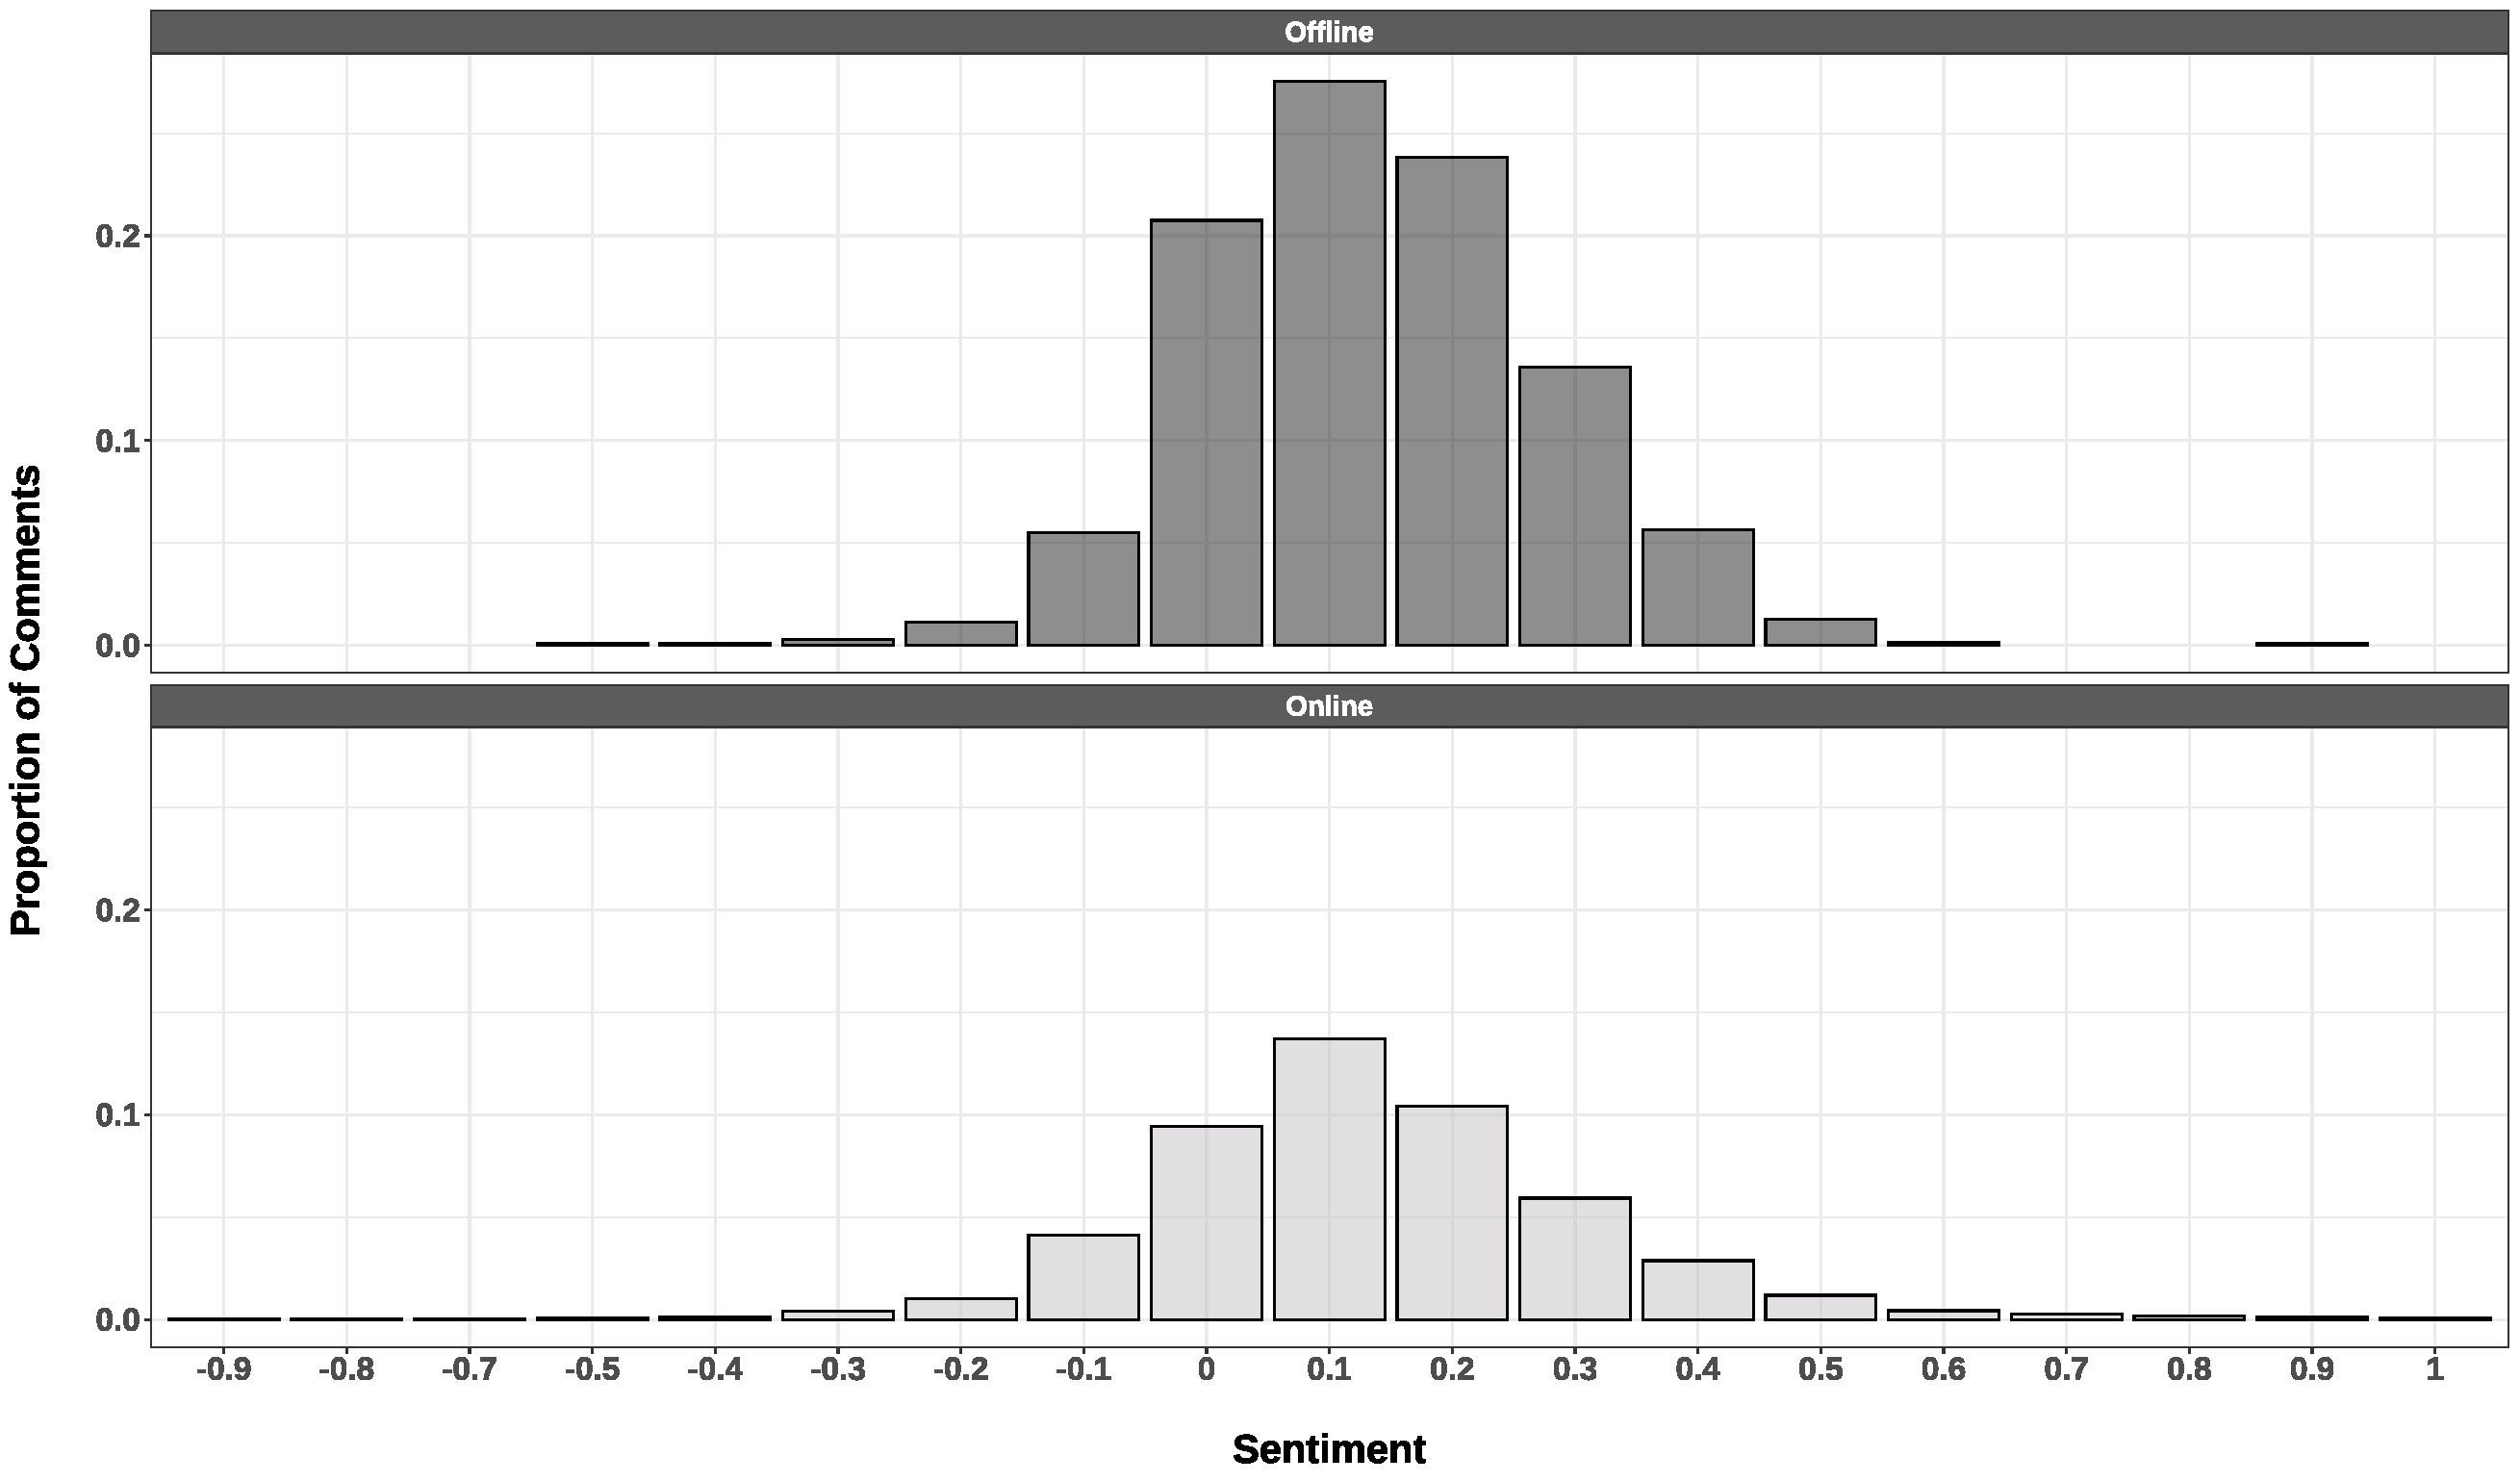
\includegraphics[scale=0.35]{Figures/Sentiment.pdf}
\end{figure}



    
    
    \section{Survey Details:}
    \subsection{Question Wording:}

    \small
      \noindent \textbf{Non-Meeting Attendees:} What best describes why you haven't attended a local political meeting (such as school district or city council) this past year?
      \begin{enumerate}
        \item Inconvenient meeting times
        \item No compelling reason or issue
        \item Unable to join the meeting (either in-person or virtually)
        \item Didn’t know how to attend meetings
        \item Didn’t want to attend meetings alone
        \item Voiced concerns in an alternative way (email, phone call, etc.)
        \item Other (please specify)
      \end{enumerate}


      \noindent \textbf{Meeting Attendees:} What best describes why you attended a local political meeting (such as school district or city council) this past year?
      \begin{enumerate}
        \item Support a specific policy issue.
        \item Oppose a specific policy issue.
        \item Voice an opinion or concern.
        \item Thank a local public official.
        \item Critique a local public official.
        \item Observe the meeting
        \item Other (please specify)
      \end{enumerate}


    \subsection{Survey Responses:}

    \begin{figure}[H]
      \centering
       \text{}\par\medskip
      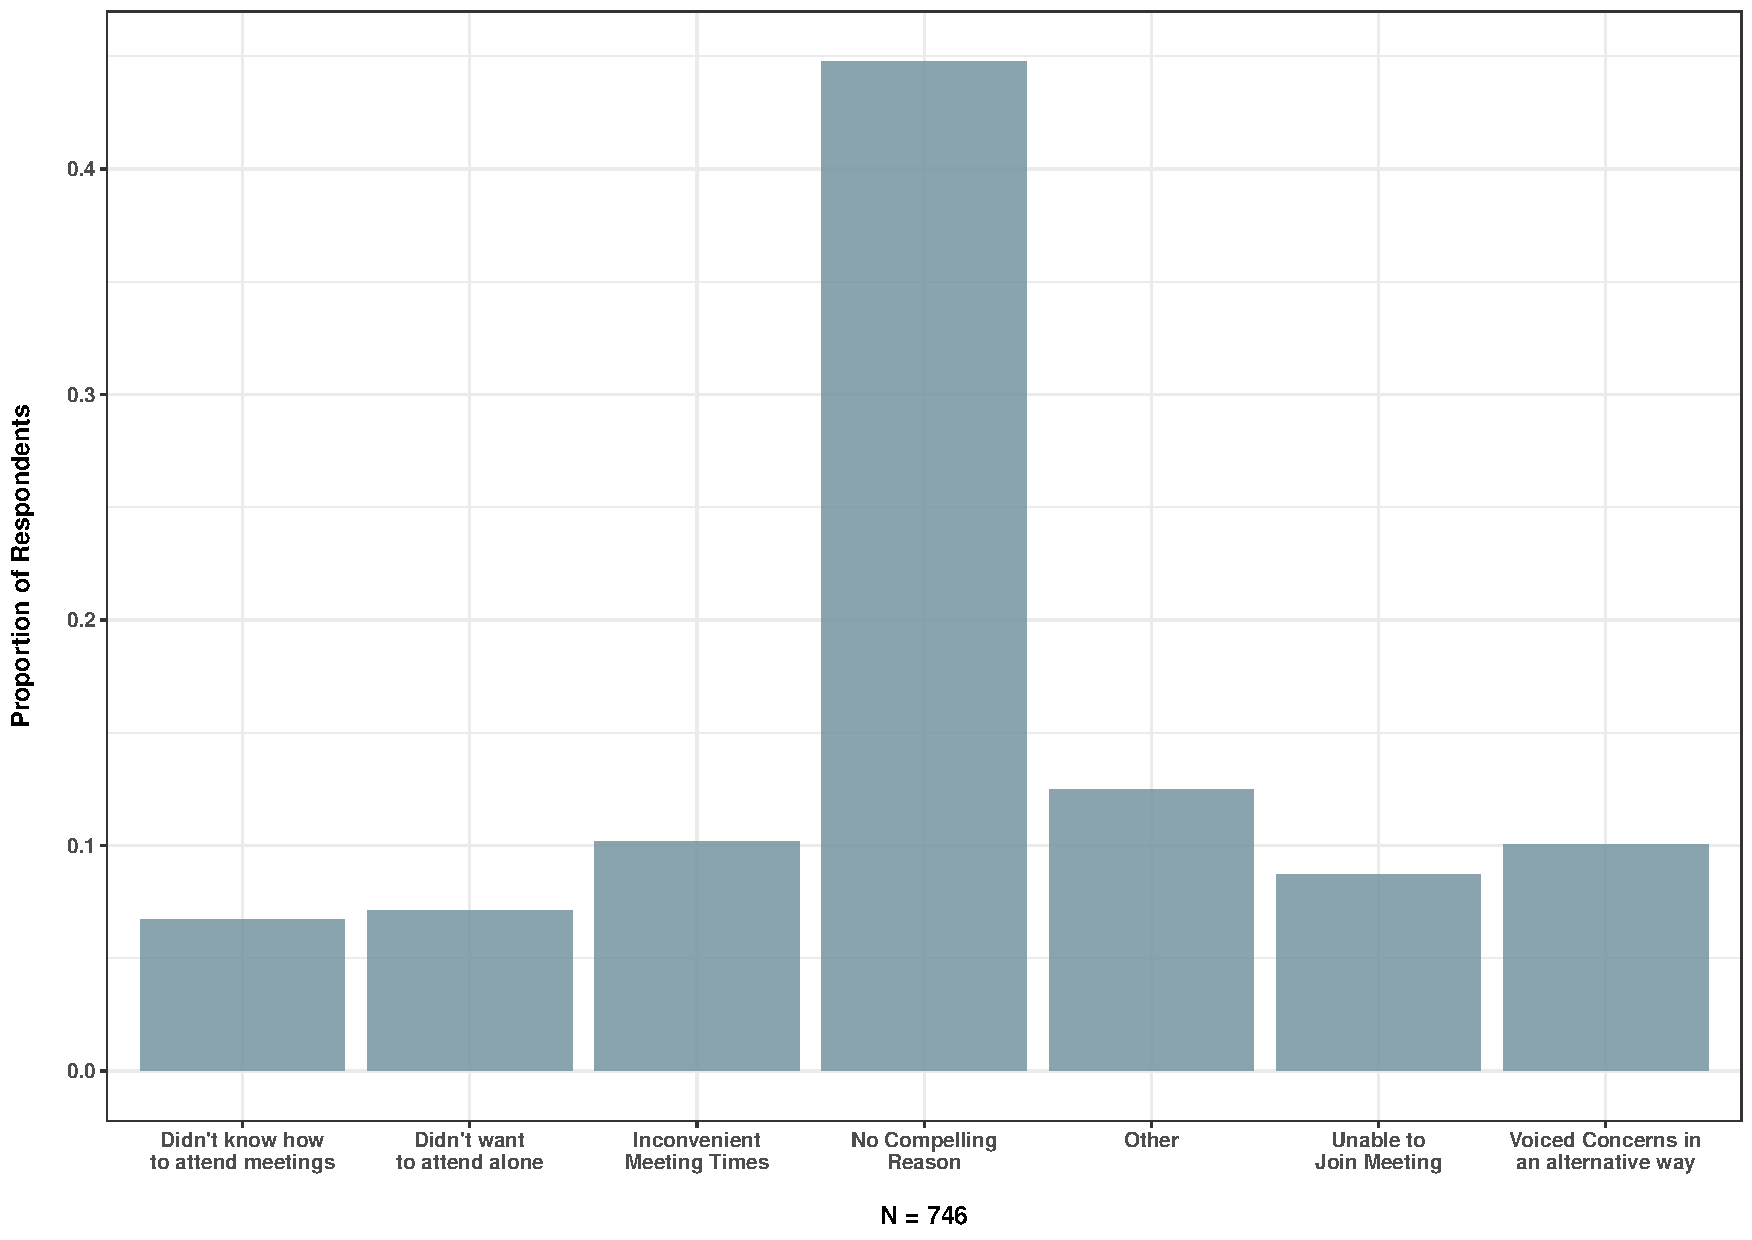
\includegraphics[scale=0.43]{Figures/CCESNoMeeting.pdf}
      \caption[Response to Non-Meeting Attendees Question]{\footnotesize{Response to Non-Meeting Attendees Question}}
      \label{}
    \end{figure}


    \begin{figure}[H]
      \centering
       \text{}\par\medskip
      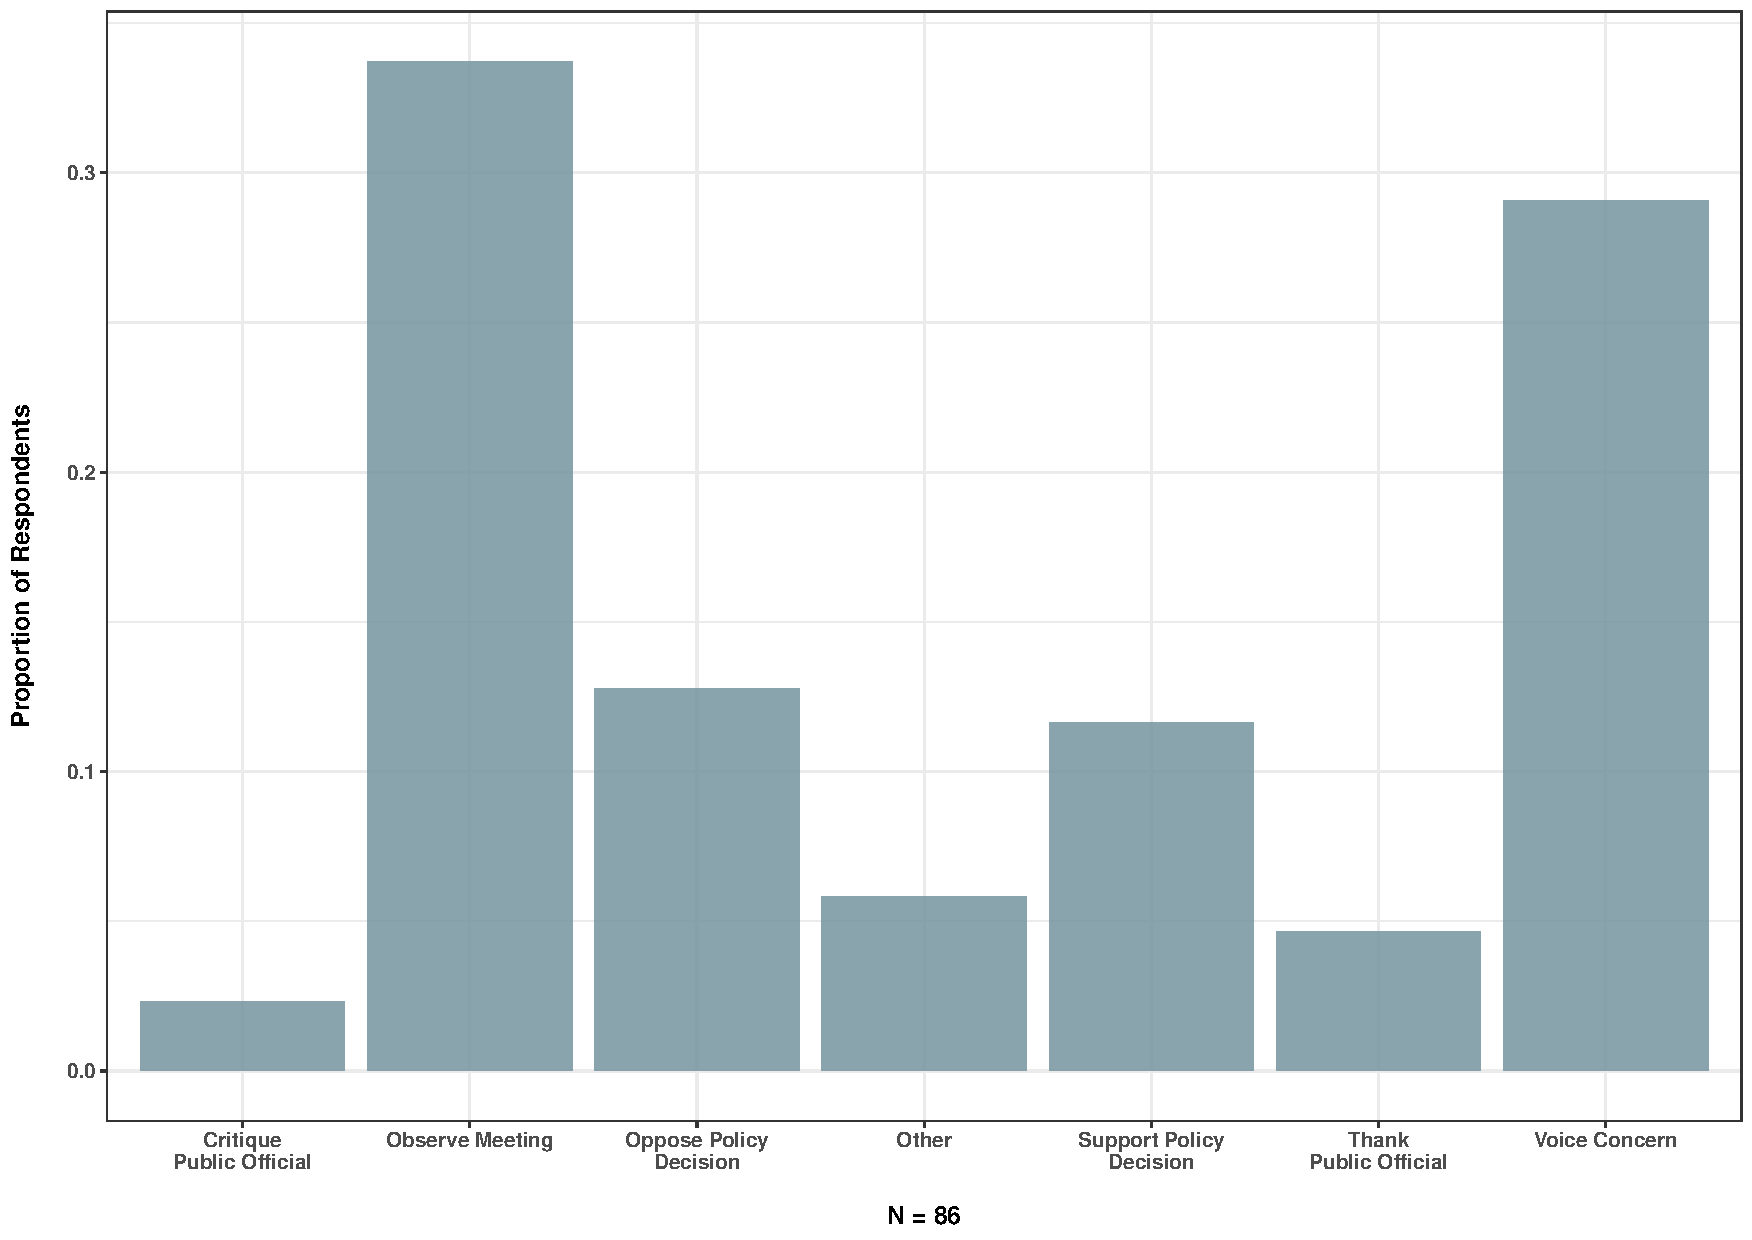
\includegraphics[scale=0.43]{Figures/CCESMeeting.pdf}
      \caption[Response to Meeting Attendees Question]{\footnotesize{Response to Meeting Attendees Question}}
      \label{}
    \end{figure}
\chapter{Appendix For Is it All Good in the Neighborhood? How Partisanship May Shape Evaluations of Municipal Services}
\label{app:Chapter2}
\SingleSpacing*
\setSingleSpace{1}


\section{Survey Details}
\subsection{Variable Distributions}
\begin{table}[H] \centering 
  \caption{Descriptive Statistics of Independent and Dependent Variables: Full CCES} 
  \label{} 
  \scalebox{0.8}{
\begin{tabular}{@{\extracolsep{5pt}} cccccc} 
\\[-1.8ex]\hline 
\hline \\[-1.8ex] 
 & Mean & Median & SD & Min & Max \\ 
\hline \\[-1.8ex] 
Individual Covariates: &&&&&\\
\hline\\
Age & $48.680$ & $49$ & $17.608$ & $18$ & $93$ \\ 
Gender (M) & $0.445$ & $0$ & $0.497$ & $0$ & $1$ \\ 
Parent & $0.658$ & $1$ & $0.475$ & $0$ & $1$ \\ 
Republican & $0.377$ & $0$ & $0.485$ & $0$ & $1$ \\ 
Independent & $0.139$ & $0$ & $0.346$ & $0$ & $1$ \\ 
Black & $0.079$ & $0$ & $0.270$ & $0$ & $1$ \\ 
Hispanic & $0.087$ & $0$ & $0.282$ & $0$ & $1$ \\ 
Asian & $0.029$ & $0$ & $0.169$ & $0$ & $1$ \\ 
Homeowner & $0.622$ & $1$ & $0.485$ & $0$ & $1$ \\ 
Income & $6.412$ & $6$ & $3.306$ & $1$ & $16$ \\ 
Rural & $0.150$ & $0$ & $0.357$ & $0$ & $1$ \\ \\
Objective Measures: &&&&&\\
\hline\\
School Rating & $2.651$ & $2.605$ & $0.826$ & $0$ & $5$ \\ 
Crime Rate (2018) & $482.325$ & $300.771$ & $534.689$ & $0$ & $3,063.617$ \\ 
Crime Rate (2017) & $576.387$ & $355.356$ & $658.426$ & $0$ & $13,124.290$ \\ 
Crime Rate Difference & $-97.506$ & $-27.720$ & $259.851$ & $-2,013.473$ & $1,195.273$ \\ \\
Service Evaluations: &&&&&\\
\hline\\
School & $0.335$ & $0$ & $0.998$ & $-2$ & $2$ \\ 
Police & $0.458$ & $0$ & $0.931$ & $-2$ & $2$ \\ 
\hline \\[-1.8ex] 
\end{tabular} }
\end{table} 

\begin{table}[H] \centering 
  \caption{Difference in Covariate Means Between CCES and Large Cities Subset} 
  \label{} 
\begin{tabular}{@{\extracolsep{5pt}} lcccc} 
\\[-1.8ex]\hline 
\hline \\[-1.8ex] 
 & CCES & Large City Subset & $\Delta$ & P-Value \\ 
\hline \\[-1.8ex] 
Demographics: &&&&\\
\hline
Age & 48.667 & 46.537 & 2.130 & 0 \\ 
Gender (M) & 0.451 & 0.459 & -0.008 & 0.156 \\ 
Parent & 0.654 & 0.572 & 0.082 & 0 \\ 
Black & 0.091 & 0.145 & -0.054 & 0 \\ 
Hispanic & 0.080 & 0.124 & -0.044 & 0 \\ 
Asian & 0.028 & 0.041 & -0.013 & 0 \\ 
Homeowner & 0.630 & 0.536 & 0.094 & 0 \\ 
Rural Res. & 0.191 & 0.030 & 0.160 & 0 \\
Income & 6.520 & 6.530 & -0.010 & 0.786 \\\\
Partisanship: &&&&\\
\hline
Republican & 0.385 & 0.279 & 0.106 & 0 \\ 
Independent & 0.122 & 0.111 & 0.011 & 0.001 \\\\
Objective Measures: &&&&\\
\hline
School Rating & 2.628 & 2.271 & 0.357 & 0 \\ 
Violent Crime Rate & 82.940 & 69.789 & 13.151 & 0 \\ 
Property Crime Rate & 462.579 & 395.580 & 66.999 & 0 \\ 
\hline \\[-1.8ex] 
\end{tabular} 
\begin{tablenotes}
    \item {\footnotesize Note: The above table presents results of a two sample t-test between the 2018 CCES and the new merged data set. Covariates such as Republican, Independent, and Black are coded as a binary choice.Income (1-10) is measured on its own categorical scale.Crime rates are standardized to incidents per 100,000 citizens.}
\end{tablenotes}
\end{table} 


\section{Supplemental Analyses}
\subsection{Full Regression Results For Table 1}

\begin{table}[H] \centering 
    \SingleSpacing*
  \caption{OLS Regression of Local School and Police Evaluations on Partisan Identity: Full Results} 
  \label{}
  \scalebox{0.65}{
\begin{tabular}{@{\extracolsep{5pt}}lcc} 
\\[-1.8ex]\hline 
\hline \\[-1.8ex] 
 & \multicolumn{2}{c}{\textit{Service Evaluation:}} \\ 
\cline{2-3} 
\\[-1.8ex] & Police & School \\ 
\hline \\[-1.8ex] 
 Republican & $0.264^{*}$ & -0.035 \\ 
  & (0.018) & (0.028) \\ 
  & & \\ 
 Property Crime Rate & 0.00000 &  \\ 
  & (0.00003) &  \\ 
  & & \\ 
 Violent Crime Rate & $-0.0004^{*}$ &  \\ 
  & (0.0001) &  \\ 
  & & \\ 
 School Rating &  & $0.340^{*}$ \\ 
  &  & (0.014) \\ 
  & & \\
 Age & $0.007^{*}$ & 0.0002 \\ 
  & (0.0005) & (0.001) \\ 
  & & \\ 
 Gender (M) & 0.004 & $0.034^{*}$ \\ 
  & (0.010) & (0.011) \\ 
  & & \\ 
 Parent & 0.018 & $0.087^{*}$ \\ 
  & (0.012) & (0.015) \\ 
  & & \\ 
 Education & $0.013^{*}$ & 0.006 \\ 
  & (0.005) & (0.004) \\ 
  & & \\ 
 Rural Res. & $-0.175^{*}$ & -0.028 \\ 
  & (0.018) & (0.017) \\ 
  & & \\ 
 Homeowner & $0.053^{*}$ & $0.032^{*}$ \\ 
  & (0.012) & (0.015) \\ 
  & & \\ 
 Black & $-0.282^{*}$ & -0.016 \\ 
  & (0.033) & (0.035) \\ 
  & & \\ 
 Hispanic & $-0.038^{*}$ & 0.040 \\ 
  & (0.015) & (0.027) \\ 
  & & \\ 
 Asian & 0.060 & $0.118^{*}$ \\ 
  & (0.046) & (0.048) \\ 
  & & \\ 
 Income & $0.025^{*}$ & $0.016^{*}$ \\ 
  & (0.002) & (0.002) \\ 
  & & \\ 
\hline \\[-1.8ex] 
State Fixed Effects & \ding{51}& \ding{51}\\
Observations & 29,020 & 34,812 \\ 
$R^{2}$ & 0.078 & 0.103 \\ 
Adjusted $R^{2}$ & 0.076 & 0.101 \\ 
F Statistic & 187.880 (df = 13; 28958) & 332.247 (df = 12; 34749) \\ 
\hline 
\hline \\[-1.8ex] 
\end{tabular}} 
\begin{tablenotes}
    \item {\footnotesize Note: The above table presents the results of a OLS regression with state fixed effects and clustered standard errors. Crime rates are standardized to incident per 100,000 citizens. Standard errors are presented in parentheses.$^{*}$p$<$0.05}
\end{tablenotes}
\end{table} 

\begin{table}[H] \centering 
    \SingleSpacing*
  \caption{Hierarchical Linear Regression of Local Roads  Evaluation on Partisan Identity: Full Results} 
  \label{} 
  \scalebox{0.7}{
\begin{tabular}{@{\extracolsep{5pt}}lc} 
\\[-1.8ex]\hline 
\hline \\[-1.8ex] 
 & \multicolumn{1}{c}{\textit{Service Evaluation:}} \\ 
\cline{2-2} 
\\[-1.8ex] & Roads \\ 
\hline \\[-1.8ex] 
  Republican & 0.030 \\ 
  & (0.026) \\ 
  & \\ 
 Traffic Index & $-$0.003 \\ 
  & (0.003) \\ 
  & \\ 
 Age & $-0.005^{*}$ \\ 
  & (0.001) \\ 
  & \\ 
 Gender (M) & 0.020 \\ 
  & (0.022) \\ 
  & \\ 
 Parent & $0.049^{*}$ \\ 
  & (0.024) \\ 
  & \\ 
 Education & 0.016\\ 
  & (0.008) \\ 
  & \\ 
 Rural & $-0.102$ \\ 
  & (0.095) \\ 
  & \\ 
 Homeowner & $0.075^{*}$ \\ 
  & (0.025) \\ 
  & \\ 
 Black & $-0.175^{*}$ \\ 
  & (0.033) \\ 
  & \\ 
 Hispanic & $-0.019$ \\ 
  & (0.036) \\ 
  & \\ 
 Asian & $-0.036$ \\ 
  & (0.056) \\ 
  & \\ 
 Income & $0.016^{*}$ \\ 
  & (0.004) \\ 
  & \\ 
 Constant & $-0.003$ \\ 
  & (0.077) \\ 
  & \\ 
\hline \\[-1.8ex] 
Observations & 6,928 \\ 
State Random Effects & \ding{51}\\ 
Municipality Random Effects & \ding{51}\\
AIC & 18,191.980 \\ 
\hline 
\hline \\[-1.8ex] 
\end{tabular} }
\begin{tablenotes}
    \item {\footnotesize Note: The above table presents the results of a hierarchical linear regression with random effects. All respondents are nested within municipalities within states. Standard errors are presented in parentheses.$^{*}$p$<$0.05}
\end{tablenotes}
\end{table} 


\subsection{Alternative Modeling Specifications}

\begin{table}[H] \centering 
    \SingleSpacing*
  \caption{OLS Regression of Local School and Police Evaluations on Partisan Identity: Full Results and Independents} 
  \label{} 
  \scalebox{0.7}{
\begin{tabular}{@{\extracolsep{5pt}}lcc} 
\\[-1.8ex]\hline 
\hline \\[-1.8ex] 
 & \multicolumn{2}{c}{\textit{Service Evaluation:}} \\ 
\cline{2-3} 
\\[-1.8ex] & Police & School \\ 
\hline \\[-1.8ex] 
 Republican & $0.261^{*}$ & -0.037 \\ 
  & (0.018) & (0.028) \\ 
  & & \\ 
 Independent & $-0.048^{*}$ & $-0.185^{*}$ \\ 
  & (0.018) & (0.021) \\ 
  & & \\ 
 Property Crime Rate & -0.00000 &  \\ 
  & (0.00003) &  \\ 
  & & \\ 
 Violent Crime Rate & $-0.0004^{*}$ &  \\ 
  & (0.0001) &  \\ 
  & & \\ 
 School Rating &  & $0.341^{*}$ \\ 
  &  & (0.013) \\ 
  & & \\ 
 Age & $0.007^{*}$ & 0.0003 \\ 
  & (0.0004) & (0.001) \\ 
  & & \\ 
 Gender (M) & -0.001 & $0.029^{*}$ \\ 
  & (0.009) & (0.011) \\ 
  & & \\ 
 Parent & 0.021 & $0.089^{*}$ \\ 
  & (0.011) & (0.014) \\ 
  & & \\ 
 Education & $0.012^{*}$ & 0.004 \\ 
  & (0.005) & (0.004) \\ 
  & & \\ 
 Rural Res. & $-0.165^{*}$ & -0.020 \\ 
  & (0.017) & (0.016) \\ 
  & & \\ 
 Homeowner & $0.055^{*}$ & $0.034^{*}$ \\ 
  & (0.013) & (0.014) \\ 
  & & \\ 
 Black & $-0.289^{*}$ & -0.022 \\ 
  & (0.033) & (0.032) \\ 
  & & \\ 
 Hispanic & $-0.046^{*}$ & 0.048 \\ 
  & (0.014) & (0.026) \\ 
  & & \\ 
 Asian & 0.073& $0.115^{*}$ \\ 
  & (0.040) & (0.044) \\ 
  & & \\ 
 Income & $0.026^{*}$ & $0.017^{*}$ \\ 
  & (0.002) & (0.002) \\ 
  & & \\ 
\hline \\[-1.8ex] 
Observations & 32,994 & 39,548 \\ 
$R^{2}$ & 0.078 & 0.106 \\ 
Adjusted $R^{2}$ & 0.077 & 0.104 \\ 
\hline 
\hline \\[-1.8ex] 
\end{tabular} }
\begin{tablenotes}
    \item {\footnotesize Note: The above table presents the results of a OLS regression with state fixed effects and clustered standard errors. Crime rates are standardized to incident per 100,000 citizens. Standard errors are presented in parentheses.$^{*}$p$<$0.05}
\end{tablenotes}
\end{table} 


\subsection{Alternative Model Specifications}
\begin{table}[H] \centering 
    \SingleSpacing*
  \caption{Hierarchical Linear Regression of 7-Point Party ID on Local School and Police Evaluations} 
  \label{} 
  \scalebox{0.7}{
\begin{tabular}{@{\extracolsep{5pt}}lcc} 
\\[-1.8ex]\hline 
\hline \\[-1.8ex] 
 & \multicolumn{2}{c}{\textit{Service Evaluation:}} \\ 
\cline{2-3} 
\\[-1.8ex] & Police & School \\ 
\hline \\[-1.8ex] 
 Party ID & 0.050$^{*}$ & $-$0.010$^{*}$ \\ 
  & (0.002) & (0.002) \\ 
  & & \\ 
 Crime Rate & $-$0.0001$^{*}$ &  \\ 
  & (0.00001) &  \\ 
  & & \\ 
 School Rating &  & 0.321$^{*}$ \\ 
  &  & (0.007) \\ 
  & & \\ 
 Age & 0.007$^{*}$ & 0.0005 \\ 
  & (0.0003) & (0.0003) \\ 
  & & \\ 
 Gender (M) & $-$0.006 & 0.023$^{*}$ \\ 
  & (0.010) & (0.010) \\ 
  & & \\ 
 Parent & 0.013 & 0.086$^{*}$ \\ 
  & (0.011) & (0.011) \\ 
  & & \\ 
 Education & 0.013$^{*}$ & 0.004 \\ 
  & (0.004) & (0.003) \\ 
  & & \\ 
 Income & 0.025$^{*}$ & 0.017$^{*}$ \\ 
  & (0.002) & (0.002) \\ 
  & & \\ 
 Rural & $-$0.179$^{*}$ & $-$0.045$^{*}$ \\ 
  & (0.013) & (0.013) \\ 
  & & \\ 
 Homeowner & 0.051$^{*}$ & 0.030$^{*}$ \\ 
  & (0.012) & (0.011) \\ 
  & & \\ 
 Black & $-$0.251$^{*}$ & 0.002 \\ 
  & (0.020) & (0.018) \\ 
  & & \\ 
 Hispanic & $-$0.032 & 0.057$^{*}$ \\ 
  & (0.020) & (0.019) \\ 
  & & \\ 
 Asian & 0.069$^{*}$ & 0.118$^{*}$ \\ 
  & (0.032) & (0.030) \\ 
  & & \\ 
 Constant & $-$0.254$^{*}$ & $-$0.682$^{*}$ \\ 
  & (0.031) & (0.044) \\ 
  & & \\ 
\hline \\[-1.8ex] 
State Fixed Effects & \ding{51}& \ding{51}\\ 
Municipality Fixed Effects & \ding{51}& \ding{51}\\
Observations & 32,994 & 39,548 \\ 
AIC & 86,091.060 & 106,191.300 \\ 
\hline 
\hline \\[-1.8ex] 
\end{tabular} }
\begin{tablenotes}
    \item {\footnotesize Note: The above table presents the results of a hierarchical linear regression with random effects. All respondents are nested within municipalities within states. Standard errors are presented in parentheses.$^{*}$p$<$0.05}
\end{tablenotes}
\end{table} 

\begin{table}[H] \centering 
  \caption{Hierarchical Regression Results With Alternative Measures of Police Performance} 
  \label{} 
  \scalebox{0.9}{
\begin{tabular}{@{\extracolsep{5pt}}lcc} 
\\[-1.8ex]\hline 
\hline \\[-1.8ex] 
\\[-1.8ex] & (1) & (2)\\ 
\hline \\[-1.8ex] 
 2017 Crime Rate & 0.00001 &  \\ 
  & (0.00003) &  \\ 
  & & \\ 
 2018 Crime Rate & $-$0.0001$^{*}$ &  \\ 
  & (0.00004) &  \\ 
  & & \\ 
 Crime Rate Difference &  & 0.00000 \\ 
  &  & (0.00003) \\ 
  & & \\ 
 Constant & $-$0.138$^{*}$ & $-$0.186$^{*}$ \\ 
  & (0.031) & (0.030) \\ 
  & & \\ 
\hline \\[-1.8ex] 
State Fixed Effects & \ding{51}& \ding{51}\\ 
Municipality Fixed Effects & \ding{51}& \ding{51}\\
Additional Controls & \ding{51}& \ding{51}\\
Observations & 32,115 & 32,115 \\ 
AIC & 83,722.270 & 83,730.040 \\ 
\hline 
\hline \\[-1.8ex] 
\end{tabular} }
\begin{tablenotes}
    \item {\footnotesize Note: The above table presents the results of a hierarchical linear regression with random effects. Model (1) includes both current and lagged crime rates. Model (2) includes only the year change in crime rates. All respondents are nested within municipalities within states. Standard errors are presented in parentheses.$^{*}$p$<$0.05}
\end{tablenotes}
\end{table}


\chapter{Appendix For Utilizing Large Language Models To Transform Messy Text-Based Sources In Useful Data}
\label{app:Chapter3}
\SingleSpacing*
\setSingleSpace{1}


\section{Example Applications}

\subsection{Local Meeting Minutes:}
The following section displays a selection of meeting minute excerpts and their resulting output from OpenAI's GPT 3.5 model. For each example, I prompted the model with the prompt displayed within the body of the main paper and then fed the entirety of the meeting text from which the excerpt originated into the model.


\begin{figure}[H]
\centering
\textbf{Meeting Text Excerpt \#1}\par\medskip
\begin{lstlisting}[label={lst:brief-text}]
Middle school math teacher Megan Grossbauer, received the district's 
Excellence in Education Award for leadership and contributions 
to the learning environment for students in the district. Those 
in attendance viewed a video of Mrs. Grossbauer filmed by high 
school teacher Don Goble.

Turning to the superintendent's remarks, Dr. Wipke congratulated 
Megan on her well-deserved recognition and talked about his recent 
podcast recording which included Megan. Dr.Wipke went on to share brief 
updates related to the transition back to in-person learning for
students and plans to remain aligned with St. Louis County Health 
Department recommendations as COVID-19 trends appear to be increasing. 
Dr. Wipke also highlighted the recent design meeting hosted by several 
architect team members from Ittner and Perkins & Will. Dr. Wipke 
commended Sue Blumm and her foodservice team for their quick planning 
to ensure all meals served at Old Bonhomme were uninterrupted as they 
were faced with a boil order last week.

President Jaeger called for Board committee reports. 
Dr. Buckner reported on the Finance and Facilities Board Advisory 
Committees.

President Jaeger called for superintendent committee reports. 
Dr. Buckner reported on the Superintendent's Finance 
and Facilities Committee.

One patron, Andy Cohen, addressed the Board during the time period 
set aside for public comments regarding agenda and non-agenda items.

Turning to the action agenda, Mrs. Jaeger called for a 
motion to approve the evening's consent agenda. On a motion 
by Mr. Johnson, seconded by Dr. Goldstein, the following
resolution passed on a vote of 7-0:
\end{lstlisting}
\caption[Meeting Text Example \#1]{Sample School District Meeting Text From Ladue School District}
\end{figure}


\begin{figure}[H]
\centering
\textbf{Model Output:}\par\medskip
\begin{lstlisting}[language=python]
{
"Name": ["Andy Cohen"],
"Address": ["NA"],
"Comment": ["Comment regarding agenda and non-agenda items"]
}
\end{lstlisting}
\caption[Meeting Text Example Output \#1]{Formatted output from the LLM}
\end{figure}

\begin{figure}[H]
\centering
\textbf{Meeting Text Excerpt \#2}\par\medskip
\begin{lstlisting}[]
3. ANNOUNCEMENTS
3.01 Student Representative Announcements
Ms. Jaiden Smith was not present.
3.02 Superintendent's Announcements
Dr. Hardin-Bartley read superintendent announcements.
4. CITIZEN COMMENTS
4.01 Citizen Comments
e Stacy Brown- surplus property
e Maureen Axelbaum- surplus property
e Nicole Adewale- surplus property
e Jacqueline Stack- surplus property
e Colleen Dille- surplus property
e Roma Trousdale- surplus property
e Aaren Ginsburg- surplus property
e Lori Yudovich- surplus property
e Yvette Joy Liebesman, 7570 Cornell Avenue- surplus property
e Steven McMahon- surplus property
e Mark Tubbs- surplus property
e Meg A Ullman- surplus property
e Kim Field- surplus property
5. CONSENT AGENDA
5.01 Approval of the Consent Agenda
\end{lstlisting}
\caption[Meeting Text Example \#2]{Sample of Meeting Text From University City School District}
\end{figure}

\begin{figure}[H]
\centering
\textbf{Model Output:}\par\medskip
\begin{lstlisting}[]
[
{ "Name": ["Stacy Brown"], 
"Address": ["NA"],
"Comment": ["Surplus property"]},
{ "Name": ["Maureen Axelbaum"],
"Address": ["NA"],
"Comment": ["Surplus property"]},
{"Name": ["Nicole Adewale"],
"Address": ["NA"],
"Comment": ["Surplus property"]},
{"Name": ["Jacqueline Stack"],
"Address": ["NA"],
"Comment": ["Surplus property"]},
{"Name": ["Colleen Dille"],
"Address": ["NA"],
"Comment": ["Surplus property"]},
{"Name": ["Roma Trousdale"],
"Address": ["NA"],
"Comment": ["Surplus property"]},
{"Name": ["Aaren Ginsburg"],
"Address": ["NA"],
"Comment": ["Surplus property"]},
{"Name": ["Lori Yudovich"],
"Address": ["NA"],
"Comment": ["Surplus property"]},
{"Name": ["Yvette Joy Liebesman"],
"Address": ["7570 Cornell Avenue"],
"Comment": ["Surplus property"]},
{"Name": ["Steven McMahon"],
"Address": ["NA"],
"Comment": ["Surplus property"]},
{"Name": ["Mark Tubbs"],
"Address": ["NA"],
"Comment": ["Surplus property"]},
{"Name": ["Meg A Ullman"],
"Address": ["NA"],
"Comment": ["Surplus property"]},
{"Name": ["Kim Field"],
"Address": ["NA"],
"Comment": ["Surplus property"]}
]
\end{lstlisting}
\caption[Meeting Text Example Output \#2]{Formatted output from the LLM}
\end{figure}

\subsection{Amicus Curiae Briefs:}
The following section displays an example amicus curiae brief excerpt and its resulting output from OpenAI's GPT 3.5 model. For this example, I prompted the model with the prompt displayed within the body of the main paper and then fed the first and last 10 pages of the brief from which the excerpt originates into the model.

\begin{figure}[H]
\centering
\textbf{Brief Text Excerpt \#1}\par\medskip
\begin{lstlisting}[]
No. 14-15
In the supremee Court of the United states

RICHARD ARMSTRONG, et al.,
Petitioners,
V.
EXCEPTIONAL CHILD CENTER, INC., et al.,
Respondents.

On Writ of Certiorari to the United States
Court of Appeals for the Ninth Circuit
Brief of Amici Curiae National Health Law Program,
AARP, Service Employees International Union, 
NationalRespondentLegal Aid and Defender Association, 
Sargent Shriver National Center on Poverty Law, 
National Disability Rights Network, 
DisAbility Rights Idaho, Center for Medicare Advocacy, 
National Senior Citizens Law Center, First Focus, 
National Center for Youth Law, National Center for 
Law and Economic Justice, National Housing Law Project, 
National Women's Law Center, 
Planned Parenthood Federation of America, 
National Family Planning & Reproductive Health Association, 
National Latina Institute for Reproductive Health, 
Asian Americans Advancing Justice Los Angeles, 
Southern Poverty Law Center in Support of Respondents

Kelly Bagby Jane Perkins
AARP Foundation Counsel of Record
Litigation National Health
Counsel for Amici Curiae
Becker Gallagher Cincinnati, 
OH Washington, D.C. 800.890.5001
\end{lstlisting}
\caption[Amicus Curiae Brief Example Output \#1]{Sample of amicus curiae brief text}
\end{figure}

\begin{figure}[H]
\centering
\textbf{Model Output:}\par\medskip
\begin{lstlisting}[]
{
"National Health Law Program": 
Respondent,
"AARP": 
Respondent,
"Service Employees International Union": 
Respondent,
"National Legal Aid and Defender Association": 
Respondent,
"Sargent Shriver National Center on Poverty Law": 
Respondent,
"National Disability Rights Network": 
Respondent,
"DisAbility Rights Idaho": 
Respondent,
"Center for Medicare Advocacy": 
Respondent,
"National Senior Citizens Law Center": 
Respondent,
"First Focus" : 
Respondent,
"National Center for Youth Law": 
Respondent,
"National Center for Law and Economic Justice": 
Respondent,
"National Housing Law Project": 
Respondent,
"National Women's Law Center": 
Respondent,
"Planned Parenthood Federation of America": 
Respondent,
"National Family Planning&Reproductive Health Association": 
Respondent,
"National Latina Institute for Reproductive Health": 
Respondent,
"Asian Americans Advancing Justice Los Angeles": 
Respondent,
"Southern Poverty Law Center": 
Respondent
}
\end{lstlisting}
\caption[Example Model Output \#1]{Formatted output from the LLM}
\end{figure}



\section{Alternative BERT-based Approach}
To highlight how Large Language Models (LLMs) compare to other modern machine learning solutions. I process all local meeting minutes within my sample using BERT-based Named Entity Recognition (NER). These models are trained to identify concepts such as people, locations, organizations, dates, and other entities from text and provide the next best solution to the problem of extracting public commenters from meeting minutes. For this application, I utilize an open-source implementation from the spaCy natural language processing toolkit. Importantly, I do not retrain the model to identify commenters specifically; instead, I rely on its ability to identify individuals' names with texts. To compensate for this lack of additional training, I preprocess each set of meeting minutes only to include the rough text surrounding their public comment sections, which I identify using typical section titles or specific references or calls for comments. I then utilize the model to identify all individuals within these sections and assume the proceeding text represents their address and comment. Given that the model can not distinguish between public officials and regular commenters, I remove all commenters whose names include formal governmental titles such as ``counselor,'' ``chair,'' or ``alderperson.'' \autoref{tab:NERComp} below presents the model's performance relative to that of the LLM from the main paper across both the training and unlabeled data sets. Overall, the NER model performed markedly worse than the LLM and required significantly more implementation and coding to transform the texts successfully. While a trained model could likely close this performance gap, the accessibility and adaptability of LLMs make them a far more attractive tool for transforming text-based sources.

\begin{table}[H]
    \centering
    \caption{LLMs Compared to Alternative Name Entity Recognition Approach}
    \label{tab:NERComp}
    \begin{tabular}{l|c|c|c}
    \hline
    Model & Precision & Recall & F1 \\
    \hline
    $NER$ & 0.78 & 0.85 & 0.81 \\
    $LLM_{Training}$ & 0.934 & 0.984 & 0.957 \\
    $LLM_{Unlabled}$ & 0.935 & 0.977 & 0.950 \\
    \hline
    \end{tabular}
    
    \end{table}

\end{document}
